%!TEX root = THinstituteReport_1.tex

%%%%%%%%%%%%%%%%%%%%%%%%%%%%%%%%%%%%%%%%%
\section{Jet substructure}
\label{sec:jetsubstructure}
%%%%%%%%%%%%%%%%%%%%%%%%%%%%%%%%%%%%%%%%%

As mentioned before, jet substructure techniques usually involve a step which reorganizes the constituents of a jet into a hierarchical tree where the nodes represent subsequent splitting processes.
This structure serves for further analysis using additional techniques called jet grooming and tagging algorithms.
Grooming techniques usually reorganizes the tree by discarding radiation that fail to pass given criteria, corresponding typically to soft and large-angle radiation. Taggers, on the other hand, aim at identifying the first splitting that passes a given criterion. In this way it splits a jet into two sub-jets. There has been a lot of progress recently utilizing these techniques for a wide range of substructure observables \cite{Butterworth:2008iy,Ellis:2009me,Krohn:2009th,Dasgupta:2013ihk,Larkoski:2014wba}, for a recent review see e.g. \cite{Larkoski:2017jix}. At least within the C/A algorithm, the subjets identified using grooming are in close correspondence to 
%access to the properties of 
the first splitting of the parton evolution in the vacuum~\cite{Altarelli:1977zs,Larkoski:2015lea}.

While medium-modified jet fragmentation functions and other jet shape observables have been studied experimentally since many years, only recently have these techniques been applied in the context of heavy-ion collisions.
Jet grooming was recently introduced as a tool to study the medium modification of leading partonic components in a parton shower~\cite{Sirunyan:2017bsd}, for related theoretical interpretations see \cite{Chien:2016led,Mehtar-Tani:2016aco,Milhano:2017nzm,Chang:2017gkt}. 
%Jet grooming algorithms are used to split a single jet into two subjets, a process referred to as ``declustering''~. 

Given the proliferation of existing techniques, we will only refer to these as grooming techniques and concretely study one within the scope of this report, namely the Soft Drop procedure.
The Soft Drop algorithm reclusters the anti-$k_{\mathrm{T}}$ jet constituents using C/A to create an angular-ordered clustering tree. On this tree a pairwise declustering is performed. In each step of the declustering the softer branch is removed until a branch is found that satisfies
%\begin{linenomath}
\beq
\label{eq:groompar}
\frac{\mathrm{min}(p_{\mathrm{T},i},p_{\mathrm{T},j})}{p_{\mathrm{T},i}+p_{\mathrm{T},j}} > z_{\text{cut}}\left( \frac{\Delta R_{ij}}{R_{0}} \right)^{\beta},
\eeq
%\end{linenomath}
where the subscripts ``$i$'' and ``$j$'' indicate the subjets at that step of the declustering, $\Delta R_{ij}$ is the distance between the two subjets, $R_{0}$ is the cone size of the anti-$k_{\mathrm{T}}$ jet, and $z_{\text{cut}}$ and $\beta$ are adjustable parameters. By varying $z_{\text{cut}}$ and $\beta$, specific regions of the emission phase space, see \autoref{fig:PS1}, can be isolated. For $\beta = 0$, this procedure is identical to the modified mass-drop tagger \cite{Dasgupta:2013ihk}, while $\beta \neq 0$ was introduced in \cite{Larkoski:2014wba}. It allows to design specific grooming settings sensitive to distinct regions of the kinematical phase space represented in the Lund plane. Equivalently, the parameters can be adjusted to suppress or enhance the effect of medium modifications.
%, for example, to semi-hard radiation from single hard scatterings, soft radiation in the BDMPS regime and soft contribution originating from heating up the medium while the parton shower traverses it.

%%%%%%%%%%%%%%%%%%%%%%%%%%%%%%%%%%%%%
\begin{figure}[t!]
\centering
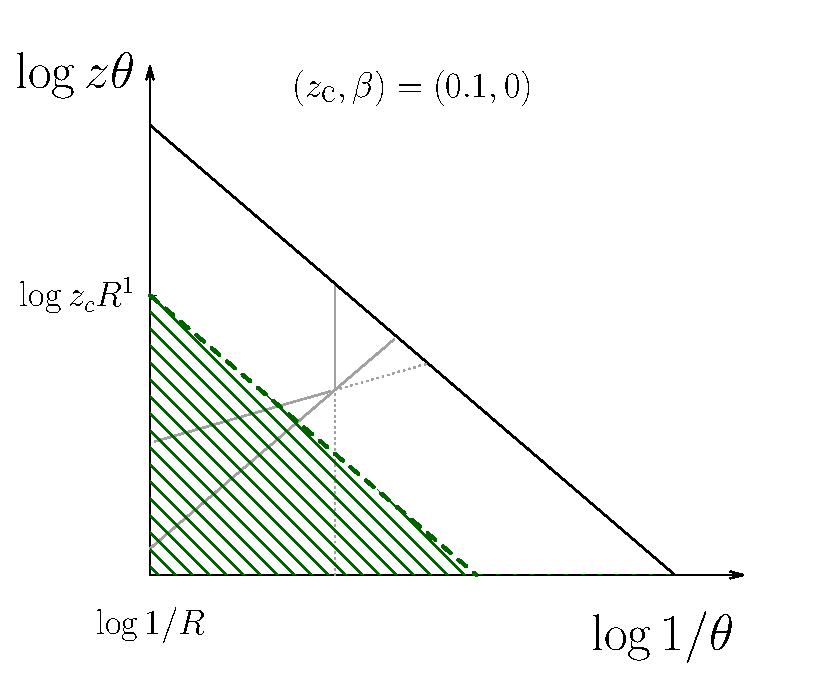
\includegraphics[width=0.33\textwidth]{figures/kinematics/plotVac_SD2_2}%
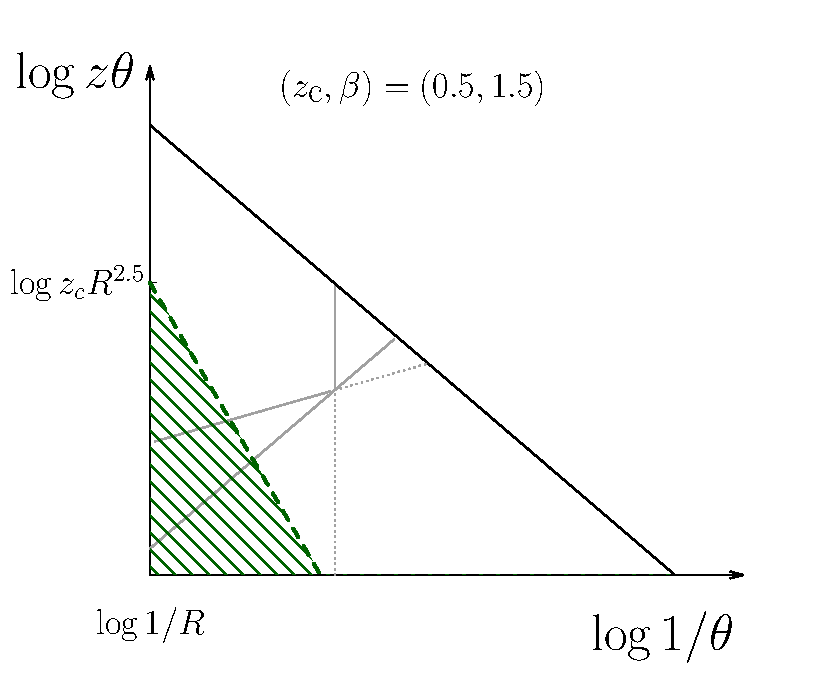
\includegraphics[width=0.33\textwidth]{figures/kinematics/plotVac_SD1_2}%
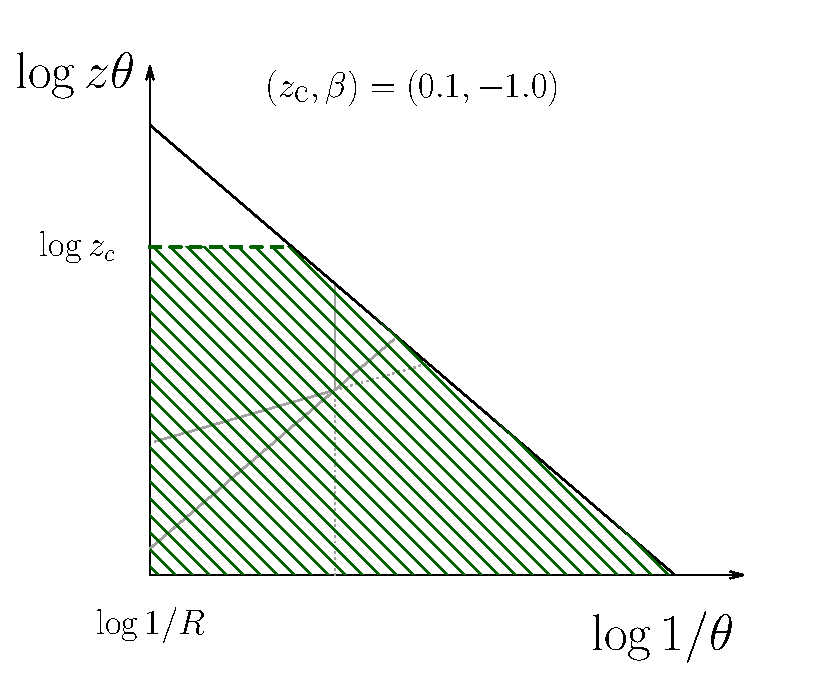
\includegraphics[width=0.33\textwidth]{figures/kinematics/plotVac_SD3_2}%
\caption{The three grooming settings studied in this report, see text for details. Shaded areas correspond to configuration that are groomed away.}
\label{fig:TheorySD}
\end{figure}
%%%%%%%%%%%%%%%%%%%%%%%%%%%%%%%%%%%%%
In this report, we compare the three grooming settings:
\begin{description}
\item[{\bf SD1:}] $z_{\text{cut}}=0.1$ and $\beta=0$: removes branches based only on the energy fraction;
\item[{\bf SD2:}]  $z_{\text{cut}}=0.5$ and $\beta=1.5$: has a stronger grooming at large angle;
\item[{\bf SD3:}]  $z_{\text{cut}}=0.1$ and $\beta=-1.0$: selects only hard radiation;
\end{description}
\autoref{fig:TheorySD} depicts how these settings remove parts of the phase space in the Lund plane. This will in turn affect the demands on statistics, especially for the SD3 setting. While the first setting is the more widely used in various studies of the SD procedure, the two latter are designed to suppress regions of phase space with a lot of medium activity, as identified in the diagrams in \autoref{fig:PS2}. One could, of course, devise other grooming strategies, or even combine various conditions, in order to ``carve'' out kinematical regimes of particular interest. We avoid such prescriptions here in order not to bias our jet sample excessively. On the other hand, it could be interesting to combine grooming strategies with specific reclustering algorithms, a point we briefly study in \autoref{sec:hadronization}.
%{\color{red} some more description needed}

%\begin{figure}[h]
%\centering
%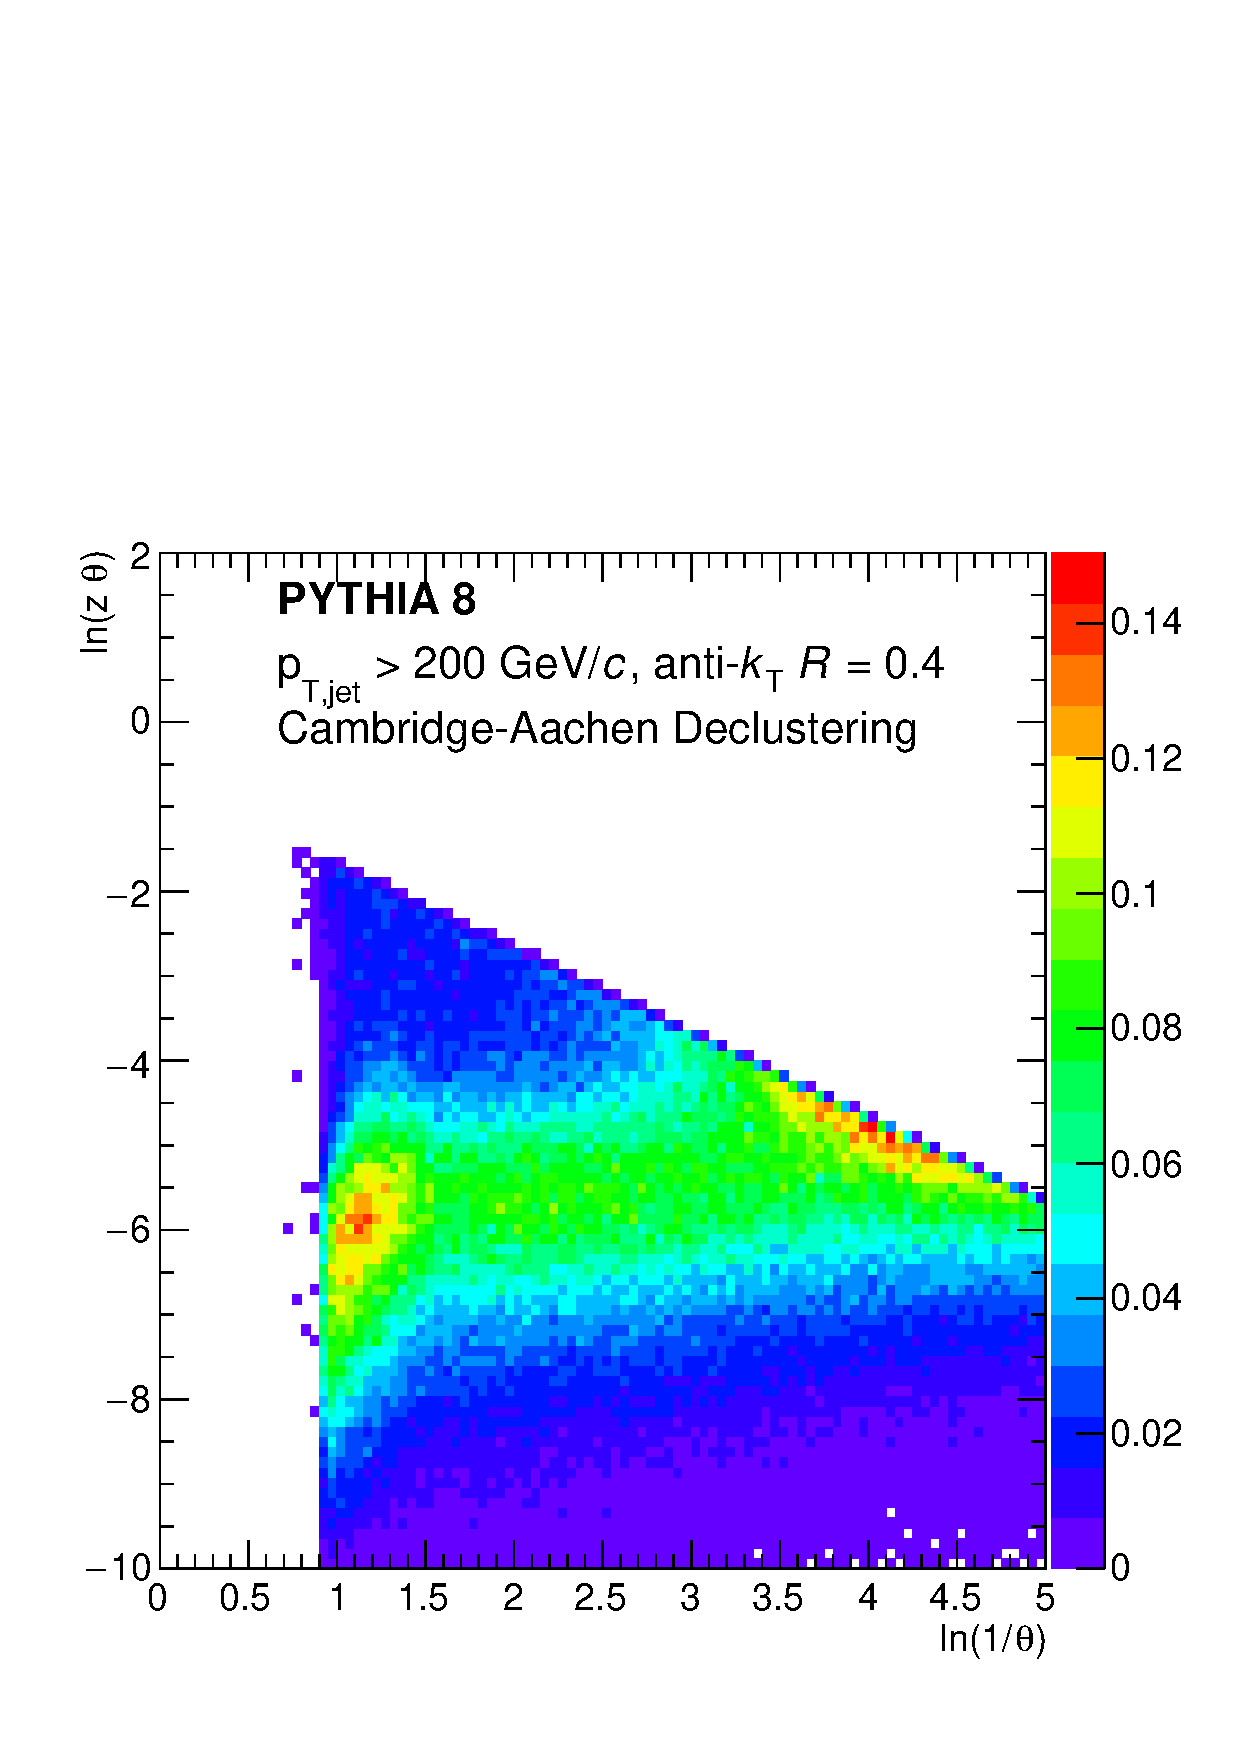
\includegraphics[width=0.33\textwidth]{figures/LundMC/Pythia_CA}
%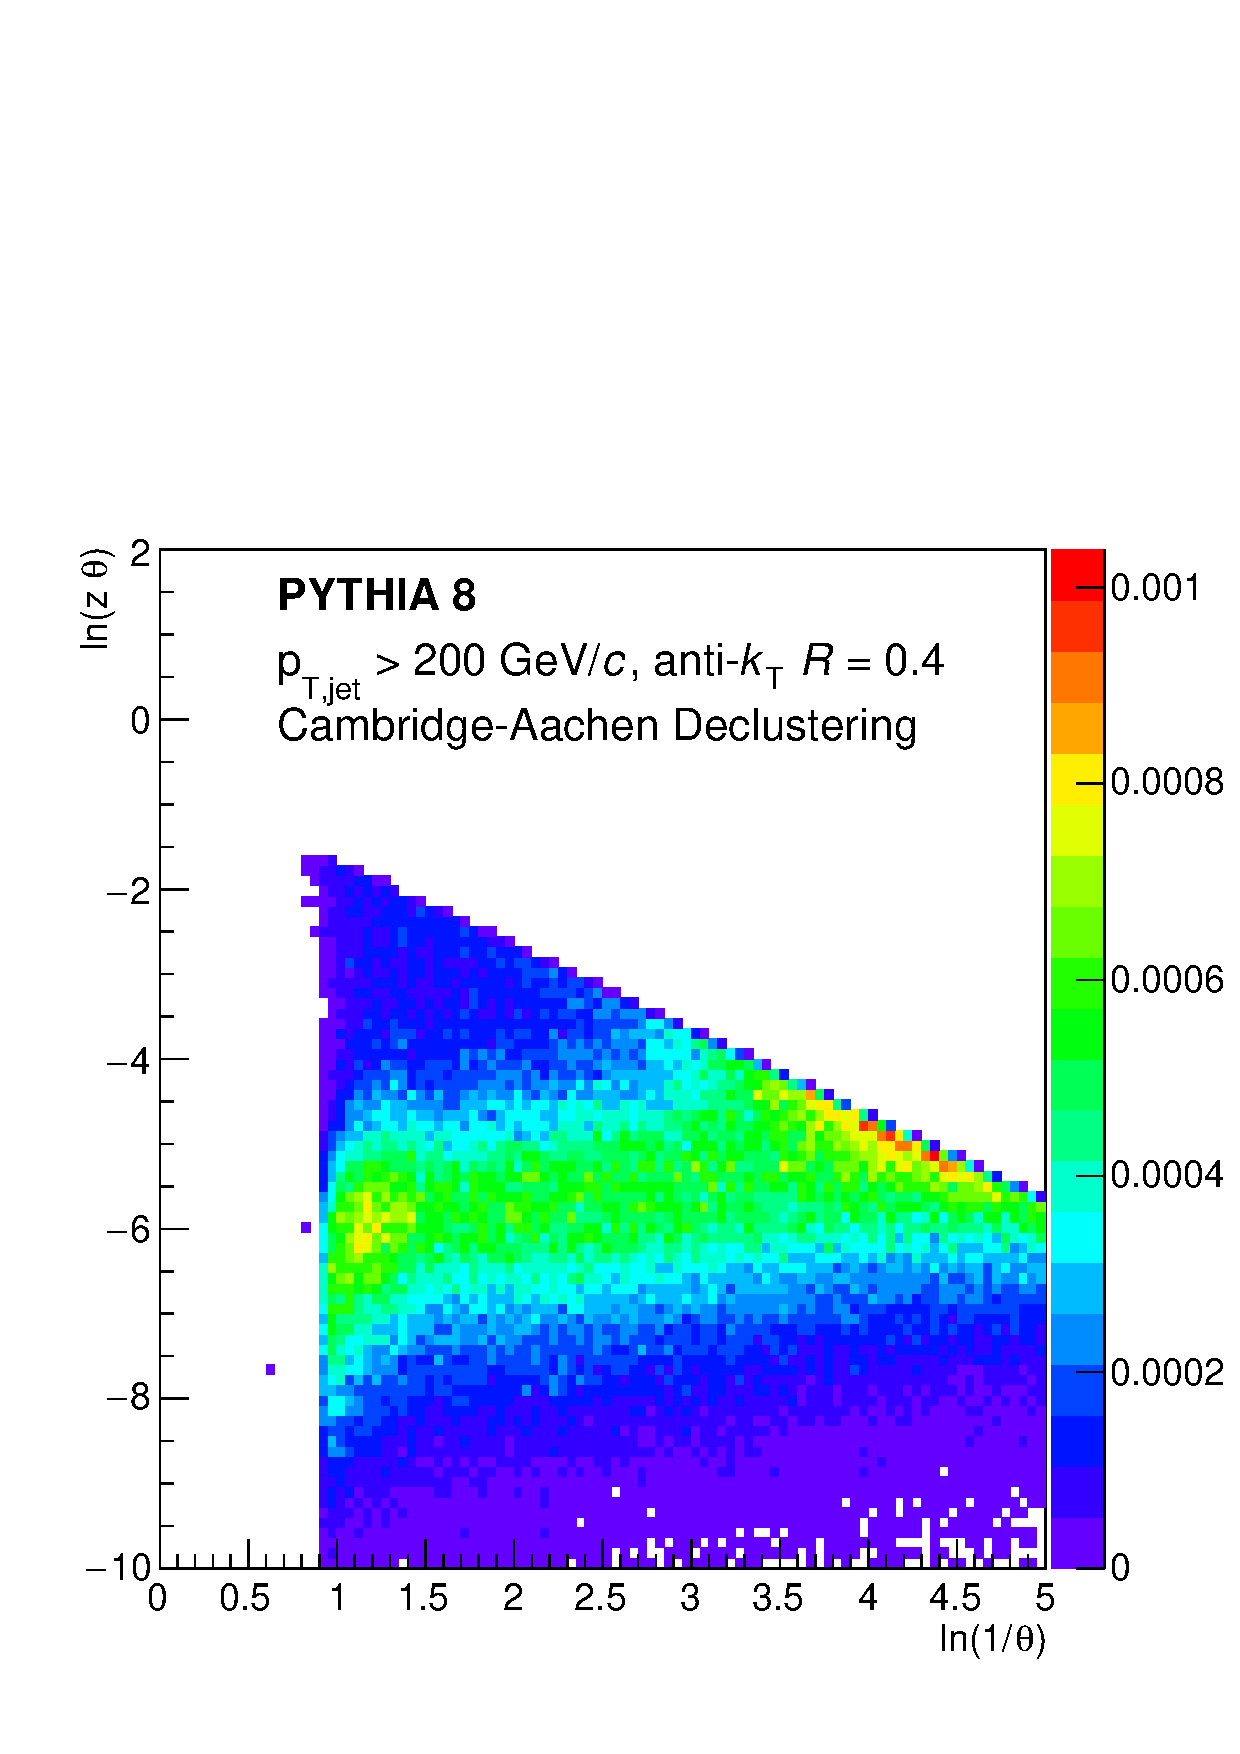
\includegraphics[width=0.33\textwidth]{figures/LundMC/Pythia_NoUE}
%\caption{Lund diagram reconstructed from jets generated by PYTHIA8 with (left) and without underlying event (right)}
%\label{fig:PS2Vac}
%\end{figure}
%introduce grooming; explaining clustering/declustering
%%%%%%%%%%%%%%%%%%%%%%%%%%%%%%%%%%%%%%%%%%%%%
%\subsection{Radiation phase space and sensitivity to jet quenching {\color{green} Leticia,Harry}}
%\label{sec:radiationPSJQ}
%%%%%%%%%%%%%%%%%%%%%%%%%%%%%%%%%%%%%%%%%%%%%
%\subsubsection{Medium-induced radiation}
%%%%%%%%%%%%%%%%%%%%%%%%%%%%%%%%%%%%%%
%\begin{figure}[h]
%\centering
%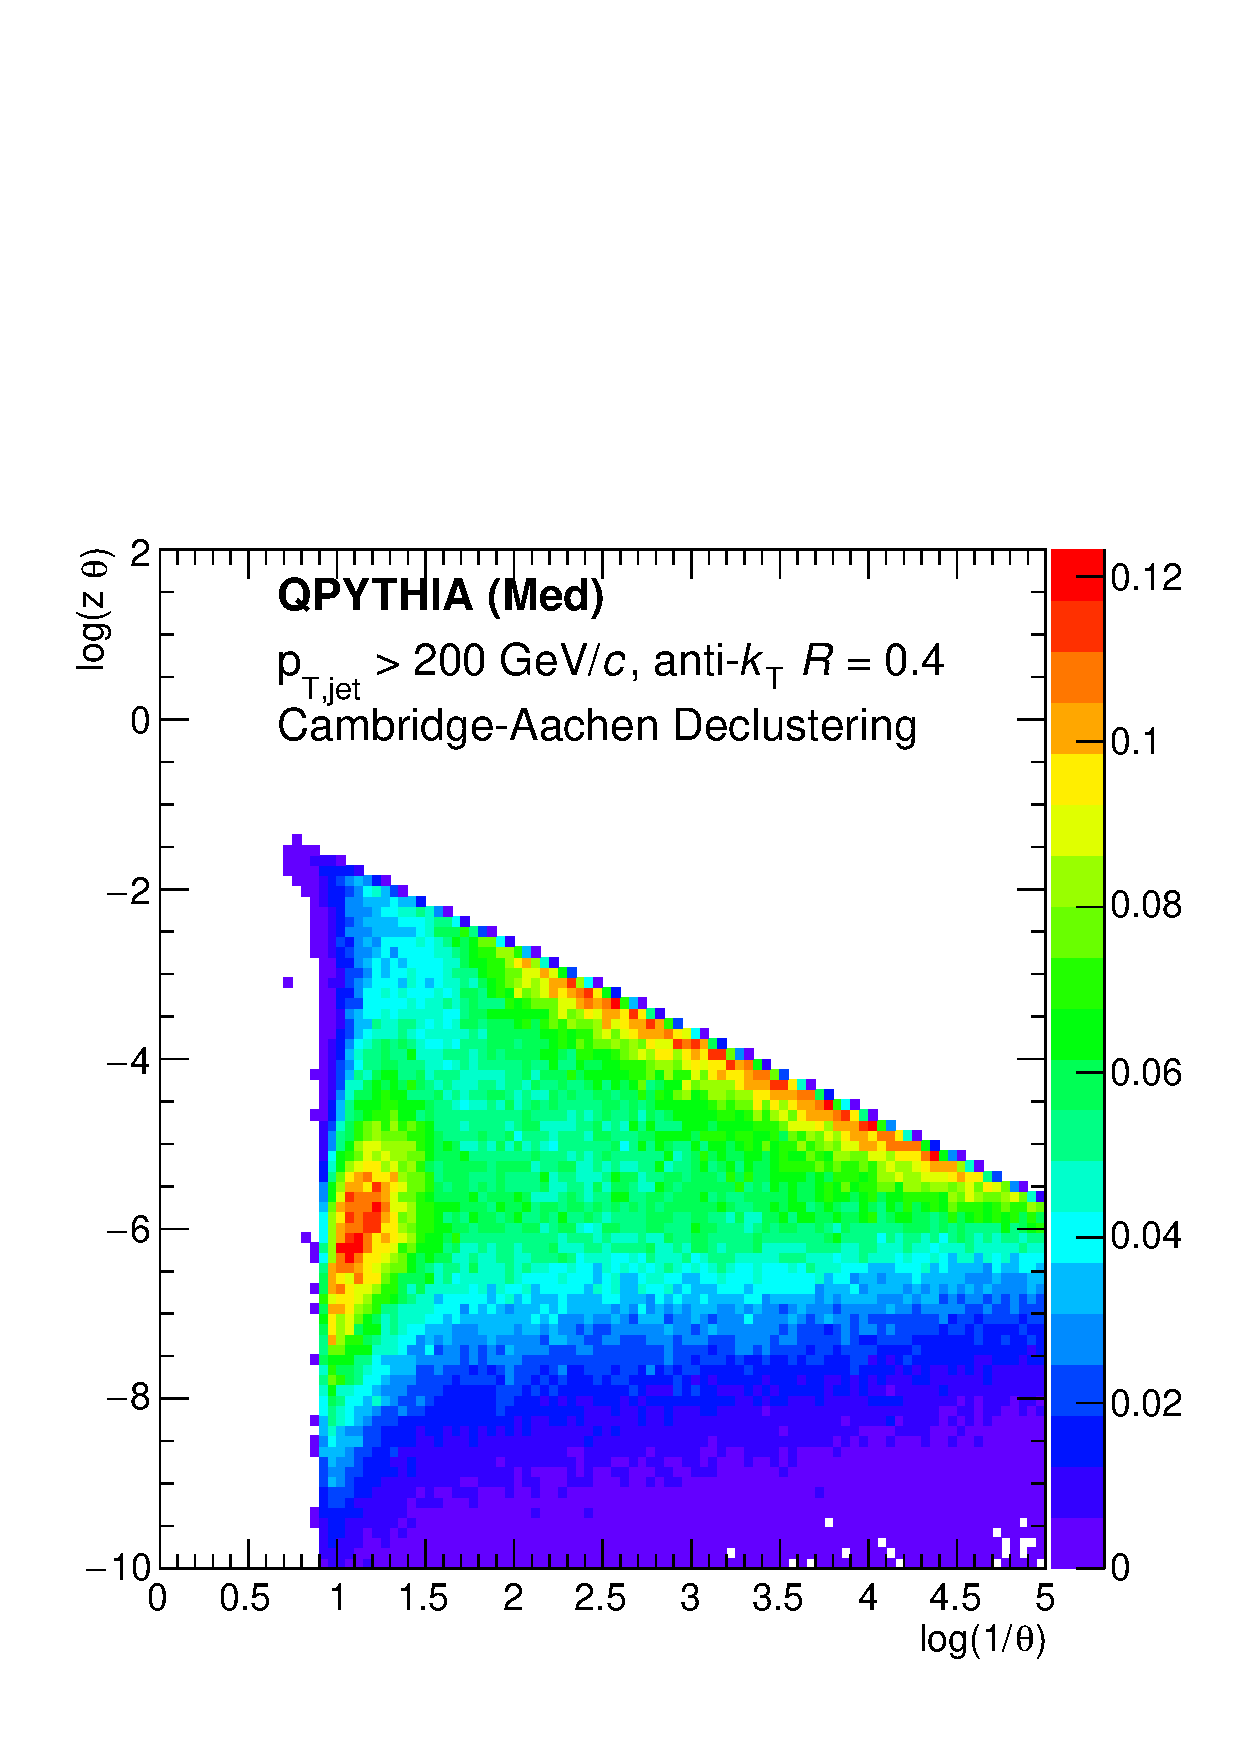
\includegraphics[width=0.3\textwidth]{figures/LundMC/QPythiaHyd200}
%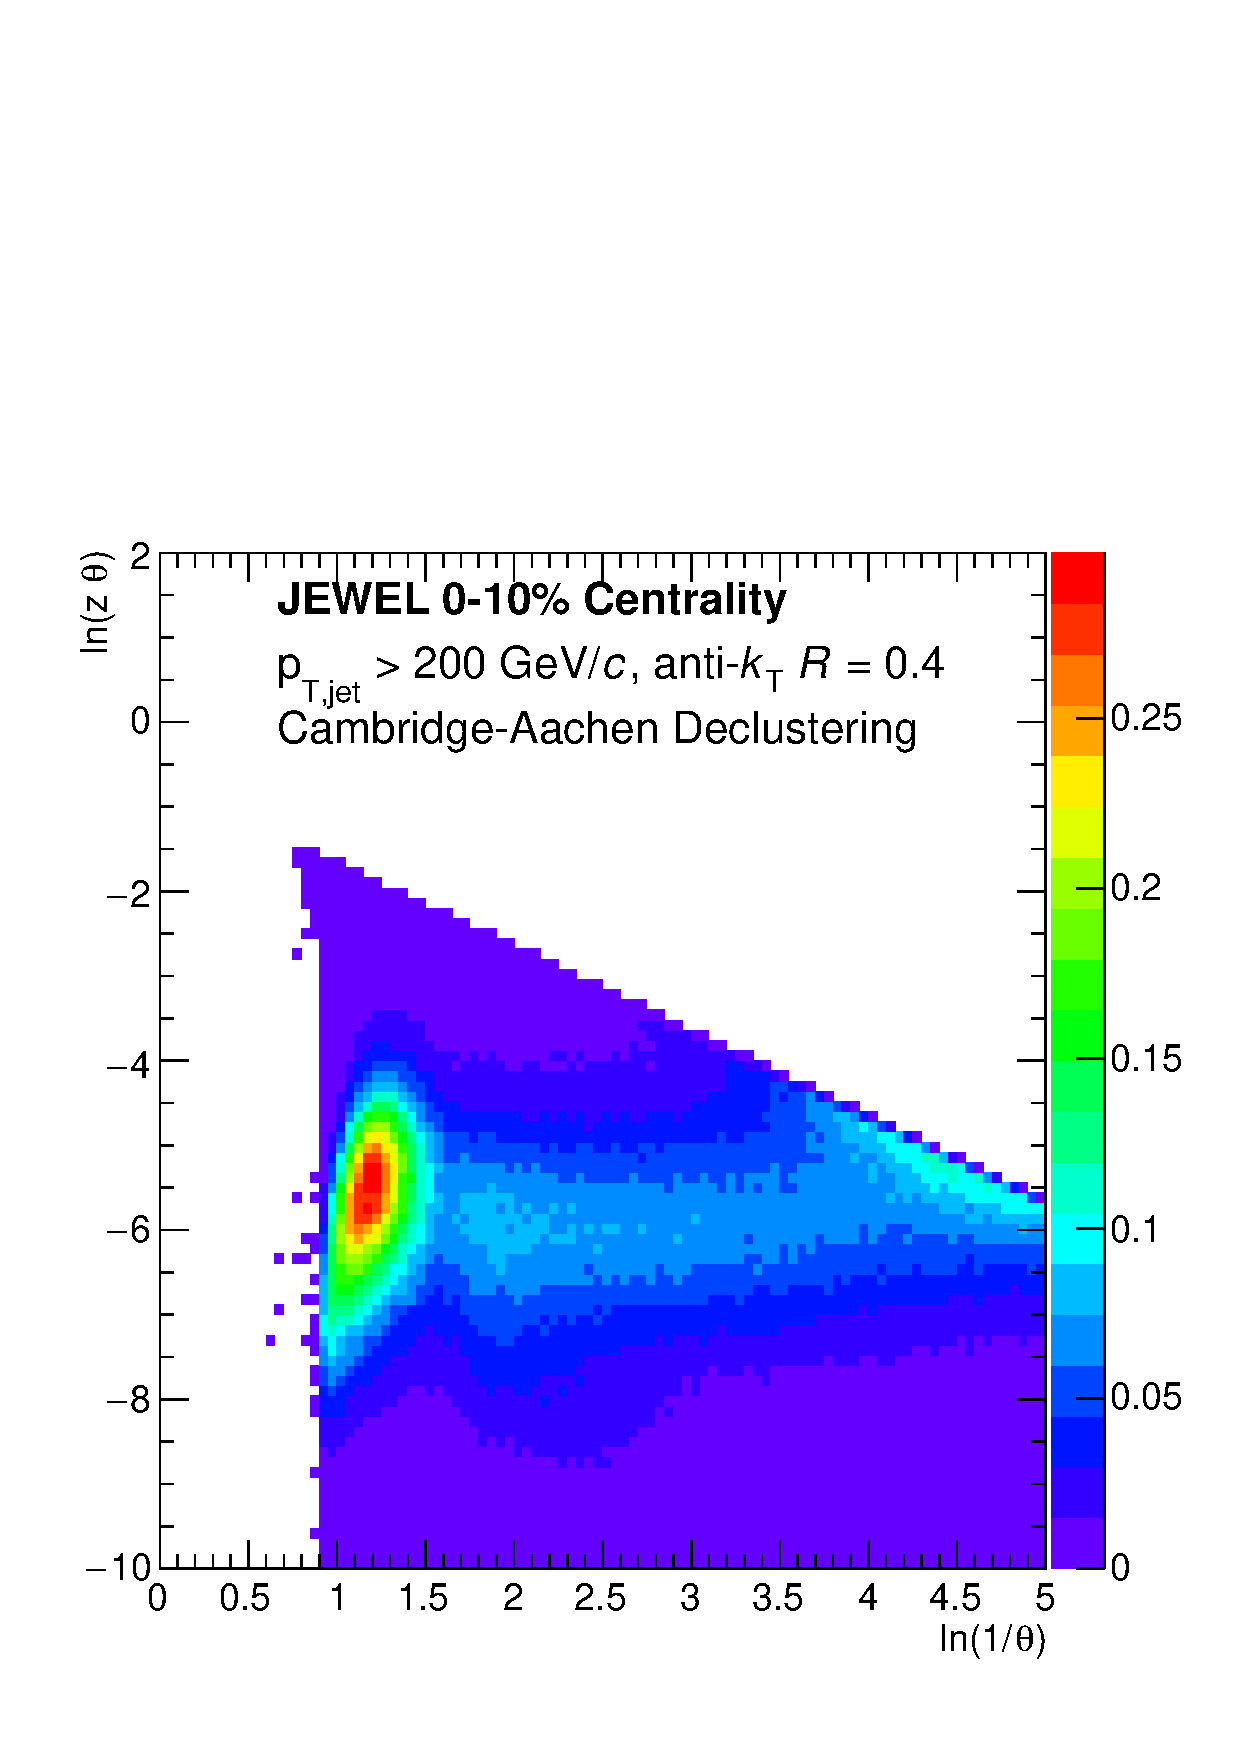
\includegraphics[width=0.3\textwidth]{figures/LundMC/JewelRecoilOff}
%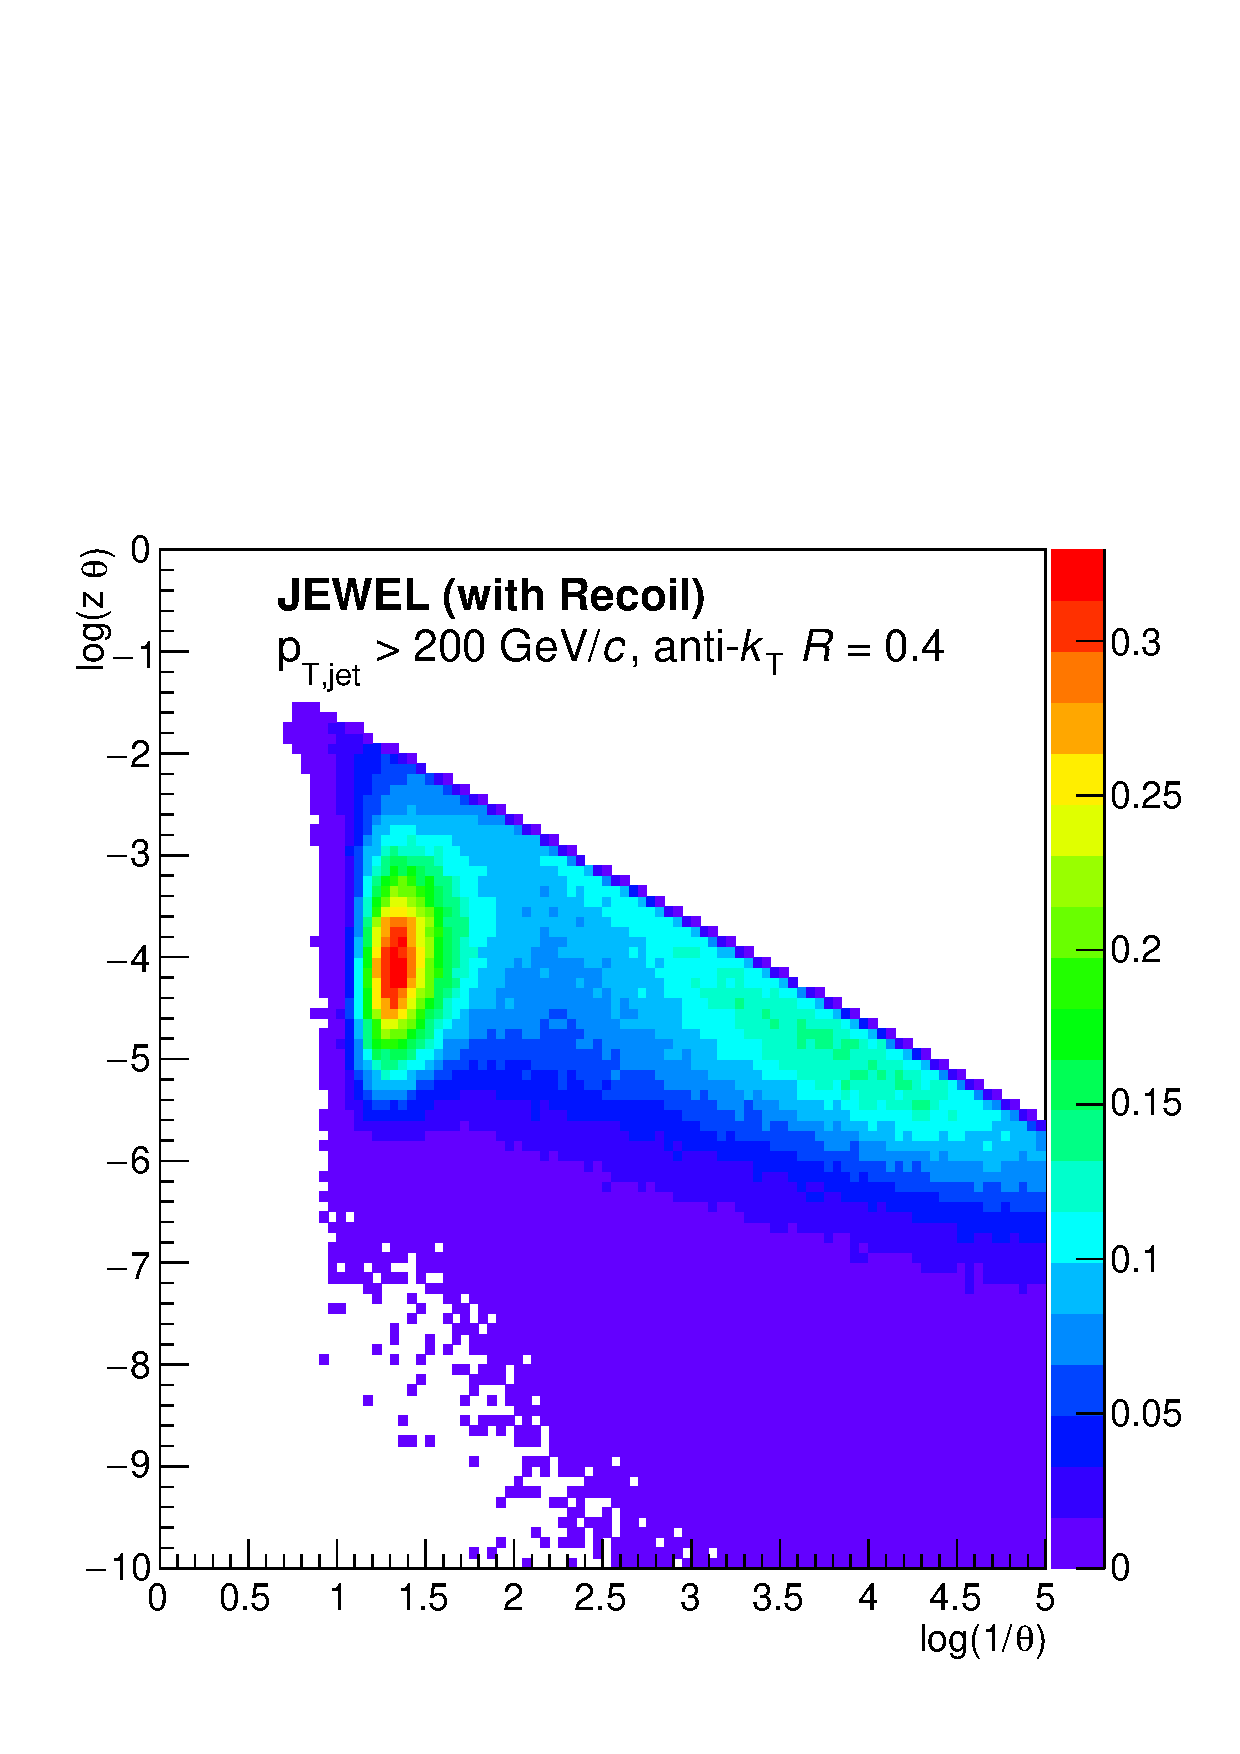
\includegraphics[width=0.3\textwidth]{figures/LundMC/JewelRecoilOn}
%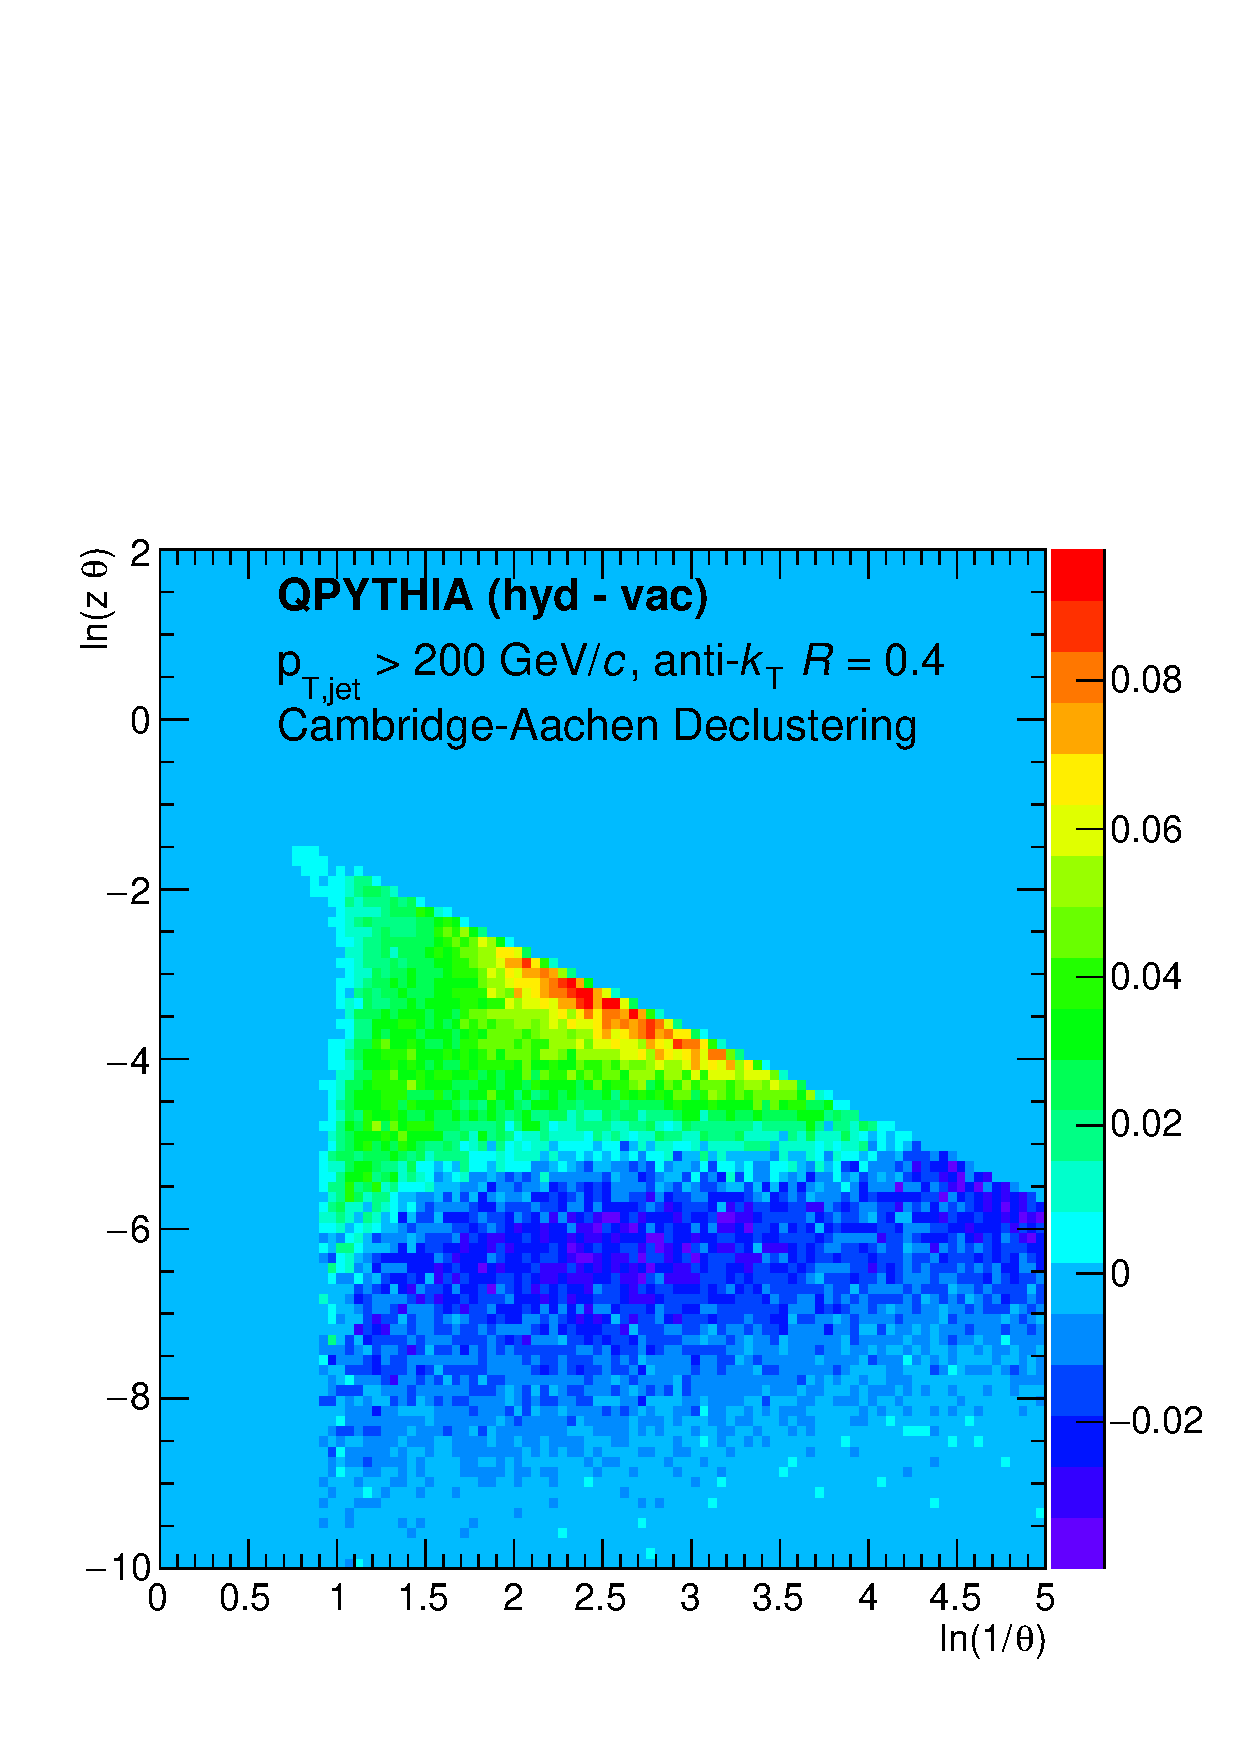
\includegraphics[width=0.3\textwidth]{figures/LundMC/QPythiaDiff200}
%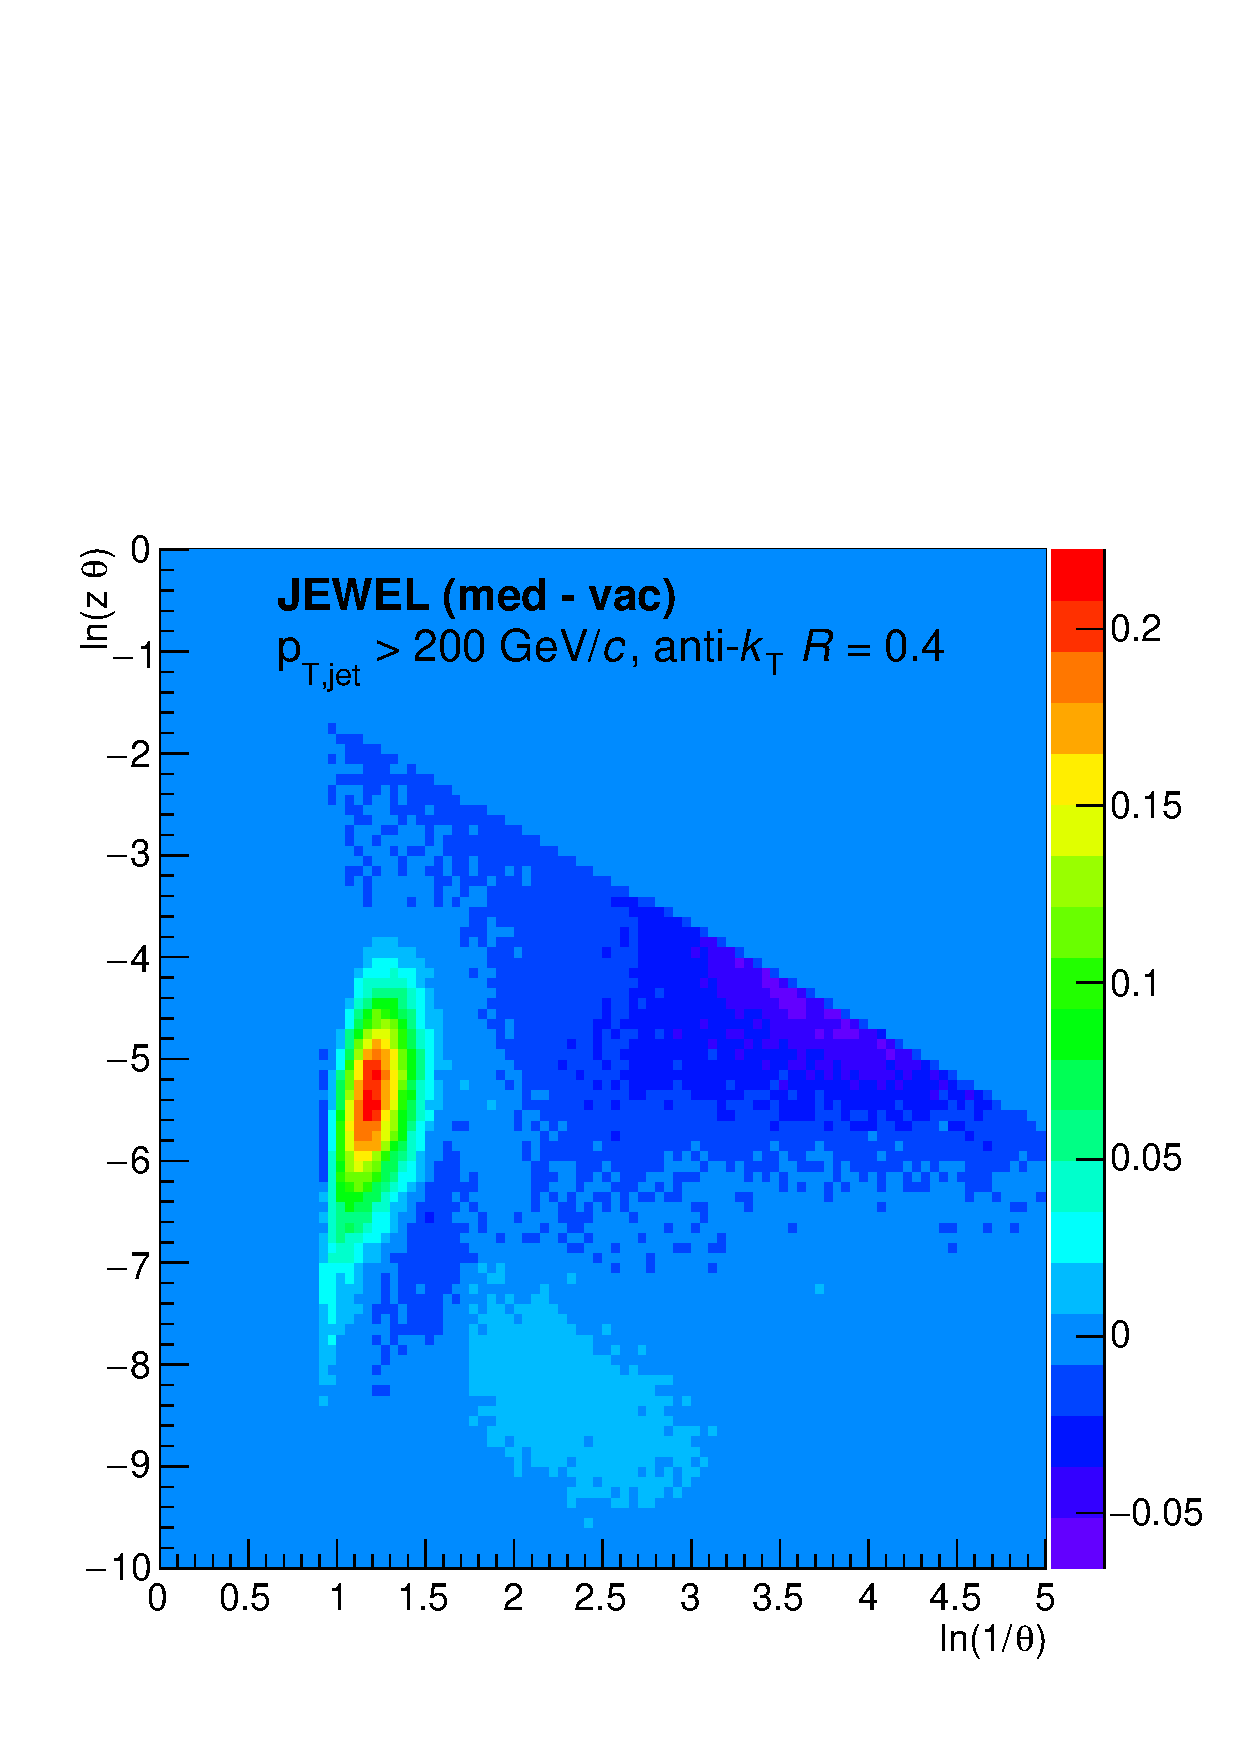
\includegraphics[width=0.3\textwidth]{figures/LundMC/JewelRecoilOffDiff}
%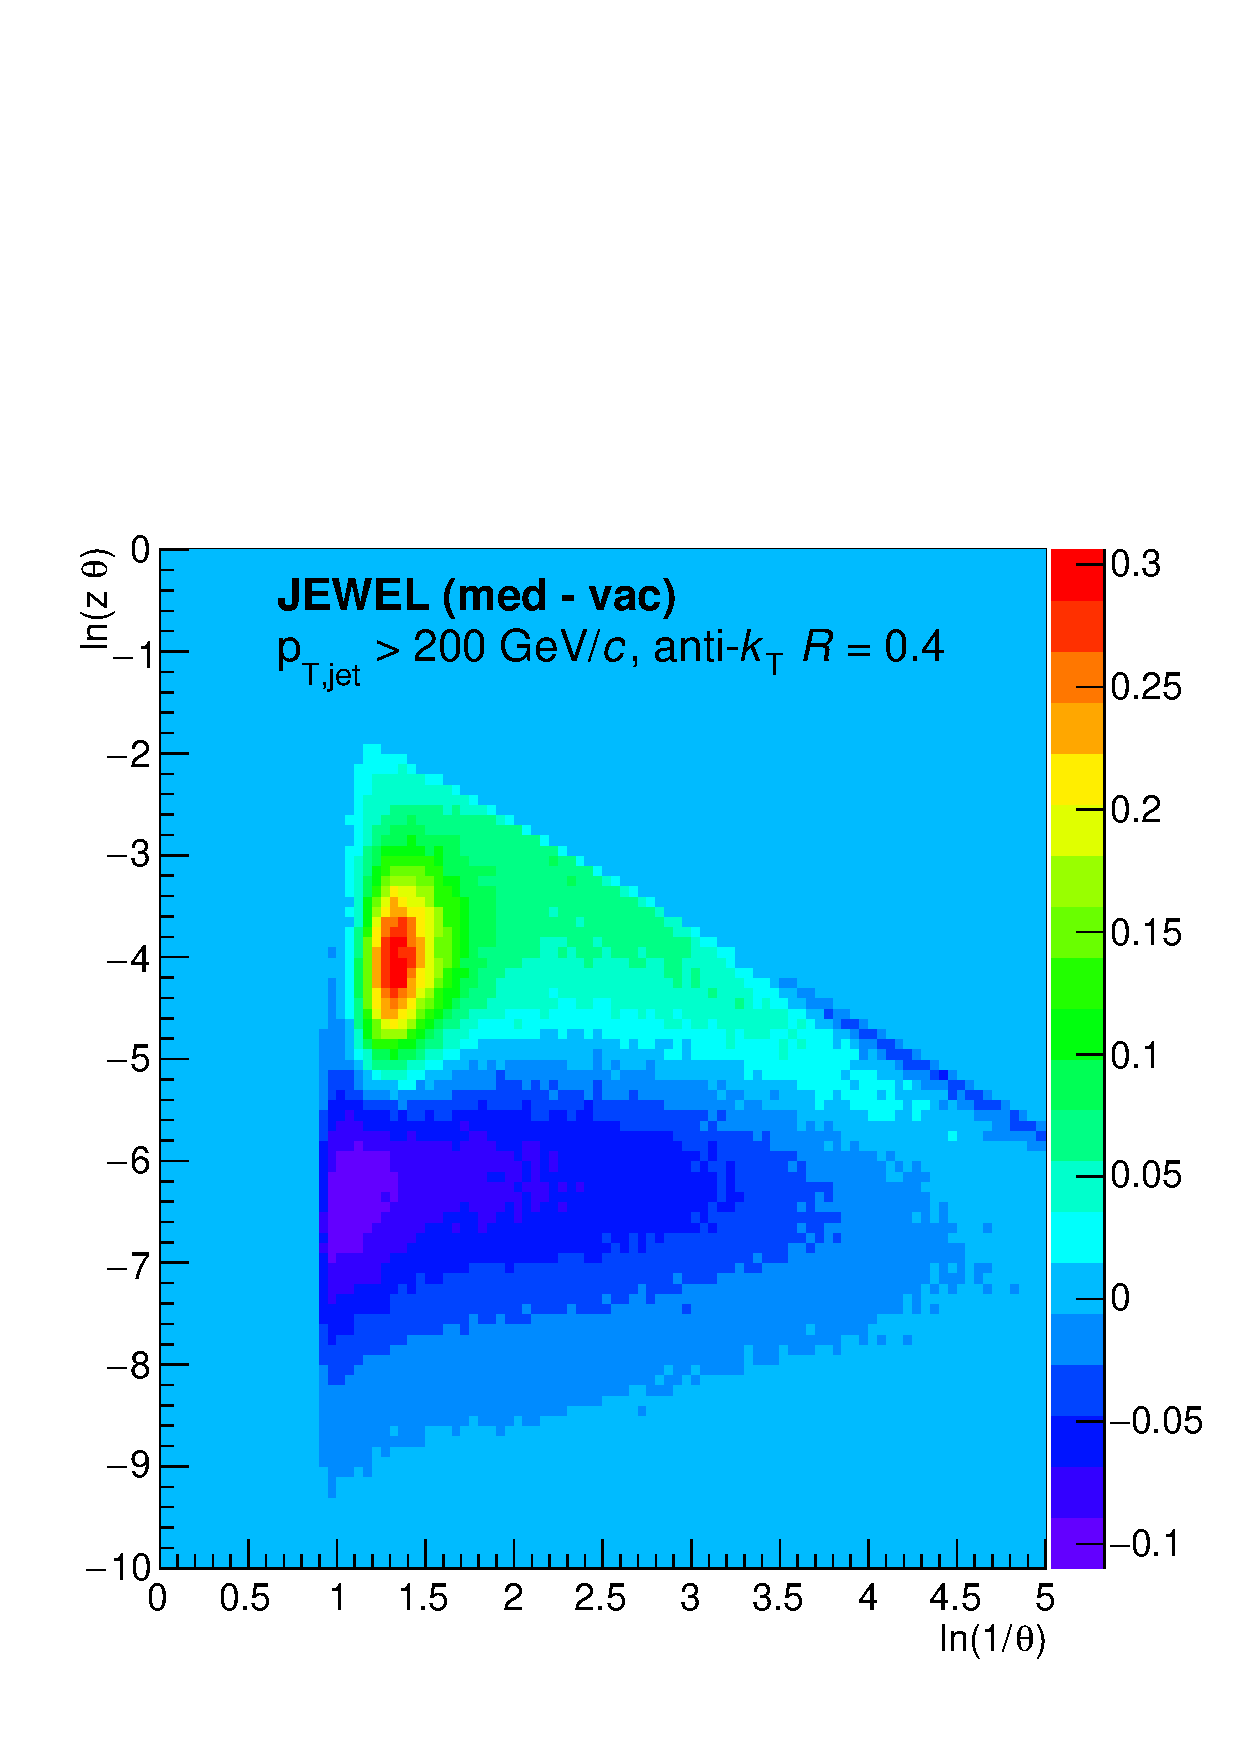
\includegraphics[width=0.3\textwidth]{figures/LundMC/JewelRecoilOnDiff}
%\caption{Lund diagram reconstructed from jets generated by QPYTHIA (left), JEWEL without recoils (middle) and JEWEL with recoils on.
%The lower panels correspond to the difference of the radiation pattern between with and without jet quenching.}
%\label{fig:PS2}
%\end{figure}
%%%%%%%%%%%%%%%%%%%%%%%%%%%%%%%%%%%%%%
%As a demonstration of the general ideas outlined above, we have filled the Lund diagram using PYTHIA 8, and two pQCD-based models for jet quenching, namely JEWEL (w/wo medium recoils) and QPYTHIA.  The variables $z\theta$ and $\theta$ have been reconstructed from subsequent branchings that were identified by reclustering the jet with a C/A algorithm.
%
%Fig.~\ref{fig:PS2Vac} shows the Lund diagram in vacuum and its characteristic horizontal bands due to the evolution of the coupling constant with the momentum scale are apparent. The excess of splittings at large angle seen in the left plot is caused by the PYTHIA underlying event, which is switched off in the right plot. 
%
%Fig.~\ref{fig:PS2}, upper plots, correspond to QPYTHIA, JEWEL w/o recoils and JEWEL w/ recoils respectively. The lower plots show the differences to the corresponding vacuum Lund diagrams.
%
%QPYTHIA exhibits an modest excess of large $k_{T}$ quanta relative to vacuum. In the model, the number of splittings is increased relative to vacuum leading to a significant intra-jet momentum broadening. 
%
%JEWEL generates additional medium-induced branchings that are not present in the vacuum reference. These are also allowed to branch further in the medium. In the difference plot we can clearly identify a modest excess of large-angle, semi-hard quanta in JEWEL. Interestingly, jet profiles calculated with JEWEL do not show an enhancement of momentum at large angles relative to vacuum \cite{KunnawalkamElayavalli:2017hxo}. A possible reason is that in the case of the jet profiles the angle is always measured relative to the jet axis while in our declustering approach the angles are always measured relative to the hardest parent or subjet, in which case the angular distribution can be broader. 
%Such excess becomes harder when the medium recoils are included. The nature and role of the recoils will be explained in the next subsection. 
%
%It is worth noting that the medium-induced signal populates different regions of phase space in the two jet quenching models. The choice of the grooming parameters in Eq. \ref{eq:groompar} is critical to enhance the sensitivity to the signal, as it will be discussed in the next section. 
%
%
%\subsubsection{Medium response}
%
%Jet quenching is expected to be accompanied by recoil effects. The jet induced medium response constitutes a correlated background that can contribute to the modifications of the measured jet substructure. Recoil effects are expected to contribute in the soft-large angle sector of the phase space, similarly to the uncorrelated underlying event, described in the next section. 
%
%JEWEL can be ran with and without recoiling partons entering the hadronisation. 
%The difference between the Lund diagrams for the two options is shown in Fig.~\ref{fig:PS2} lower right plot. 
%
%The impact of the recoils as modeled by JEWEL has being documented \cite{Milhano:2017nzm}\cite{KunnawalkamElayavalli:2017hxo}. Its contribution is needed to describe most of the jet shapes measured so far at the LHC. In particular, if the medium response can smear the subleading subjet momentum above the given grooming cut, the subjet momentum balance or $z_{g}$ can become more asymmetric relative to vacuum.   
%
%As a correlated background, the medium response cannot be experimentally subtracted
%to isolate purely radiative modifications to the jet shower. However, correlation of jet substructure observables might help to suppress it \cite{Milhano:2017nzm}. 
%\begin{figure}[th]
%\centering
%\includegraphics[width=0.33\textwidth]{figures/LundMC/JewelRecoilDiff.pdf}%
%\caption{Difference of the lund plots for JEWEL with recoils on and without}
%\label{fig:RecoilJewel}
%\end{figure}

%\clearpage
%\newpage
%%%%%%%%%%%%%%%%%%%%%%%%%%%%%%%%%%%%%
\subsection{Groomed substructure observables and sensitivity to jet quenching}
\label{sec:groomedobservables}
%%%%%%%%%%%%%%%%%%%%%%%%%%%%%%%%%%%%%

After identifying the first splitting that satisfies Eq.~(\ref{eq:groompar}), we have access to the full kinematics of that branching process. The groomed jet energy ($\pT = E$) is now defined as $p_{{\rm \tiny T} g} \equiv p_{\mathrm{T},1}+p_{\mathrm{T},2}$, where the subscripts now refer to the identified subjets. We can then define the groomed momentum fraction, $z_g = \min \left(p_{{\rm \tiny T},1},p_{{\rm \tiny T},2}\right)/p_{{\rm \tiny T}g}$ and the angle $\Delta R_{12}$ between the subjets. In our numerical studies, we will focus on these two quantities but also introduce the groomed mass to energy ratio $M_g/\pT$, where $M_g$ is defined as in Eq.~(\ref{eq:DipoleMass}) with all relevant quantities being groomed. These observables shed light on how the branchings occur in course of the parton shower and are sensitive to medium effects as long as the branching originates from inside the medium, roughly corresponding to $ t_{{\rm f}g}\equiv 2 p_{{\rm \tiny T}g}/M_g^2 < L$, see discussion above. For the chosen medium parameters, the samples analyzed with settings SD1 and SD2 will contain an admixture of in-medium and out-of-medium splittings, see \autoref{fig:TheorySD}, while SD3 picks exclusively out hard splittings originating from inside the medium. 

As in the previous section, the jet quenching Monte Carlo event generators we use in our study are QPYTHIA and JEWEL (with recoil effects turned on and off) and are shown in \autoref{fig:SDGenZG}, \ref{fig:SDGenDR12} and \ref{fig:SDGenMg}. Jets were reconstructed using anti-$k_{\rm \tiny T}=0.4$ and for $\pT > 130$ GeV/c. 
The results in this section are obtained at generator level, without embedding. In particular, we have not introduced any detector resolution effects, such as a minimal angular cut-off $\Delta R_{\rm min}$.
Note, that the distributions are normalized by the total number of anti-$k_{\text{T}}$ (ungroomed) jets. The distributions are therefore not self-normalized and contain information how grooming affects the overall suppression of the jet yield. 

%%%%%%%%%%%%%%%%%%%%%%%%%%%%%%%%%%%%%
\begin{figure}[t]
\centering
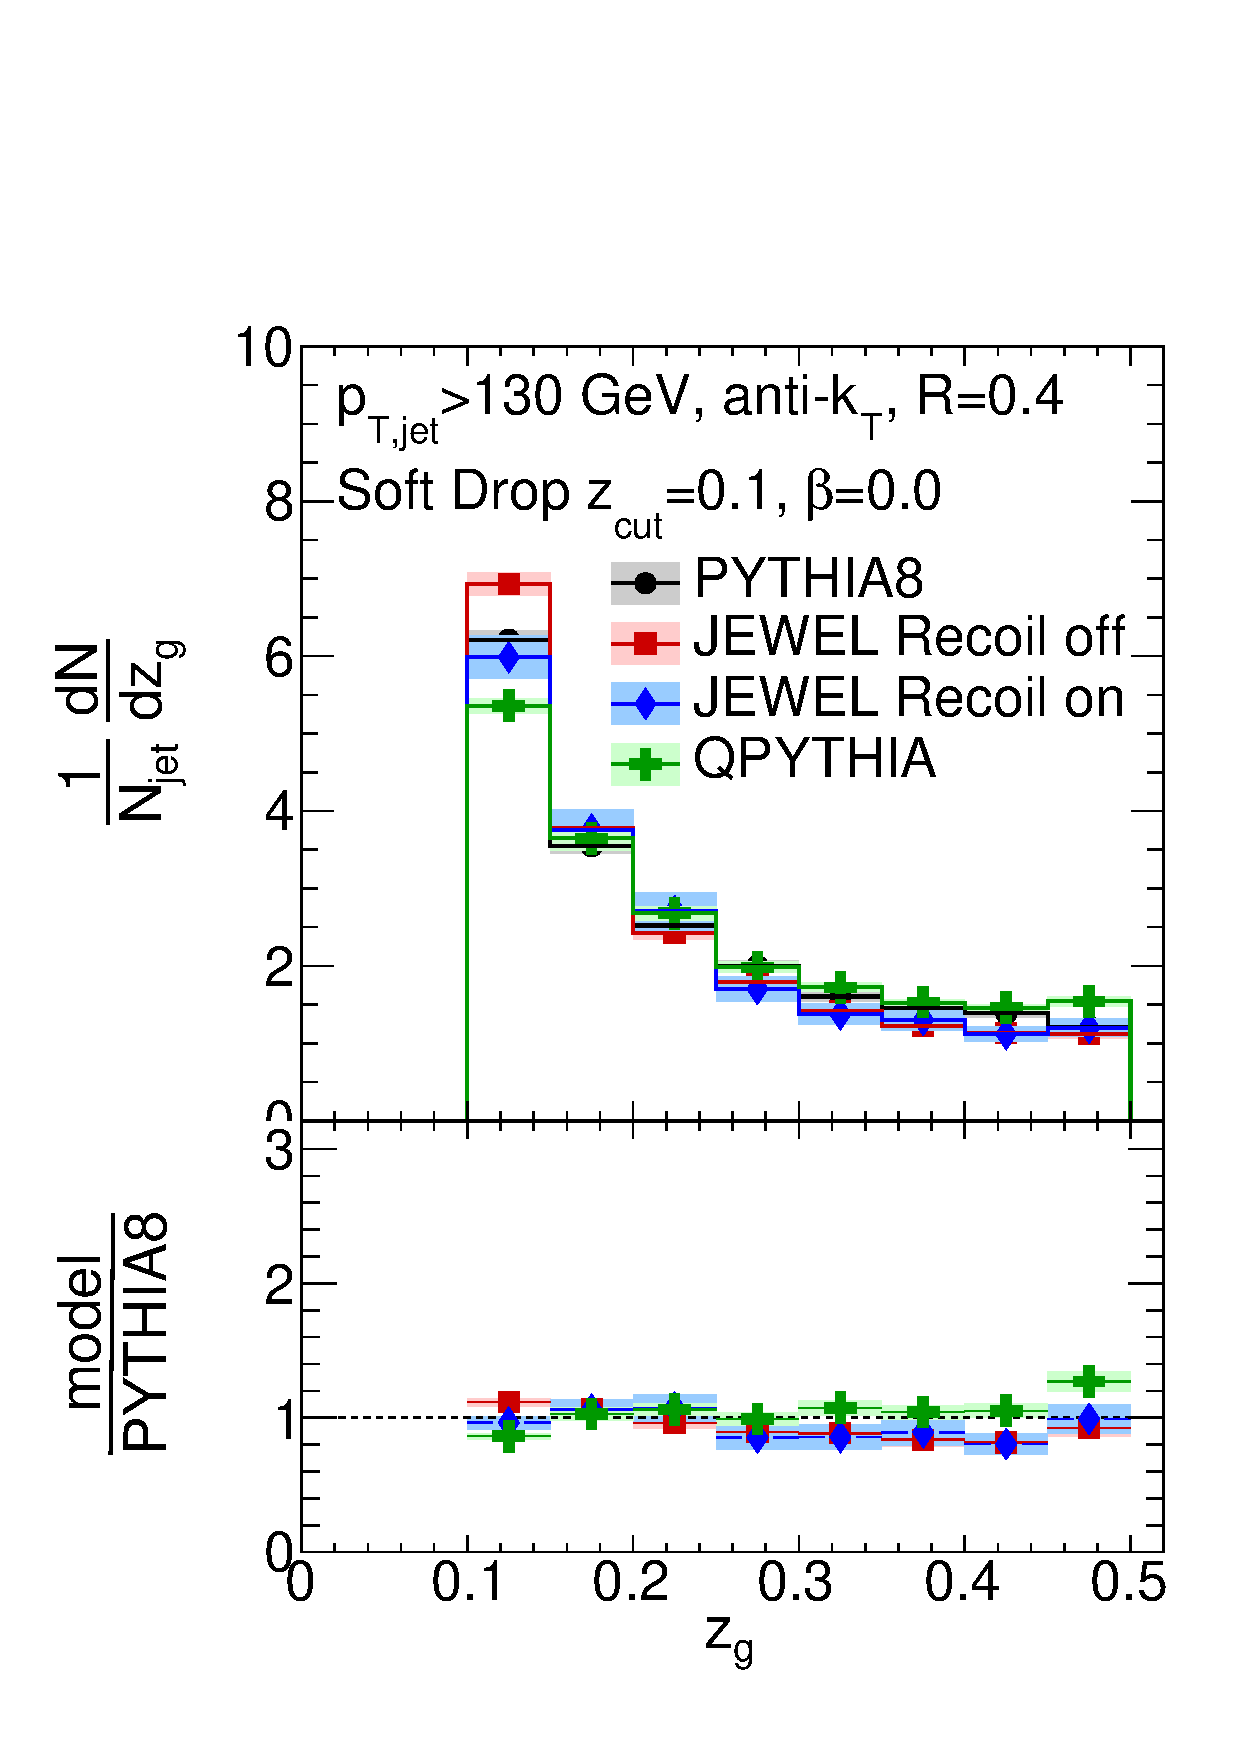
\includegraphics[width=0.33\textwidth]{figures/SDGen/ZgCompModelsBeta00Z01.pdf}%
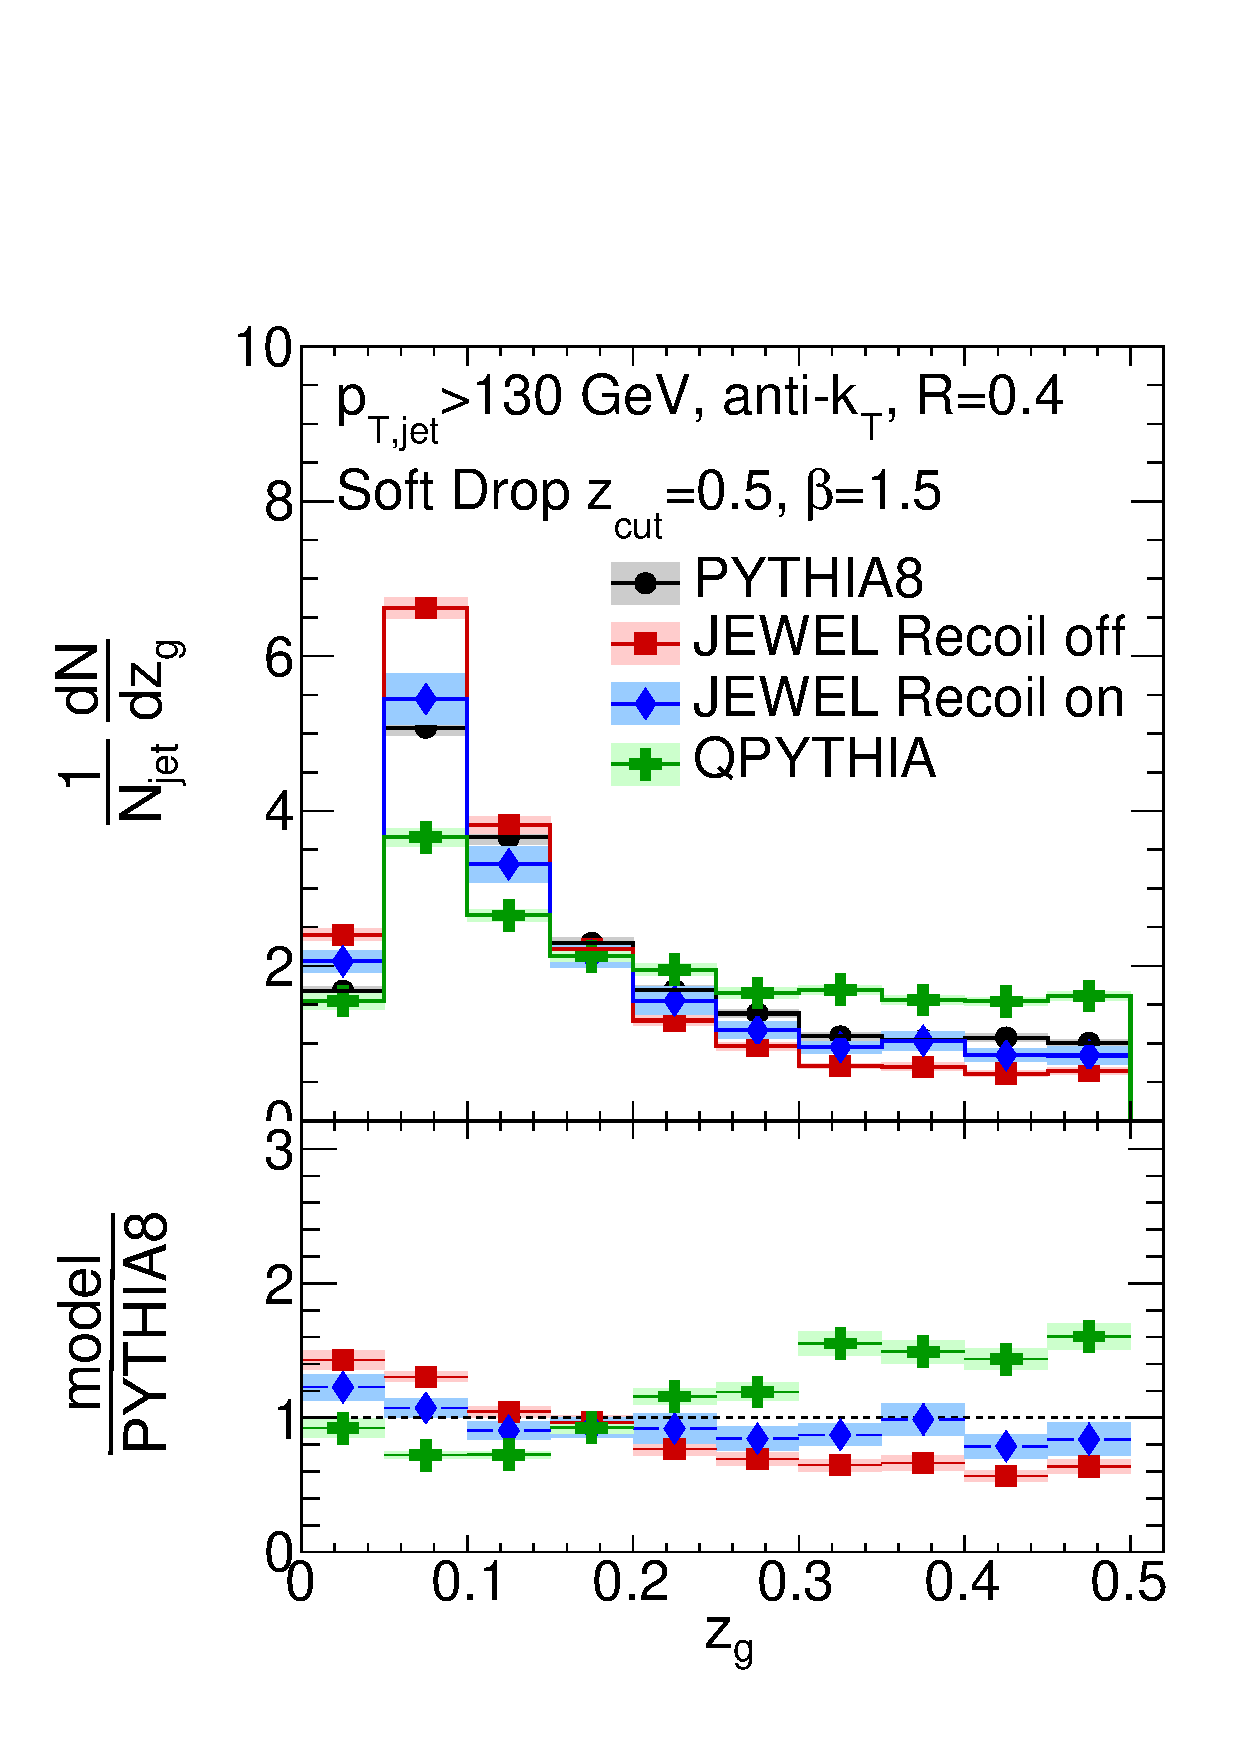
\includegraphics[width=0.33\textwidth]{figures/SDGen/ZgCompModelsBeta15Z05.pdf}%
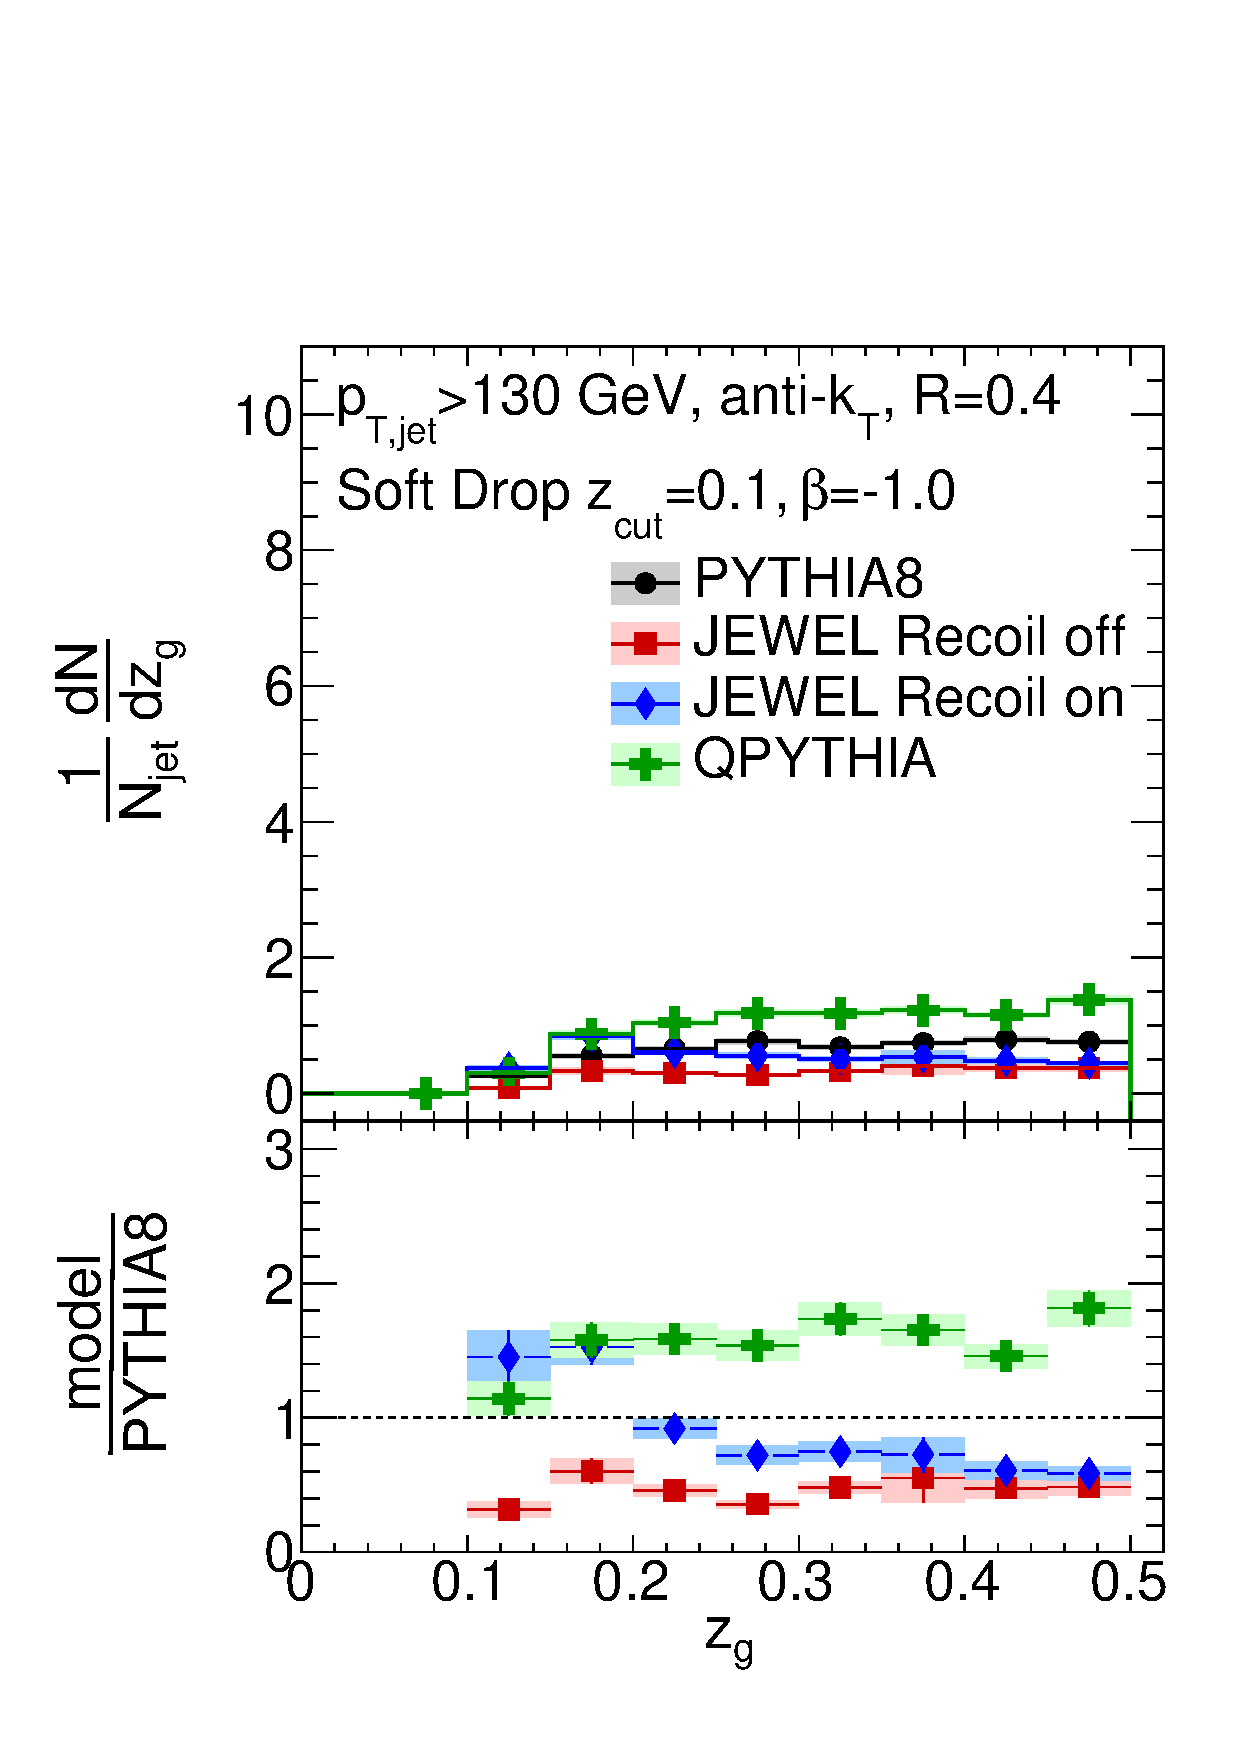
\includegraphics[width=0.33\textwidth]{figures/SDGen/ZgCompModelsBetam1Z01.pdf}%
\caption{Groomed shared momentum fraction, $z_{\mathrm{g}}$, for three different grooming settings in simulations with and without jet quenching. The uppers panels show the $z_{\mathrm{g}}$ distribution normalized by the total number of ungroomed jets while the lower panels show the ratio of JEWEL and QPYTHIA with respect to PYTHIA8.}
\label{fig:SDGenZG}
\end{figure}
%%%%%%%%%%%%%%%%%%%%%%%%%%%%%%%%%%%%%
Figure~\ref{fig:SDGenZG} shows the momentum fraction $z_g$ distribution for different event generators. The vacuum baseline is represented by the PYTHIA8 data points and compared to results from the QPYTHIA and JEWEL jet quenching event generators.
In this figure, the perhaps most striking feature is the generally opposite trend of the two models. This can also be traced back to the discussion around \autoref{fig:PS2}. The modified parton shower in QPYTHIA makes the jets broader with respect to jets in vacuum and therefore many more jets survive the grooming. JEWEL however collimates the jets and therefore less jets are surviving the grooming with this setting.

We also note, that while for $\beta \geq 0$, see \autoref{fig:SDGenZG} (left and center), the number of jets for the different generators remains roughly constant while for the negative grooming setting $\beta < 0$, \autoref{fig:SDGenZG} (right), a large deviation from unity can be observed. Interestingly, QPYTHIA subjets are strongly enhanced in this regime while JEWEL ``Recoils off'' subjets are strongly suppressed, both by a factor $\sim1.5-2$. Note also that the magnitude of effects are the biggest for the most aggressive setting that naively corresponds to early in-medium splittings.

Comparing the JEWEL results with and without recoil demonstrates that, for the chosen analysis settings, this observable is not very sensitive to recoil effects except for the small-$z_g$ region.
%The tightest setting $\beta < 0$ is notably very resilient.
In order to compare to the data presented in \cite{Sirunyan:2017bsd} for the $\beta=0$ setting, see also \cite{Milhano:2017nzm} for a study using JEWEL, where a significant deviation from vacuum baseline was observed, we again point out that no minimal angular cut-off was employed in our studies. Such a cut-off suppresses collinear vacuum radiation and, hence, amplifies the effects related to the medium.

%%%%%%%%%%%%%%%%%%%%%%%%%%%%%%%%%%%%%
\begin{figure}[th!]
\centering
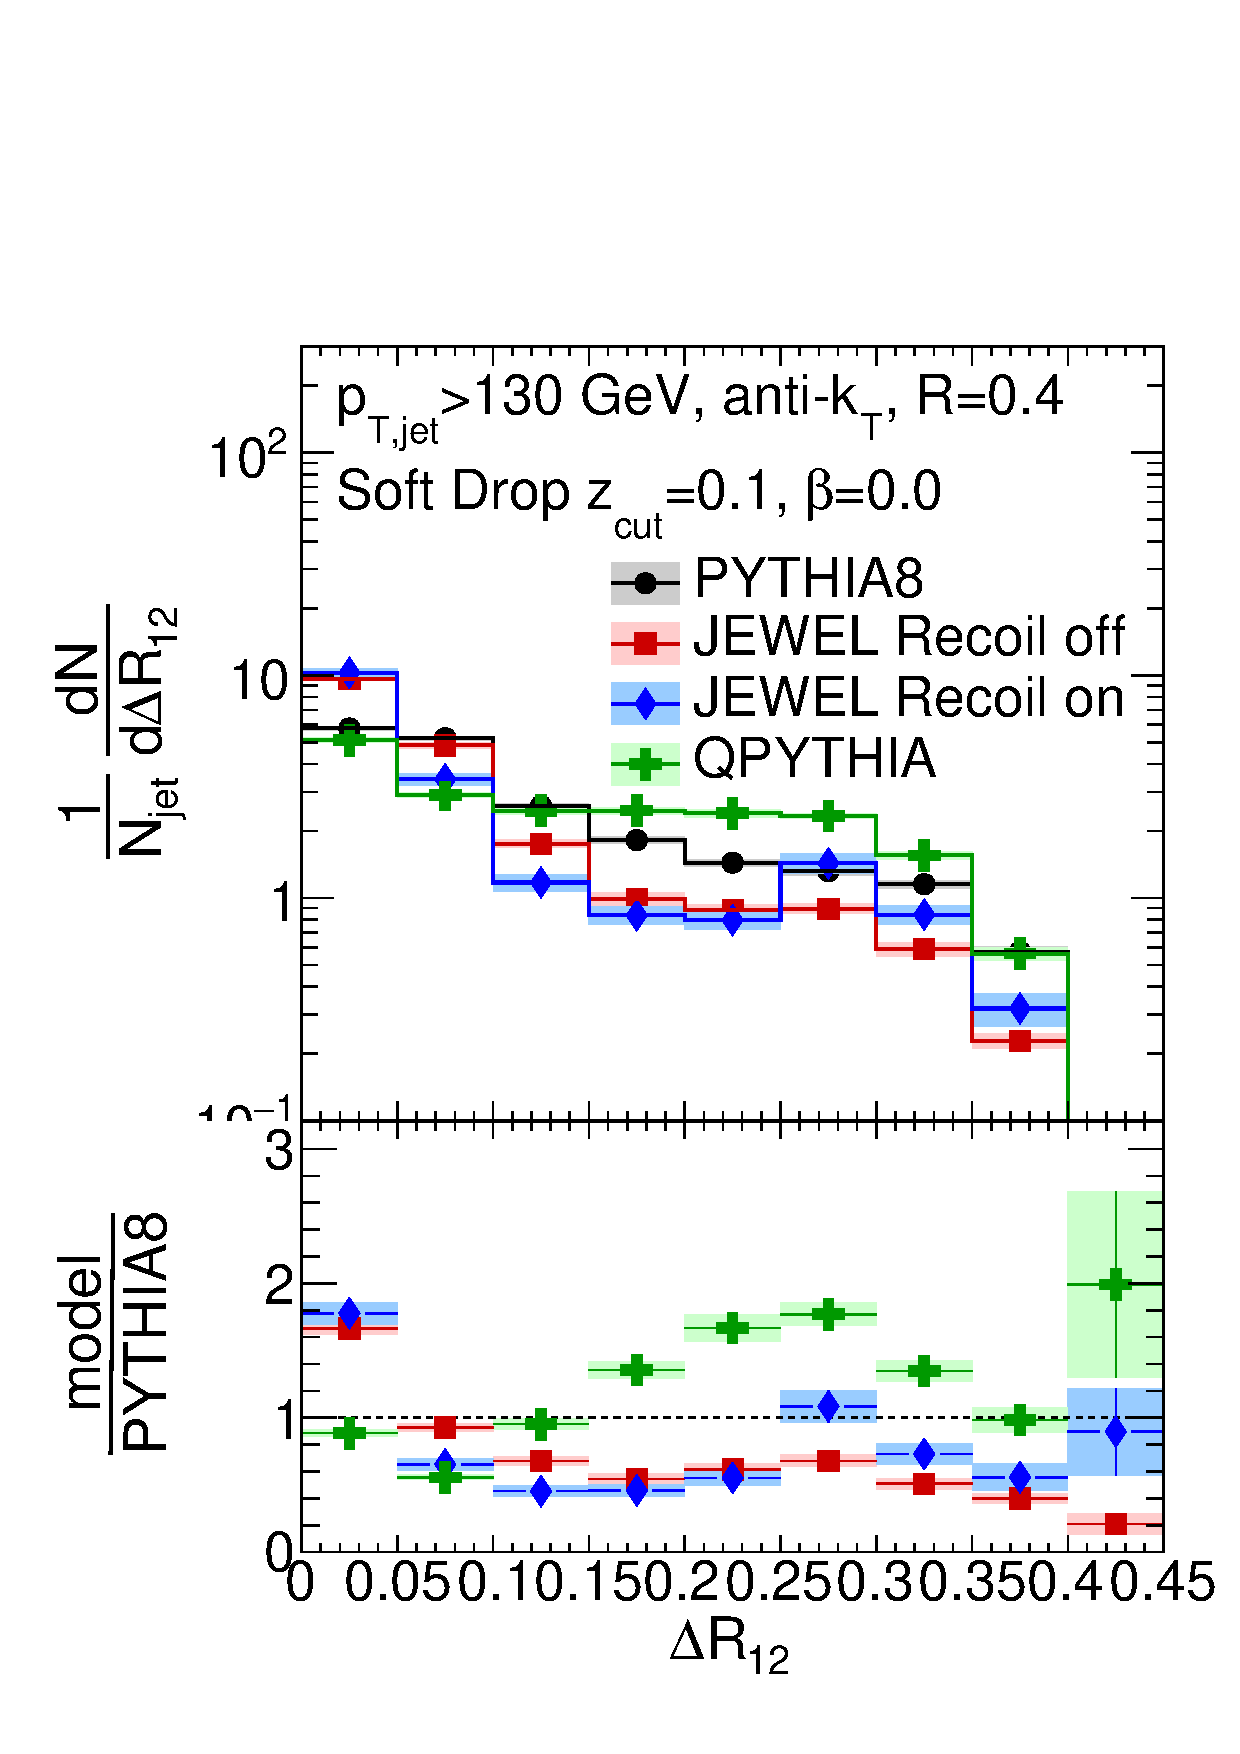
\includegraphics[width=0.33\textwidth]{figures/SDGen/DR12CompModelsBeta00Z01.pdf}%
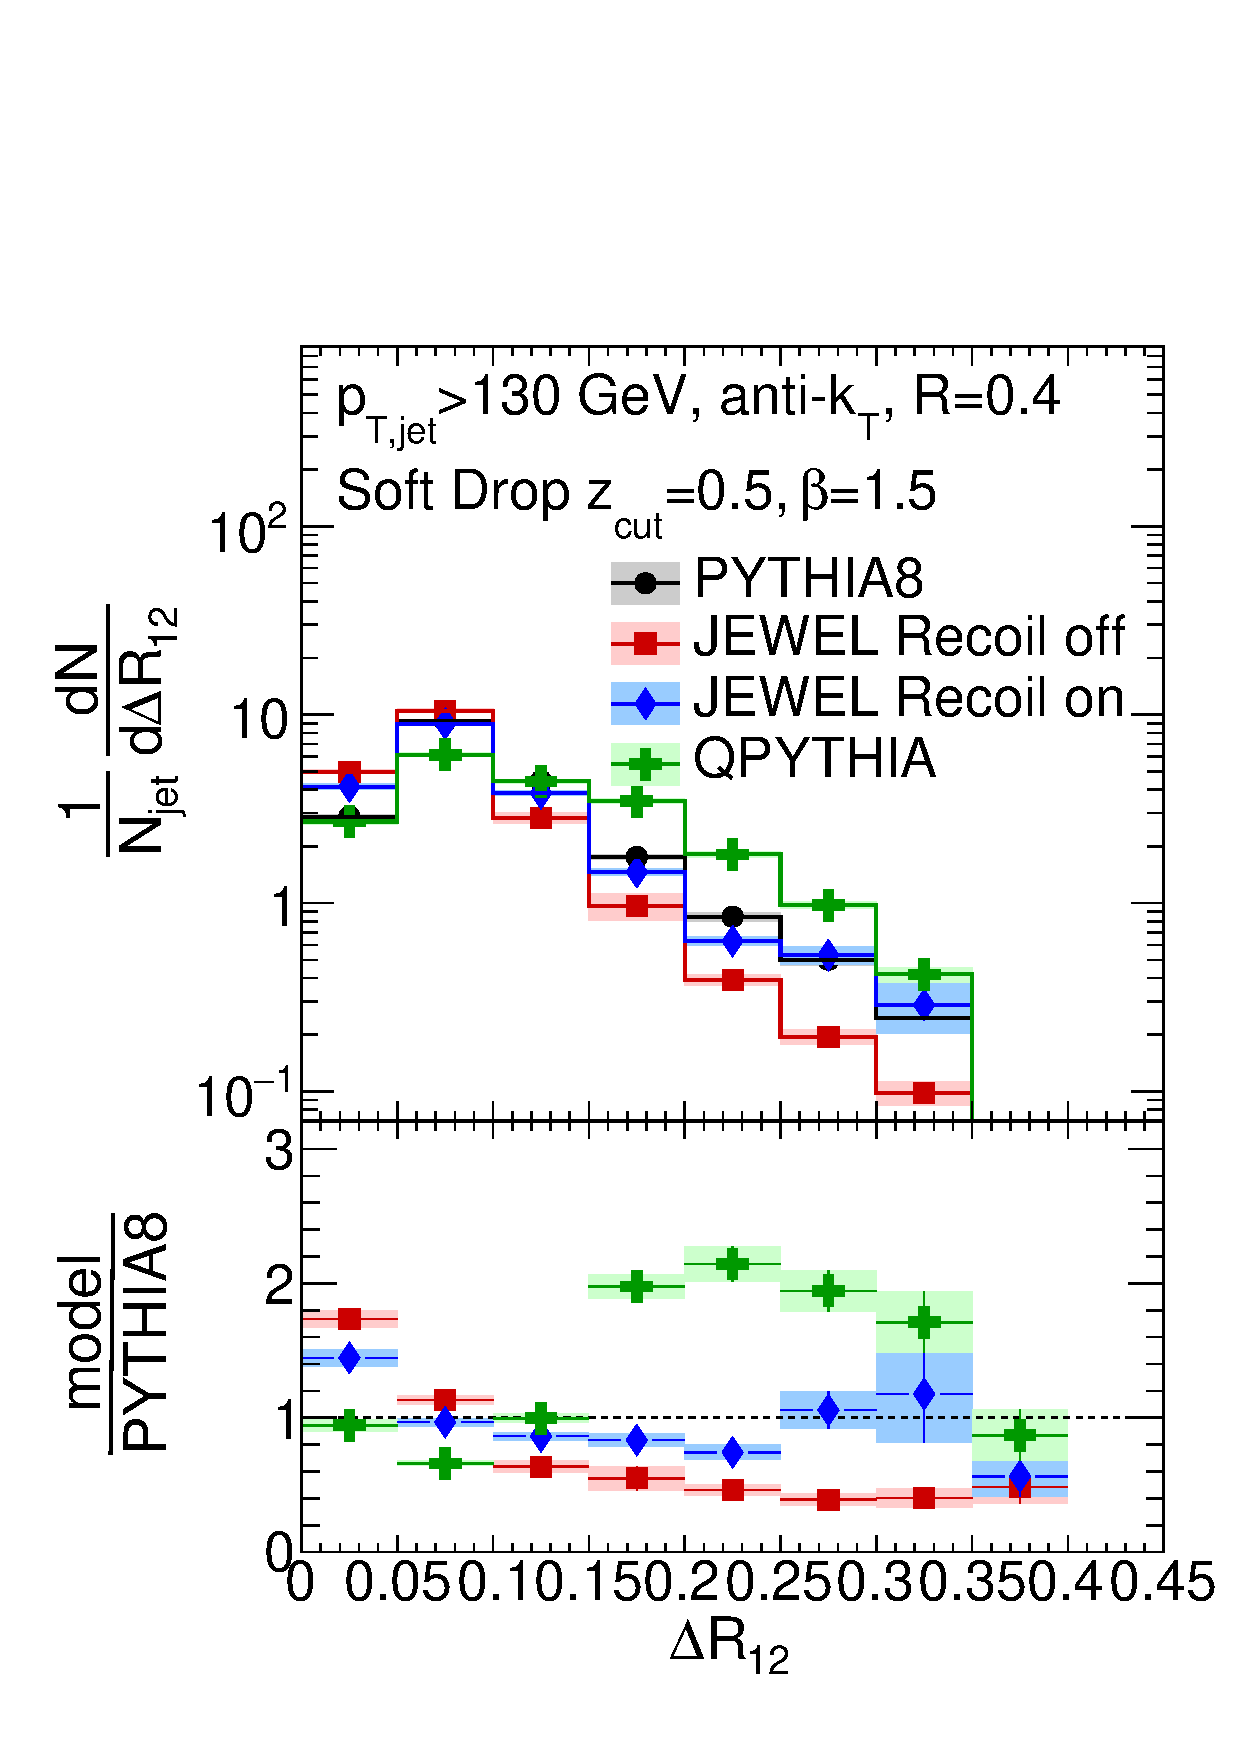
\includegraphics[width=0.33\textwidth]{figures/SDGen/DR12CompModelsBeta15Z05.pdf}%
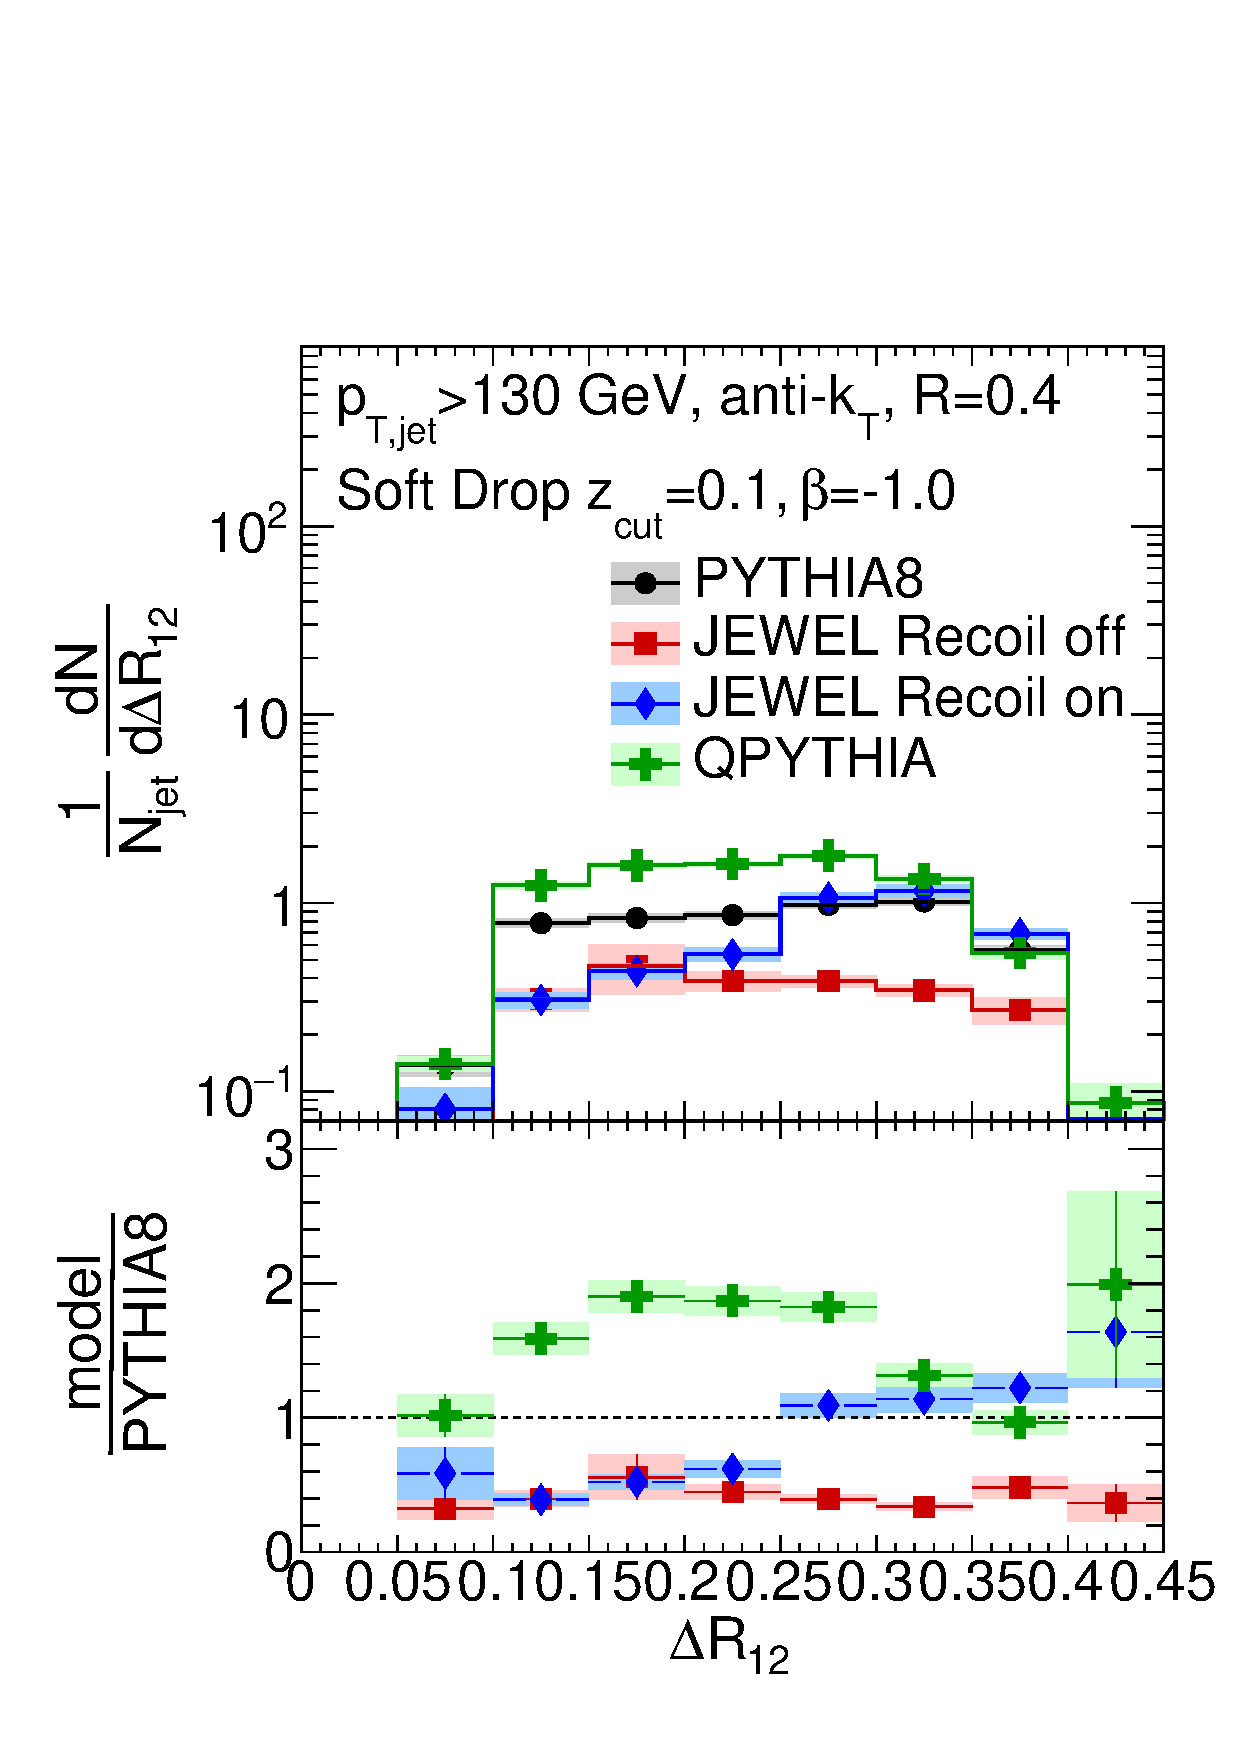
\includegraphics[width=0.33\textwidth]{figures/SDGen/DR12CompModelsBetam1Z01.pdf}%
\caption{Distance between the two groomed subjets, $\Delta R_{12}$, for three different grooming settings in simulations with and without jet quenching. The uppers panels show the $\Delta R_{\mathrm{12}}$ distribution normalized by the total number of ungroomed jets while the lower panels show the ratio of JEWEL and QPYTHIA with respect to PYTHIA8.}
\label{fig:SDGenDR12}
\end{figure}
%%%%%%%%%%%%%%%%%%%%%%%%%%%%%%%%%%%%%
Next we turn to studying the angular separation $\Delta R_{12}$ distribution of the groomed subjets. In the context of jet quenching, one particularly interesting question is to gauge whether substructures are quenched relative to their angular separation. The angular distance between the groomed sub-jets is plotted in \autoref{fig:SDGenDR12} for the three grooming settings. Once again, we see big differences between the MC models; JEWEL ``Recoils off'' being very collimated and QPYTHIA very broad. 
The JEWEL ``Recoils on'' setting interpolates between the two extremes and, most strikingly, exhibits an enhancement at intermediate angles, consistent with earlier studies of jet shape and fragmentation function \cite{KunnawalkamElayavalli:2017hxo}.

Once again, it is interesting to point out that the modifications are arguably the strongest for the most conservative SD setting, see \autoref{fig:SDGenDR12} (right). In particular, the JEWEL ``Recoils off'' samples are consistently suppressed for all angles. This could point to the importance of energy-loss that is not very sensitive to angle in JEWEL. The enhancement seen at small $\Delta R_{12}$ for $\beta \geq 0$, see \autoref{fig:SDGenDR12} (left, center), could also indicate a similar mechanism related to migration of narrow jets from higher $\pT$.
%The effect in JEWEL primarily shows up at large angels for all explored grooming settings. 
%In the JEWEL samples with $\beta \geq 0$ one observes larger sensitivity to recoil effects than for $\beta < 0$, which is remarkably flat for a wide range of angles.

%We note, in particular, a strong resilience to recoil effects in the JEWEL samples for all SD settings. Due to the suppression of large-angle jet structures in JEWEL (collimation), the small $M_g$ region is significantly enhanced compared to the vacuum baseline. 

%{\color{red} An interesting feature is perhaps that JEWEL is modified for small $M_g$ which technically implies that the splitting takes place outside of the medium. This is of course related to the enhancement seen at very small $\Delta R_{12}$. What is the reason for this modification? QPYTHIA is not modified there.}
%%%%%%%%%%%%%%%%%%%%%%%%%%%%%%%%%%%%%
\begin{figure}[th]
\centering
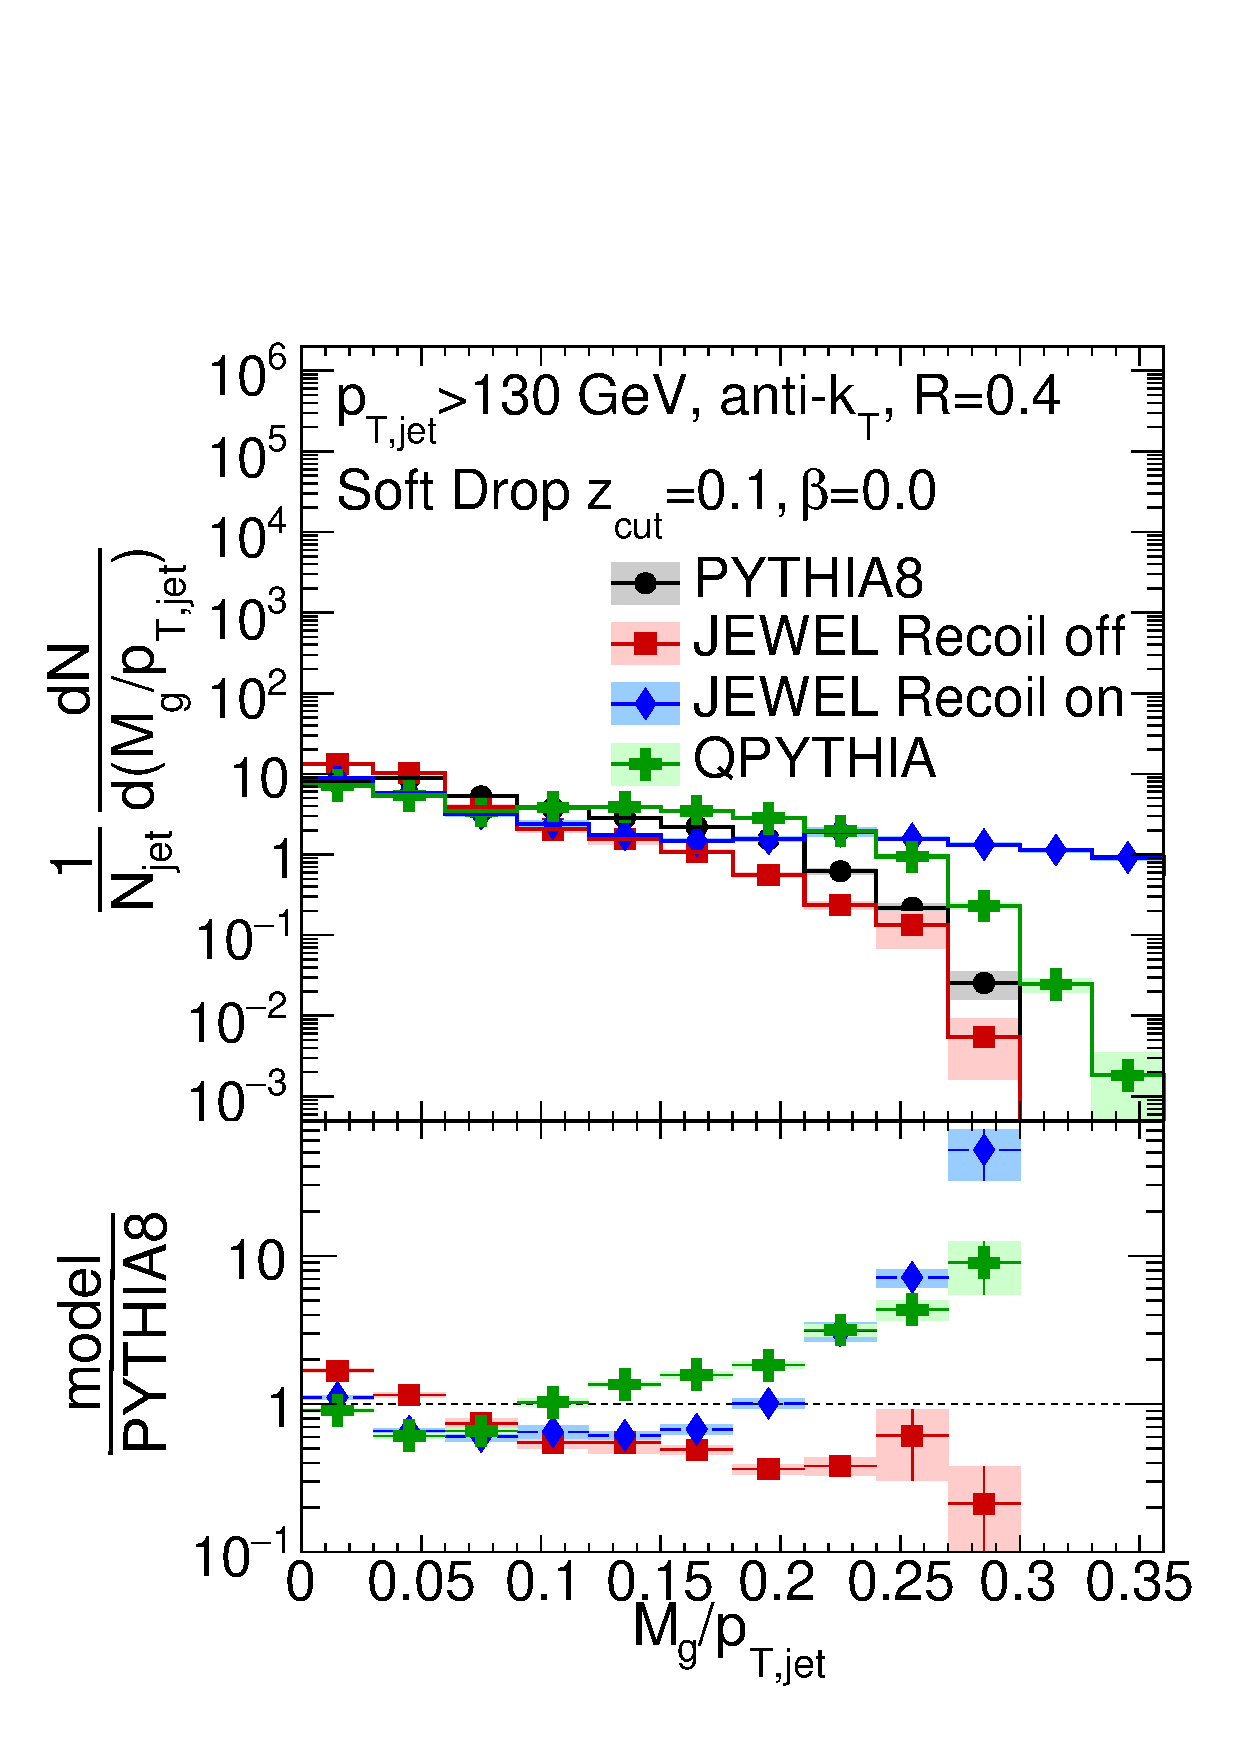
\includegraphics[width=0.33\textwidth]{figures/SDGen/MgOverPtgCompModelsBeta00Z01.pdf}%
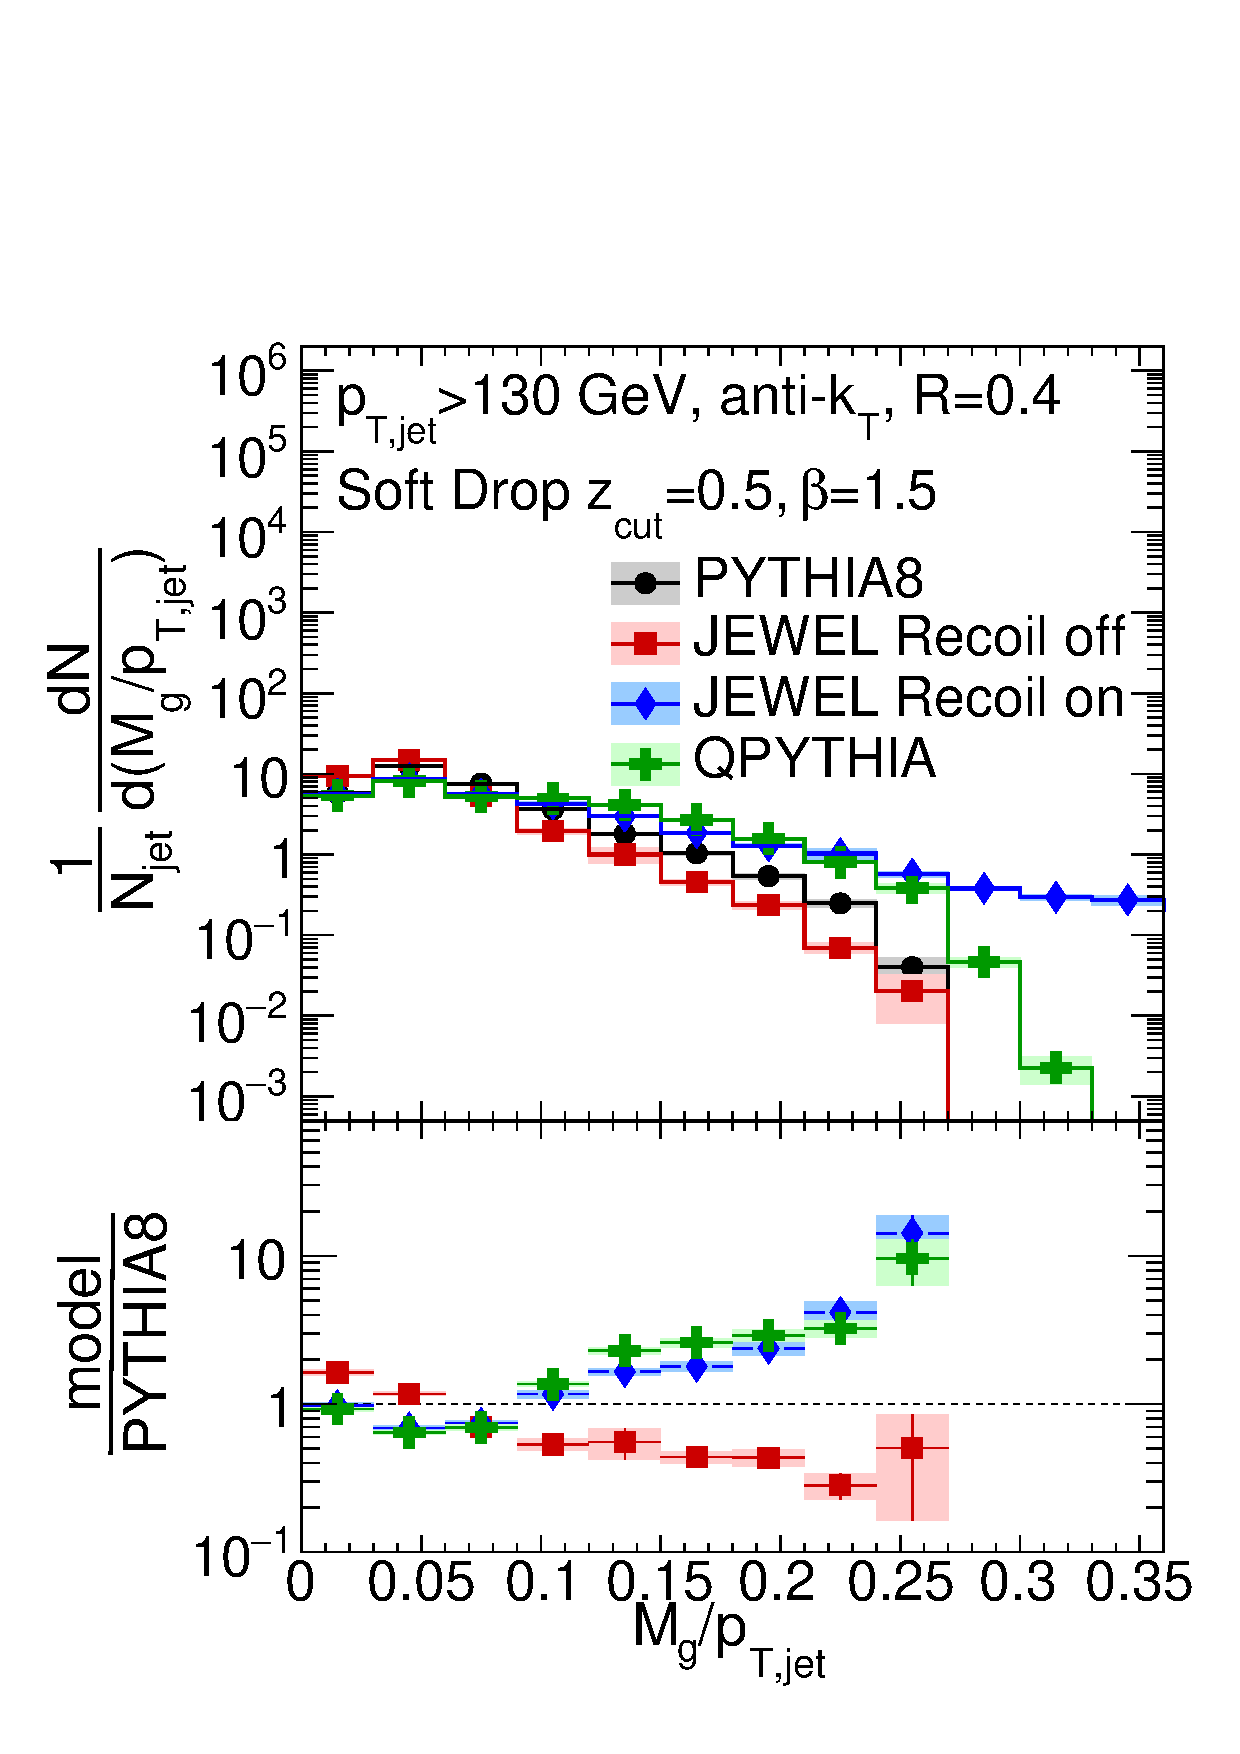
\includegraphics[width=0.33\textwidth]{figures/SDGen/MgOverPtgCompModelsBeta15Z05.pdf}%
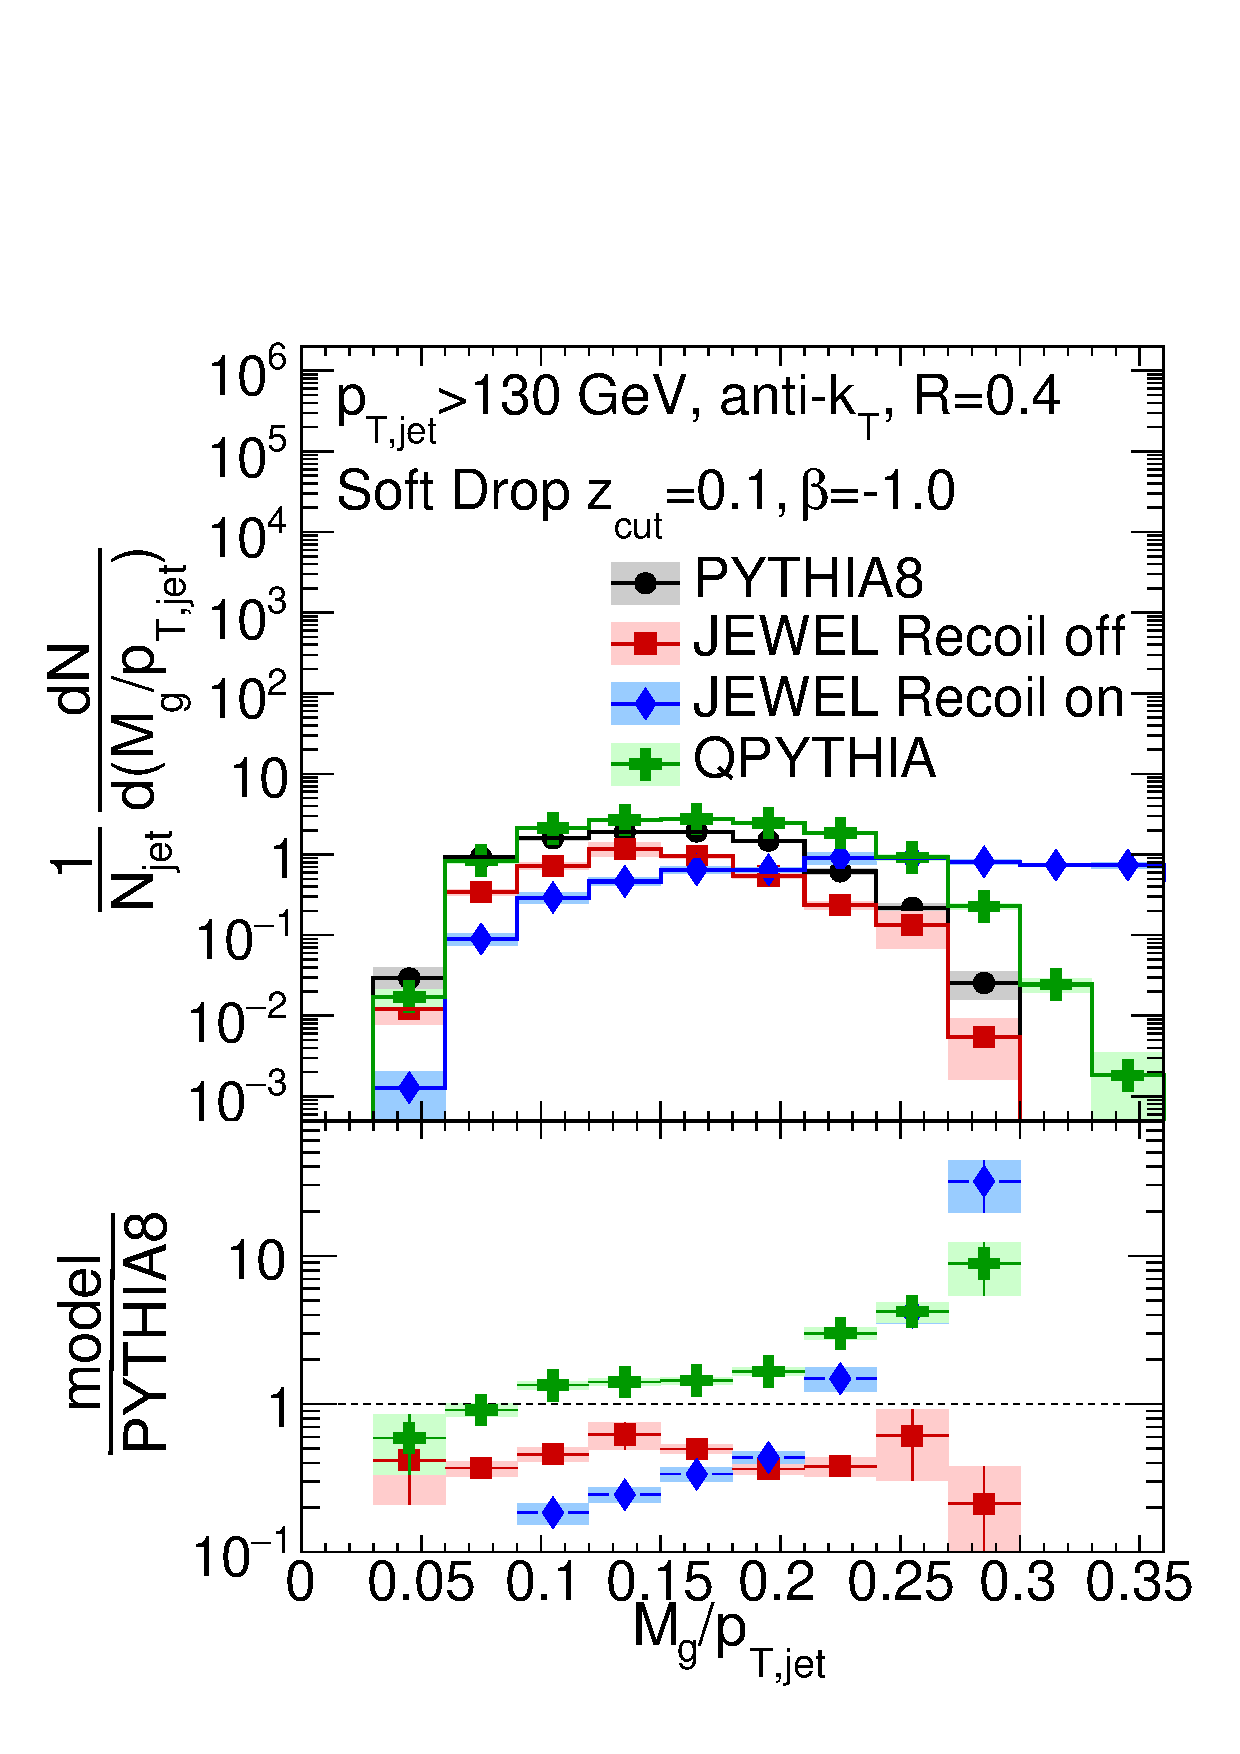
\includegraphics[width=0.33\textwidth]{figures/SDGen/MgOverPtgCompModelsBetam1Z01.pdf}%
\caption{Groomed jet mass, $M_{\mathrm{g}}/p_{\mathrm{T,jet}}$, for three different grooming settings in simulations with and without jet quenching. The uppers panels show the $M_{\mathrm{g}}/p_{\mathrm{T,jet}}$ distribution normalized by the total number of ungroomed jets while the lower panels show the ratio of JEWEL and QPYTHIA with respect to PYTHIA8.
%\kmt{Yi: gen-level makes sense, with embedding mass gets enhanced.}
}
\label{fig:SDGenMg}
\end{figure}
%%%%%%%%%%%%%%%%%%%%%%%%%%%%%%%%%%%%%
Finally, we study the groomed jet mass normalized by the transverse momentum, $M_{\mathrm{g}}/p_{\mathrm{T,jet}}$, in \autoref{fig:SDGenMg}. 
This observable combines several of the features already seen before and seems particularly constraining of large-mass jet substructures. In this case, the QPYTHIA and JEWEL ``Recoils on'' samples give rise to similar distributions with a strong enhancement at large $M_g/\pT$. The enhancement is the largest for the latter model. In contrast, JEWEL ``Recoils off'' is more resilient and exhibits a mild suppression with respect to vacuum results at high-masses. This could again be interpreted as an effect of energy-loss.
During the preparation of the workshop report results on the groomed mass in heavy-ion collisions at the LHC was released by the CMS collaboration \cite{Sirunyan:2018gct}. 

To summarize, these generator level studies of the kinematics of the subjet samples obtained using Soft Drop illustrates the wide range of sensitivity to different kinematical regimes, and therefore different effects. Further studies, including embedding and involving more medium models, are planned for the future and could help further constrain large classes of medium effects.

%%\clearpage
%%\newpage
%%%%%%%%%%%%%%%%%%%%%%%%%%%%%%%%%%%%%%%%%%
%\subsection{Sensitivity to reclustering algorithm} {\color{green} Leticia, Harry}
%\label{sec:reclusteringalgo}
%%%%%%%%%%%%%%%%%%%%%%%%%%%%%%%%%%%%%%%%%%
%The strategy of the clustering algorithm manifests itself in the declustering and grooming. CA algorithm combines the closest particles first. As a consequence, the first declustering steps will encounter soft splittings at large angle. In the case of k$_{T}$ algorithm, the softest particles are clustered first. As a consequence, the first declustering steps will encounter hard splittings. Anti-k$_{T}$ clusters hard particles first, thus splittings at the first declustering steps will be generally soft. Such ordering is reflected in the Lund plots of \autoref{fig:AlgoDependence}.
%\begin{figure}[th]
%\centering
%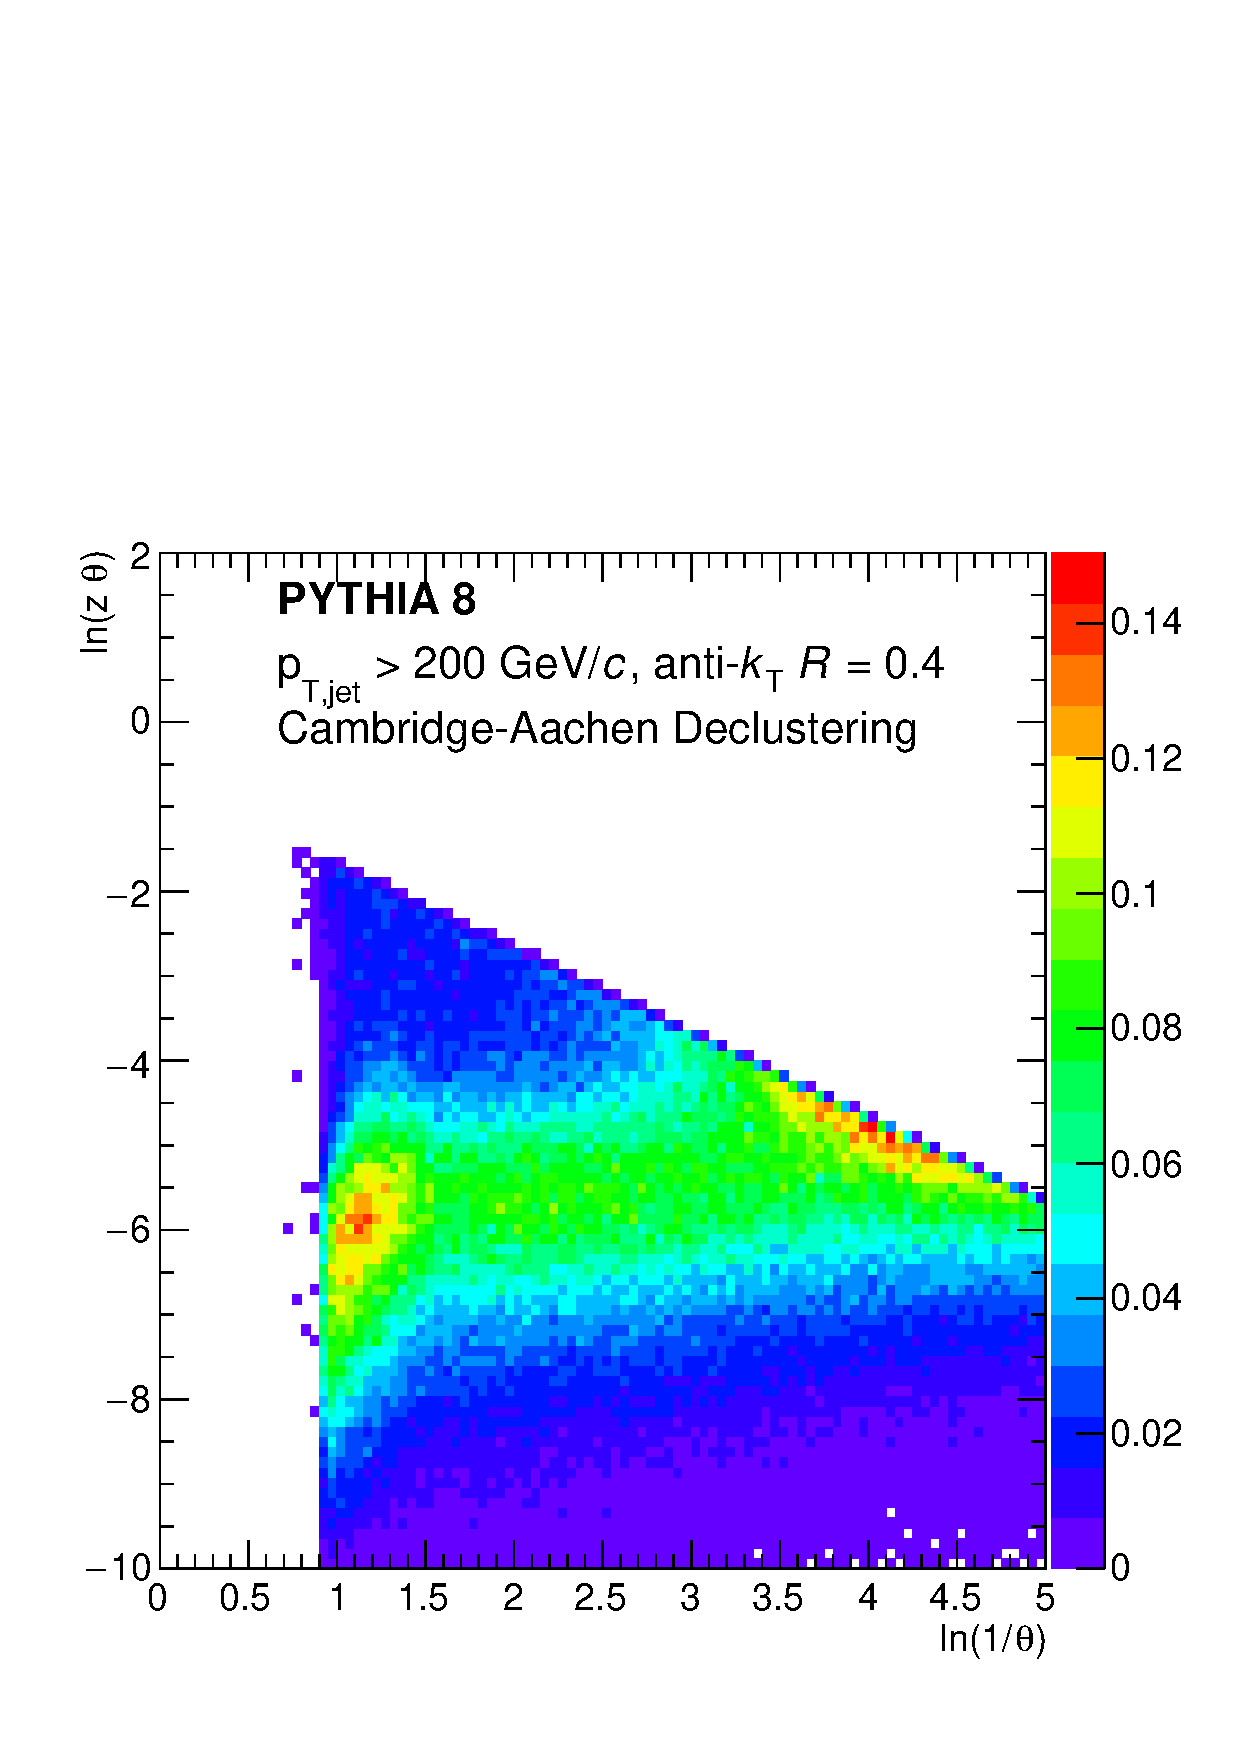
\includegraphics[width=0.33\textwidth]{figures/LundMC/Pythia_CA.pdf}%
%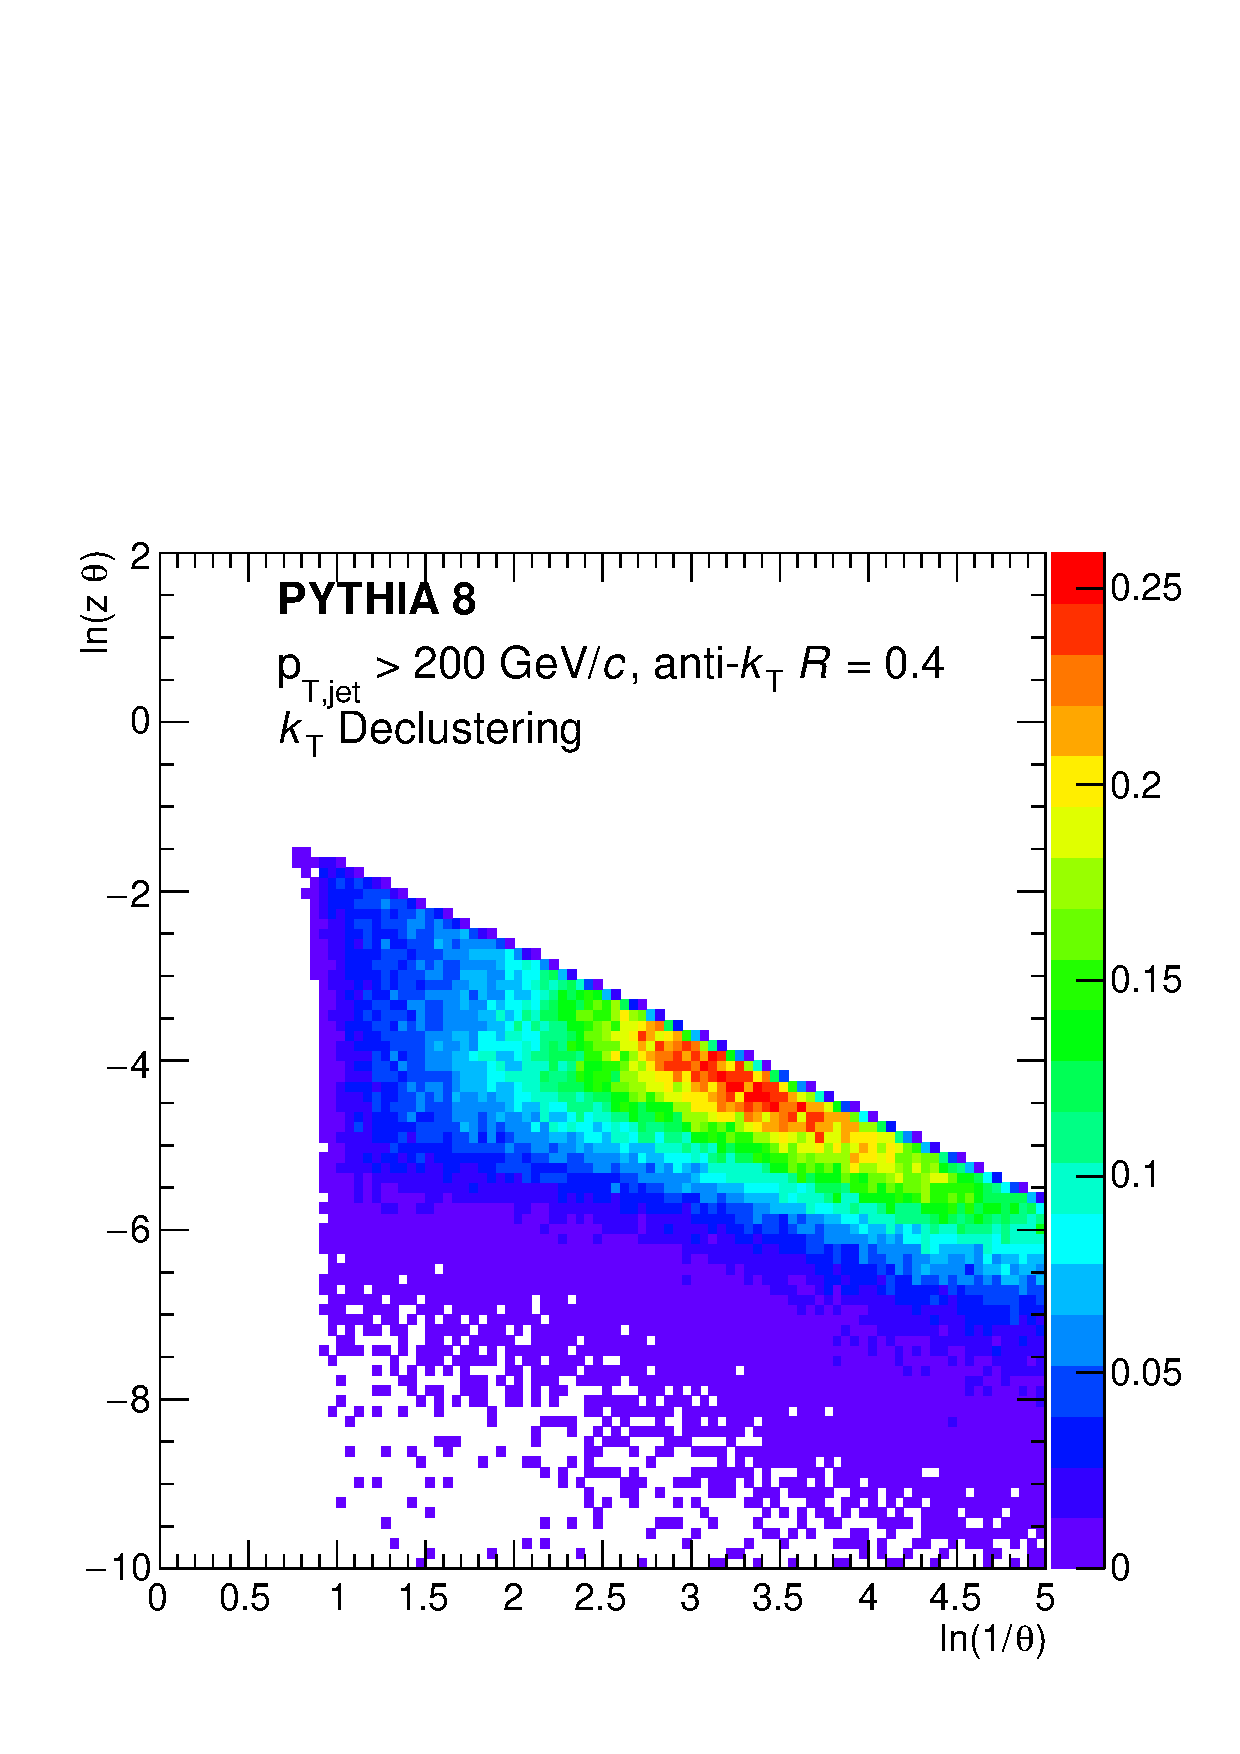
\includegraphics[width=0.33\textwidth]{figures/LundMC/Pythia_kt.pdf}%
%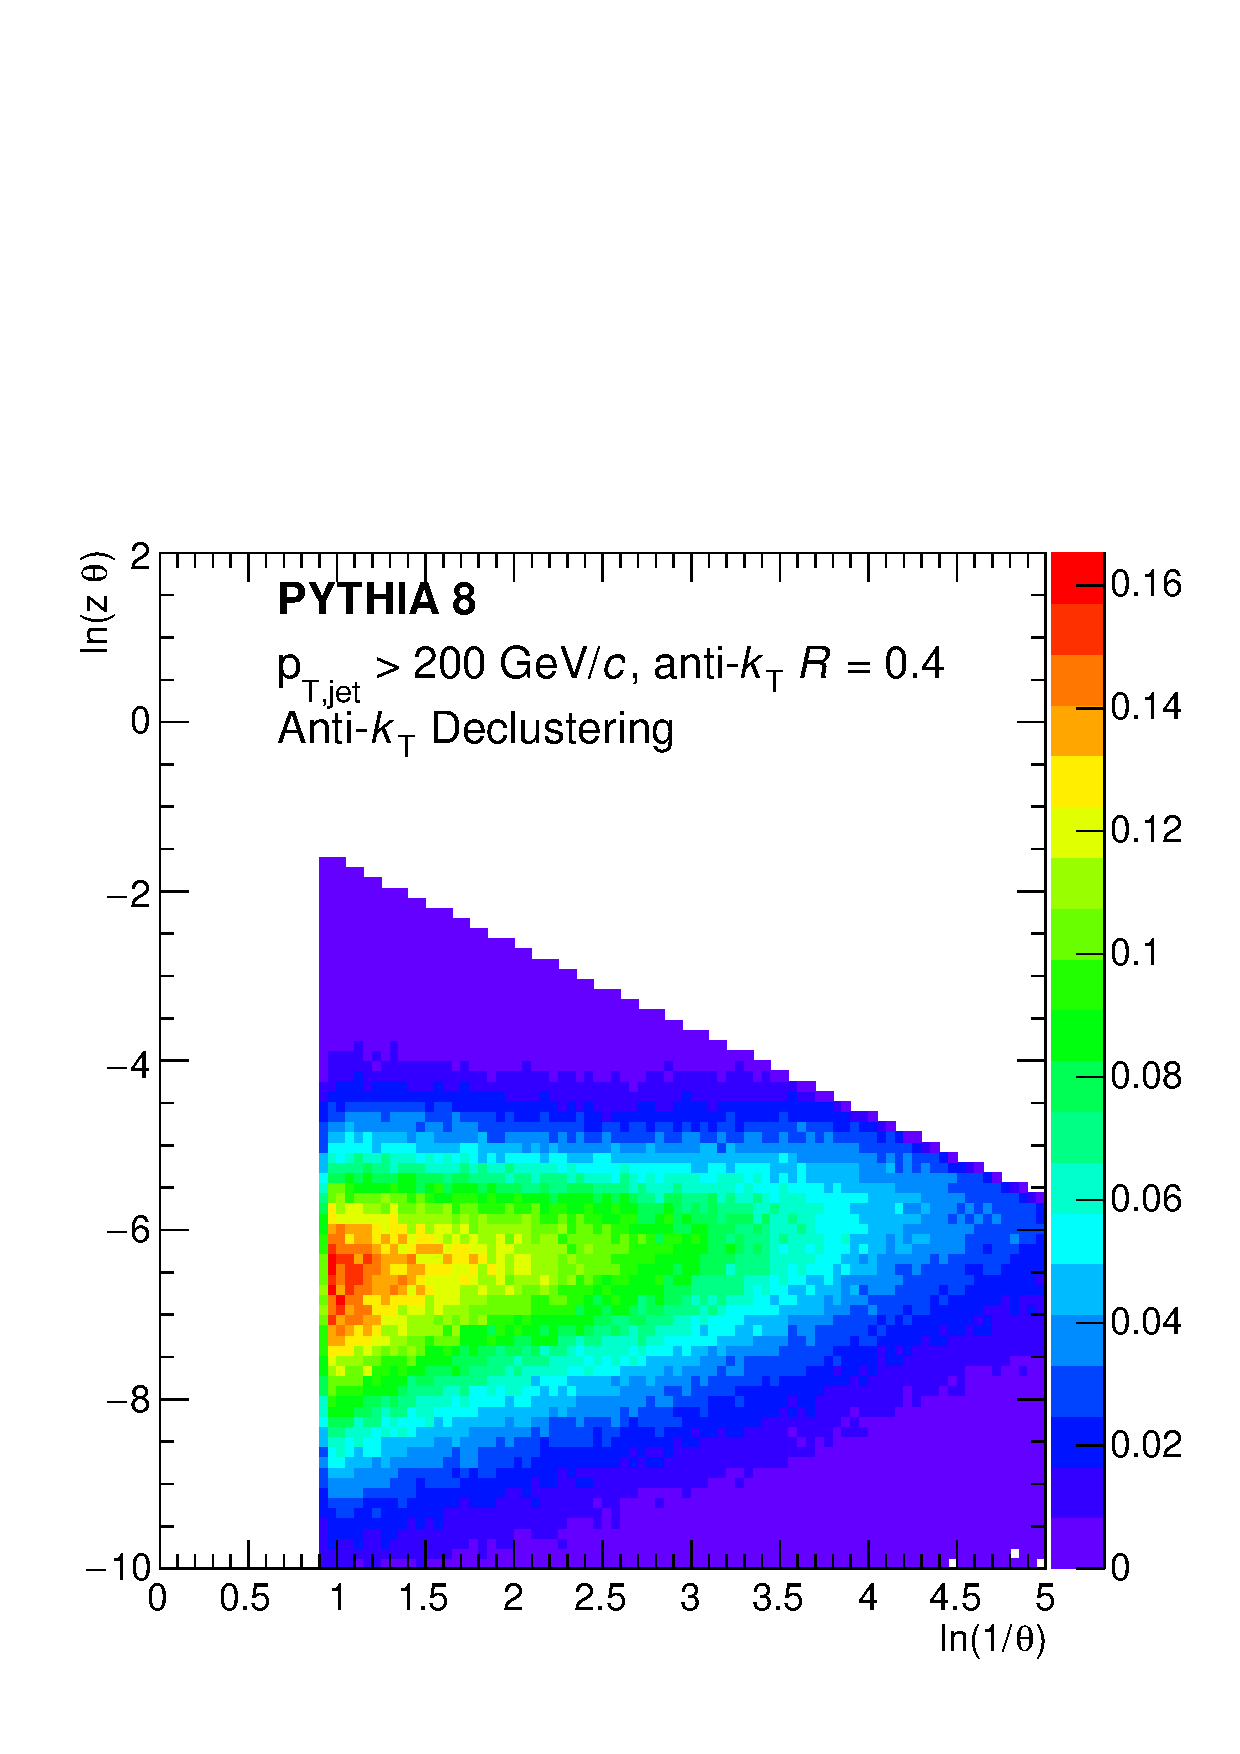
\includegraphics[width=0.33\textwidth]{figures/LundMC/Pythia_Akt.pdf}%
%\caption{Lund plot for different declustering strategies: CA (left), k$_{T}$(middle), Anti-k$_{T}$ (right)}
%\label{fig:AlgoDependence}
%\end{figure}
%
%
%In Fig. \ref{fig:AlgoDependenceSignal}, left plot, the difference between JEWEL (recoils off) and vacuum is shown for k$_{T}$ declustering strategy. The similar plot for QPYTHIA is shown on the right plot. We see that in the case of JEWEL, the excess of splittings at large angle is of the same order of magnitude with CA and k$_{T}$ strategies and around 20 $\%$. In the case of QPYTHIA, the excess of splittings at large $k_{T}$ is enhanced to 20$\%$ with k$_{T}$ strategy compared to the 8$\%$ enhancement we observe for CA strategy in Fig. \ref{fig:PS2Vac} lower left plot. 
%
%
%\begin{figure}[th]
%\centering
%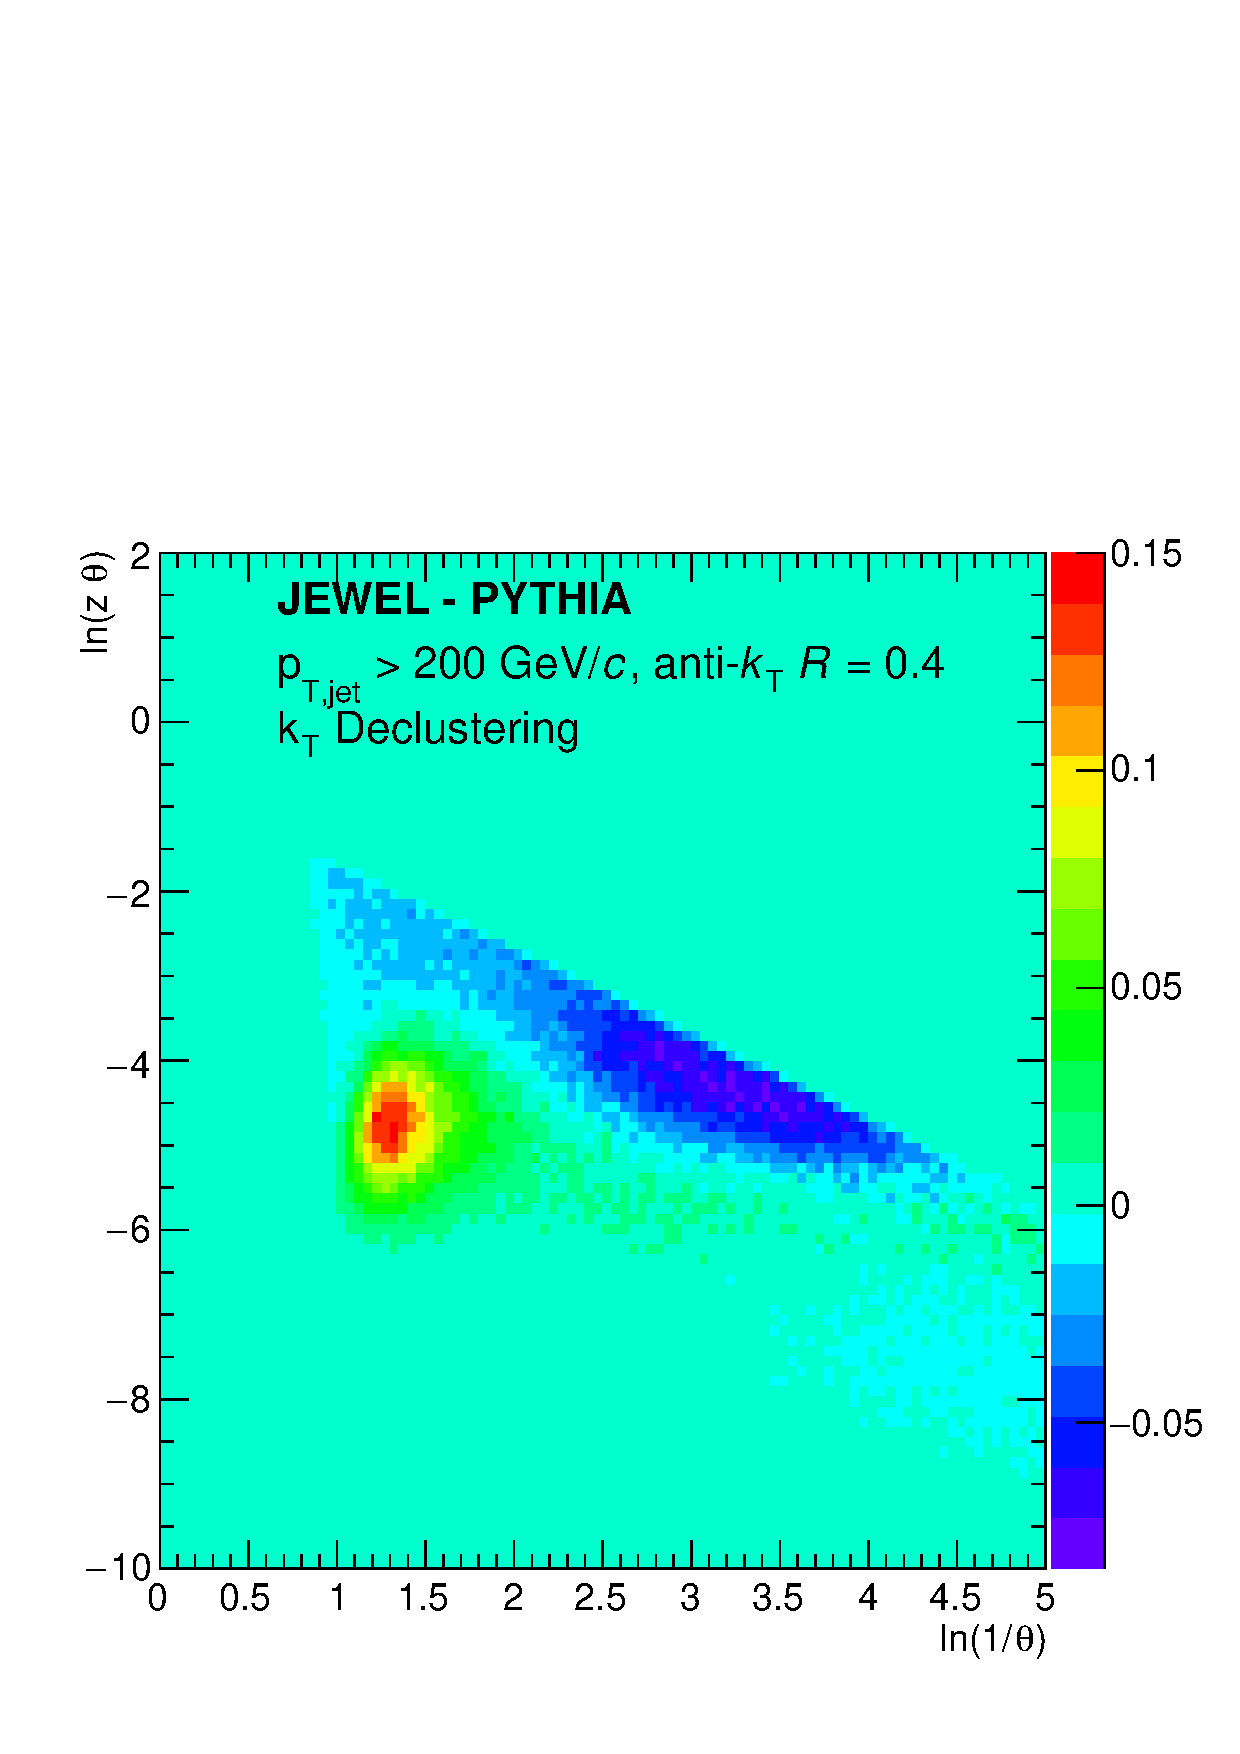
\includegraphics[width=0.33\textwidth]{figures/LundMC/SignalGeneratorDiff_kt.pdf}%
%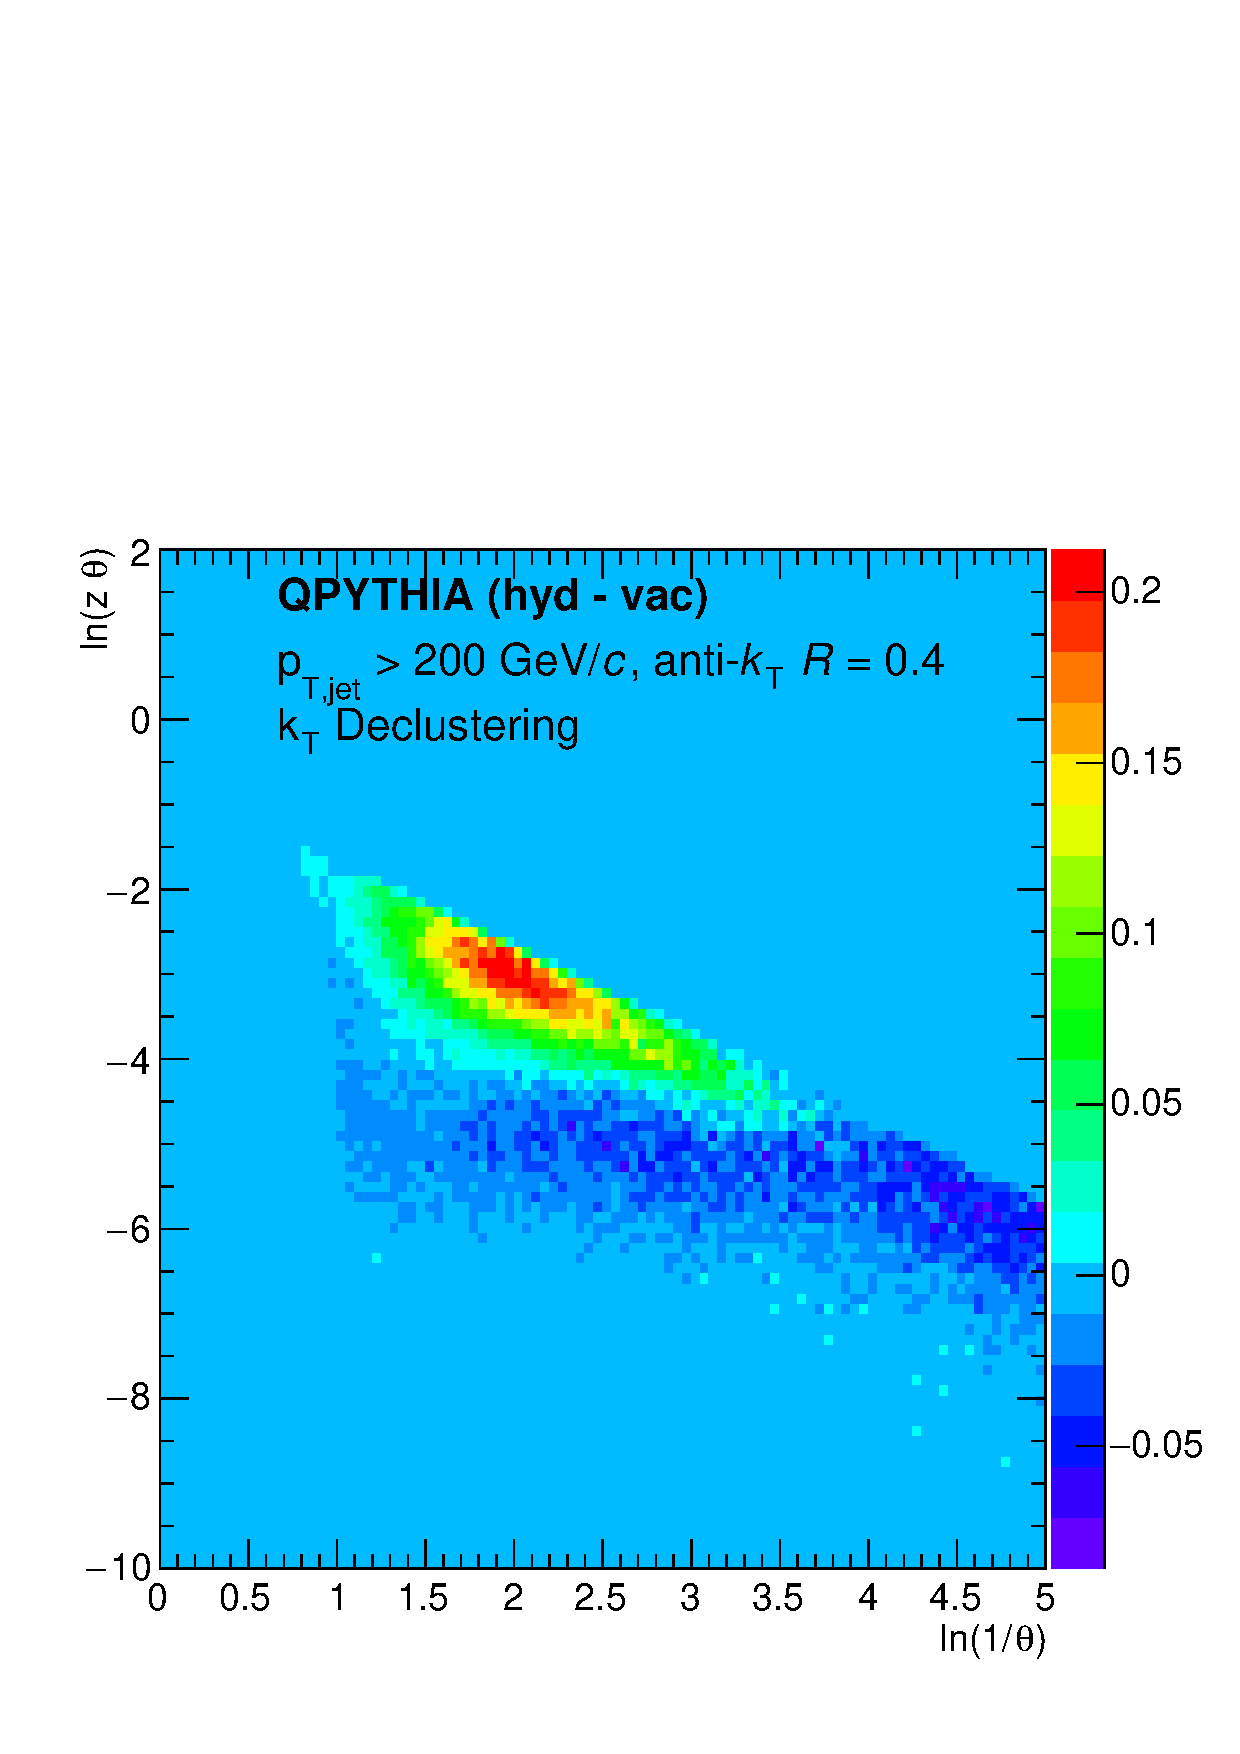
\includegraphics[width=0.33\textwidth]{figures/LundMC/QPythiaDiff_kt.pdf}%
%\caption{Difference of radiation pattern of JEWEL (no recoils) relative to vacuum using k$_{T}$ strategy (left). Same plot for QPYTHIA (right)}
%\label{fig:AlgoDependenceSignal}
%\end{figure}
%
%
%%%%%%%%%%%%%%%%%%%%%%%%%%%%%%%%%%%%%%%%%
\subsubsection{Sensitivity to hadronization effects}
\label{sec:hadronization}
%%%%%%%%%%%%%%%%%%%%%%%%%%%%%%%%%%%%%%%%%


The last stage of the jet fragmentation is the non-perturbative process of hadronization. This is a dynamical process that converts colored partons into color-singlet hadrons. In jet quenching event generators it is typically assumed that hadronization occurs outside of the medium. A proof for this assumption does not exist and therefore hadronization uncertainties should be expected to be sizable. 

%%%%%%%%%%%%%%%%%%%%%%%%%%%%%%%%%%%%%
\begin{figure}[th]
\centering
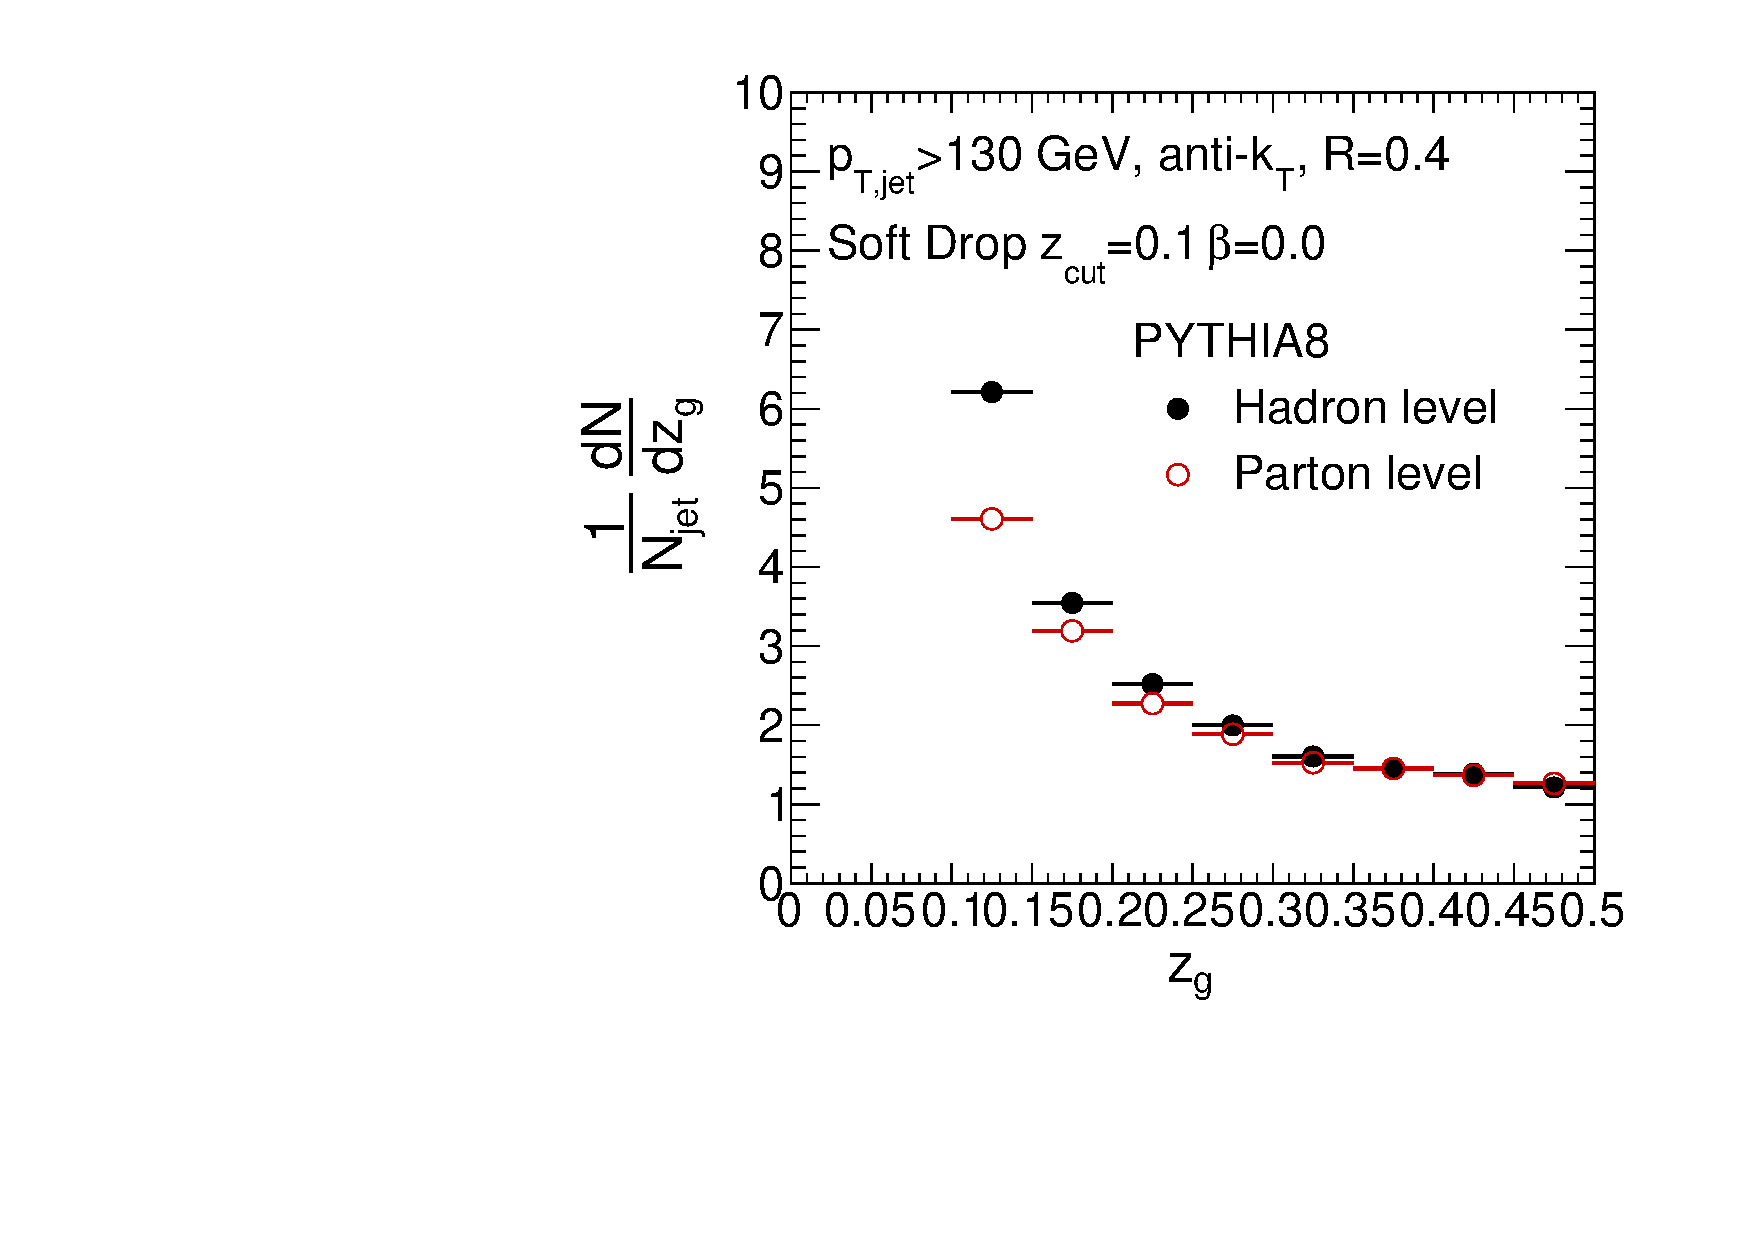
\includegraphics[width=0.33\textwidth]{figures/SDGen/ZgPytHadVsPartBeta00Z01.pdf}%
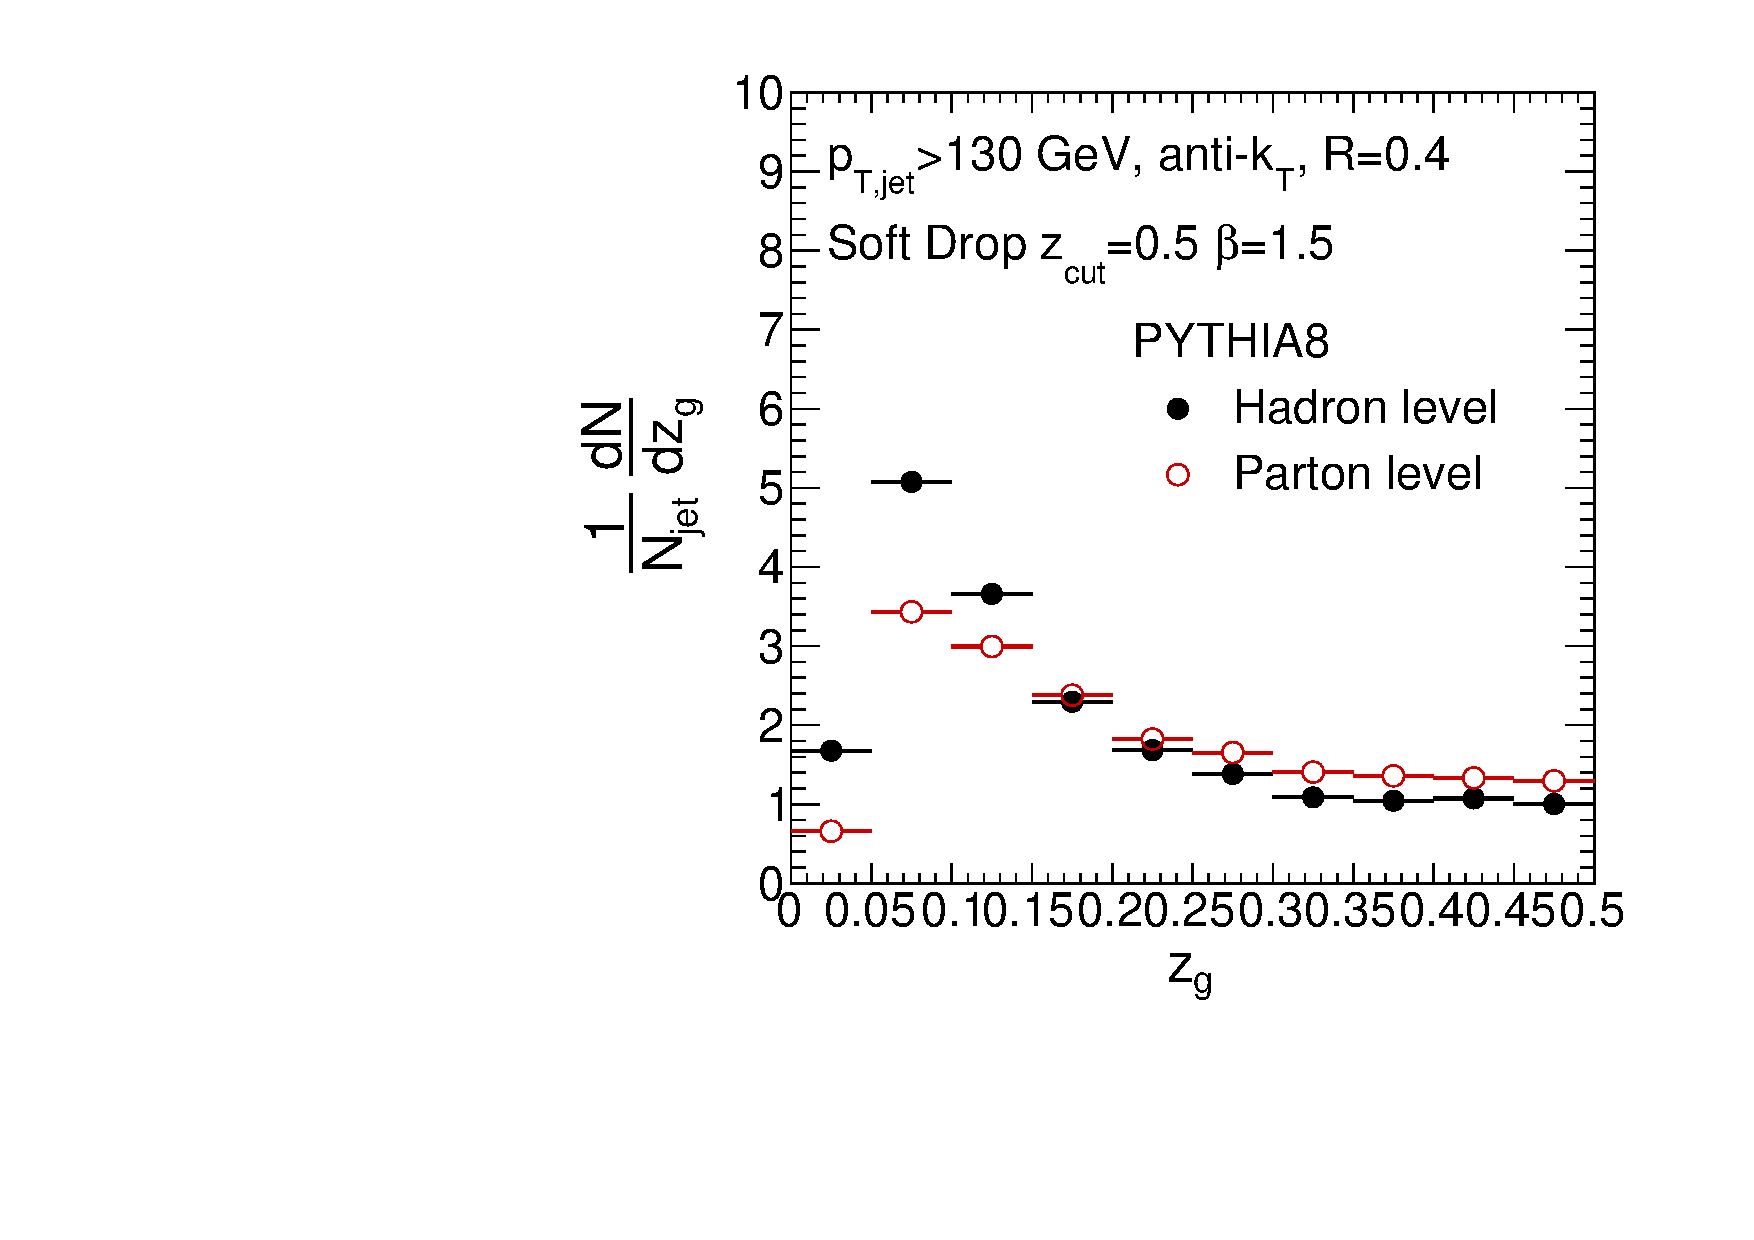
\includegraphics[width=0.33\textwidth]{figures/SDGen/ZgPytHadVsPartBeta15Z05.pdf}%
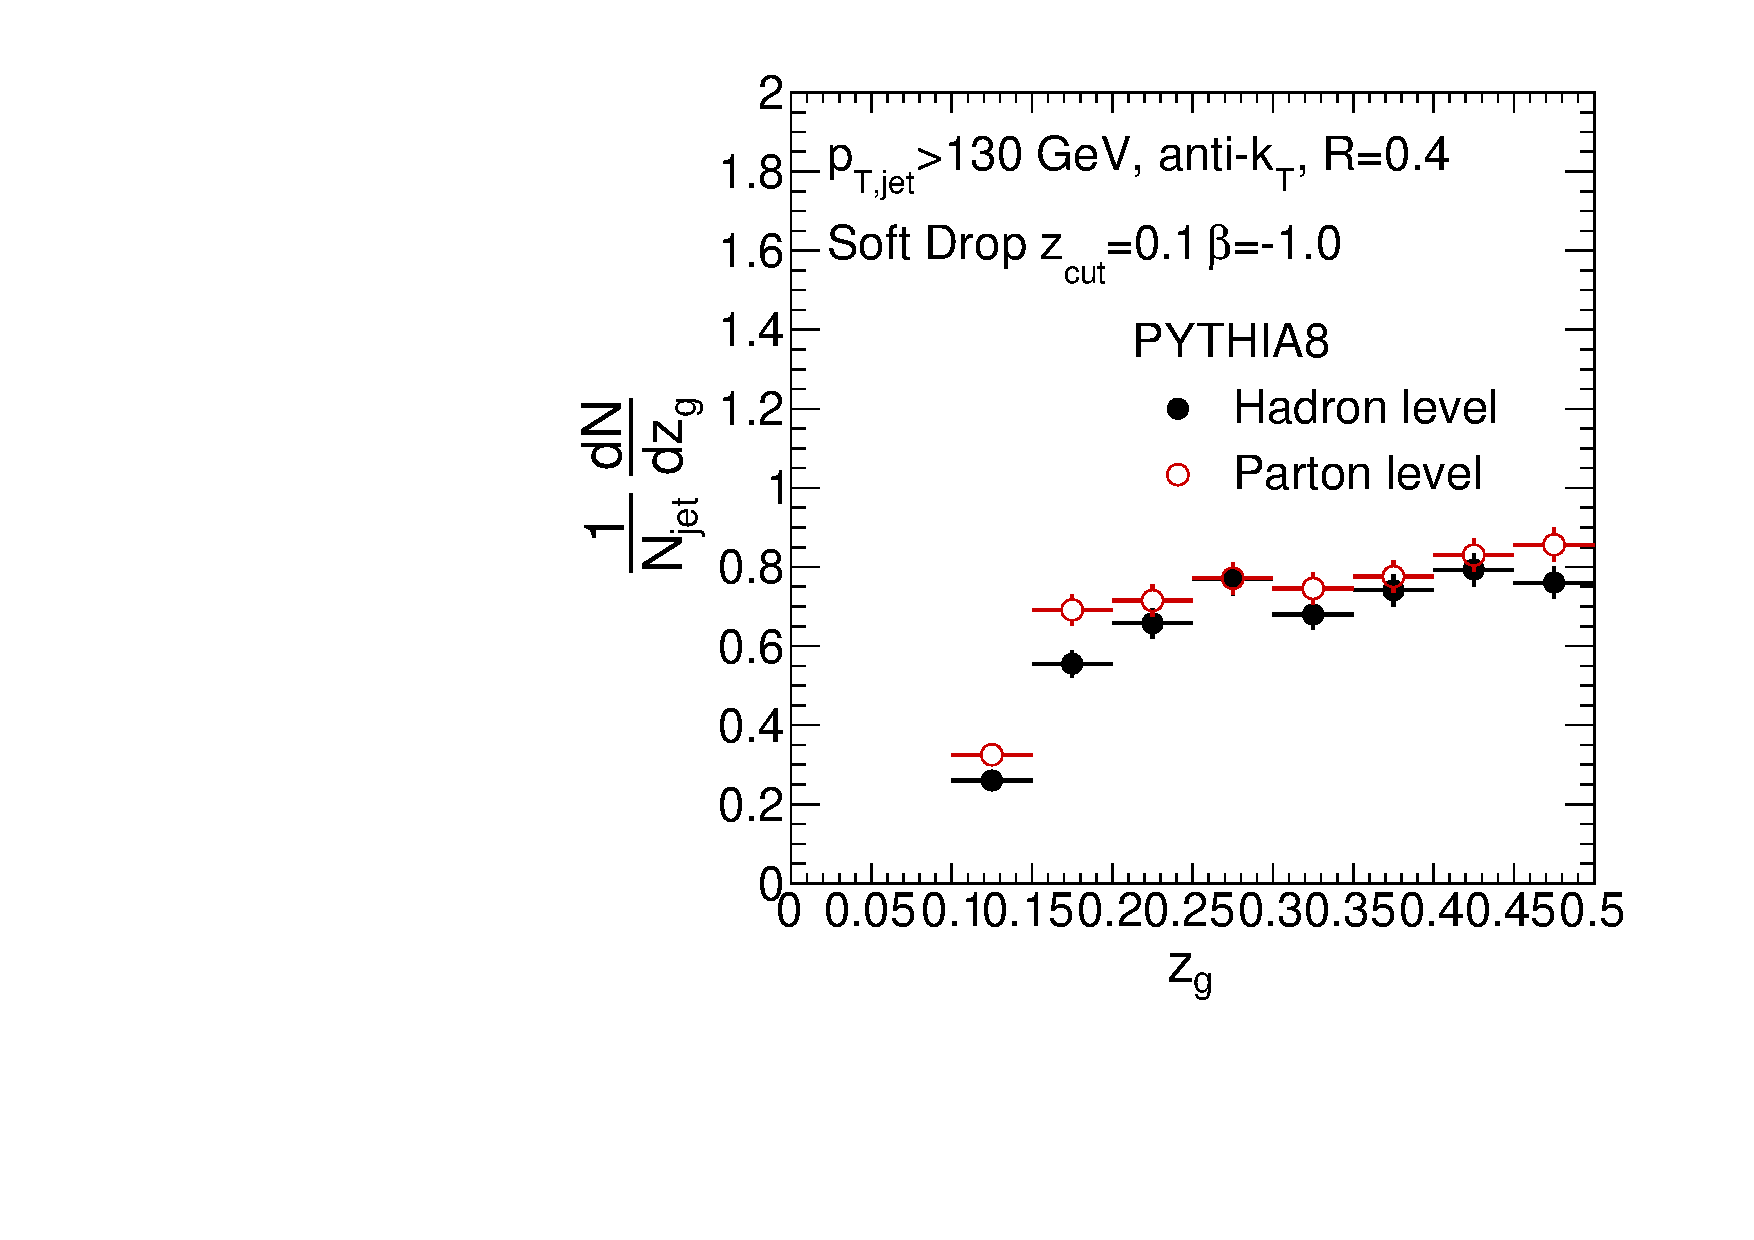
\includegraphics[width=0.33\textwidth]{figures/SDGen/ZgPytHadVsPartBetam1Z01.pdf}%
\caption{Groomed shared momentum fraction, $z_{\mathrm{g}}$, for three different grooming settings in simulations with and without hadronization with the PYTHIA8 event generator.}
\label{fig:SDGenZGHadVsPart}
\end{figure}
%%%%%%%%%%%%%%%%%%%%%%%%%%%%%%%%%%%%%
Even for vacuum physics, it is well known that the SD procedure has some sensitivity to hadronization effects, for $\beta = 0$ see \cite{Dasgupta:2015yua}.
From perturbative arguments hadronization corrections to the jet $p_{T}$ grow like $R^{-1}$ \cite{Dasgupta:2007wa} and
%inversely proportional to the jet resolution $R$: $\Delta p_{T}^{had} \approx \frac{-1}{R}$, 
so are potentially important for subjet observables.
However, since hadronization is a process that happens locally in phase space, jets are less sensitive to the hadronization uncertainties than observables based on hadrons. In this paragraph we investigate how sensitive groomed subjet observables are to the hadronization process. For this purpose we compare the \zg~distribution in PYTHIA8 with and without hadronization for the three SD settings described above, as shown in \autoref{fig:SDGenZGHadVsPart}. It can be observed that the low-\zg\, region is particularly sensitive to hadronization effects. For grooming with negative $\beta$ the hadron- and parton-level results are most similar, see Fig,~\ref{fig:SDGenZGHadVsPart} (right), because with these grooming settings the soft splittings are rejected. Dedicated studies of these effects in conjunction with medium-modified hadronization are left for the future.

%%%%%%%%%%%%%%%%%%%%%%%%%%%%%%%%%%%%%%%%%
\subsubsection{Issues with changing reclustering algorithm}
\label{sec:reclusteringalgo}
%%%%%%%%%%%%%%%%%%%%%%%%%%%%%%%%%%%%%%%%%

%%%%%%%%%%%%%%%%%%%%%%%%%%%%%%%%%%%%%
\begin{figure}[t!]
\centering
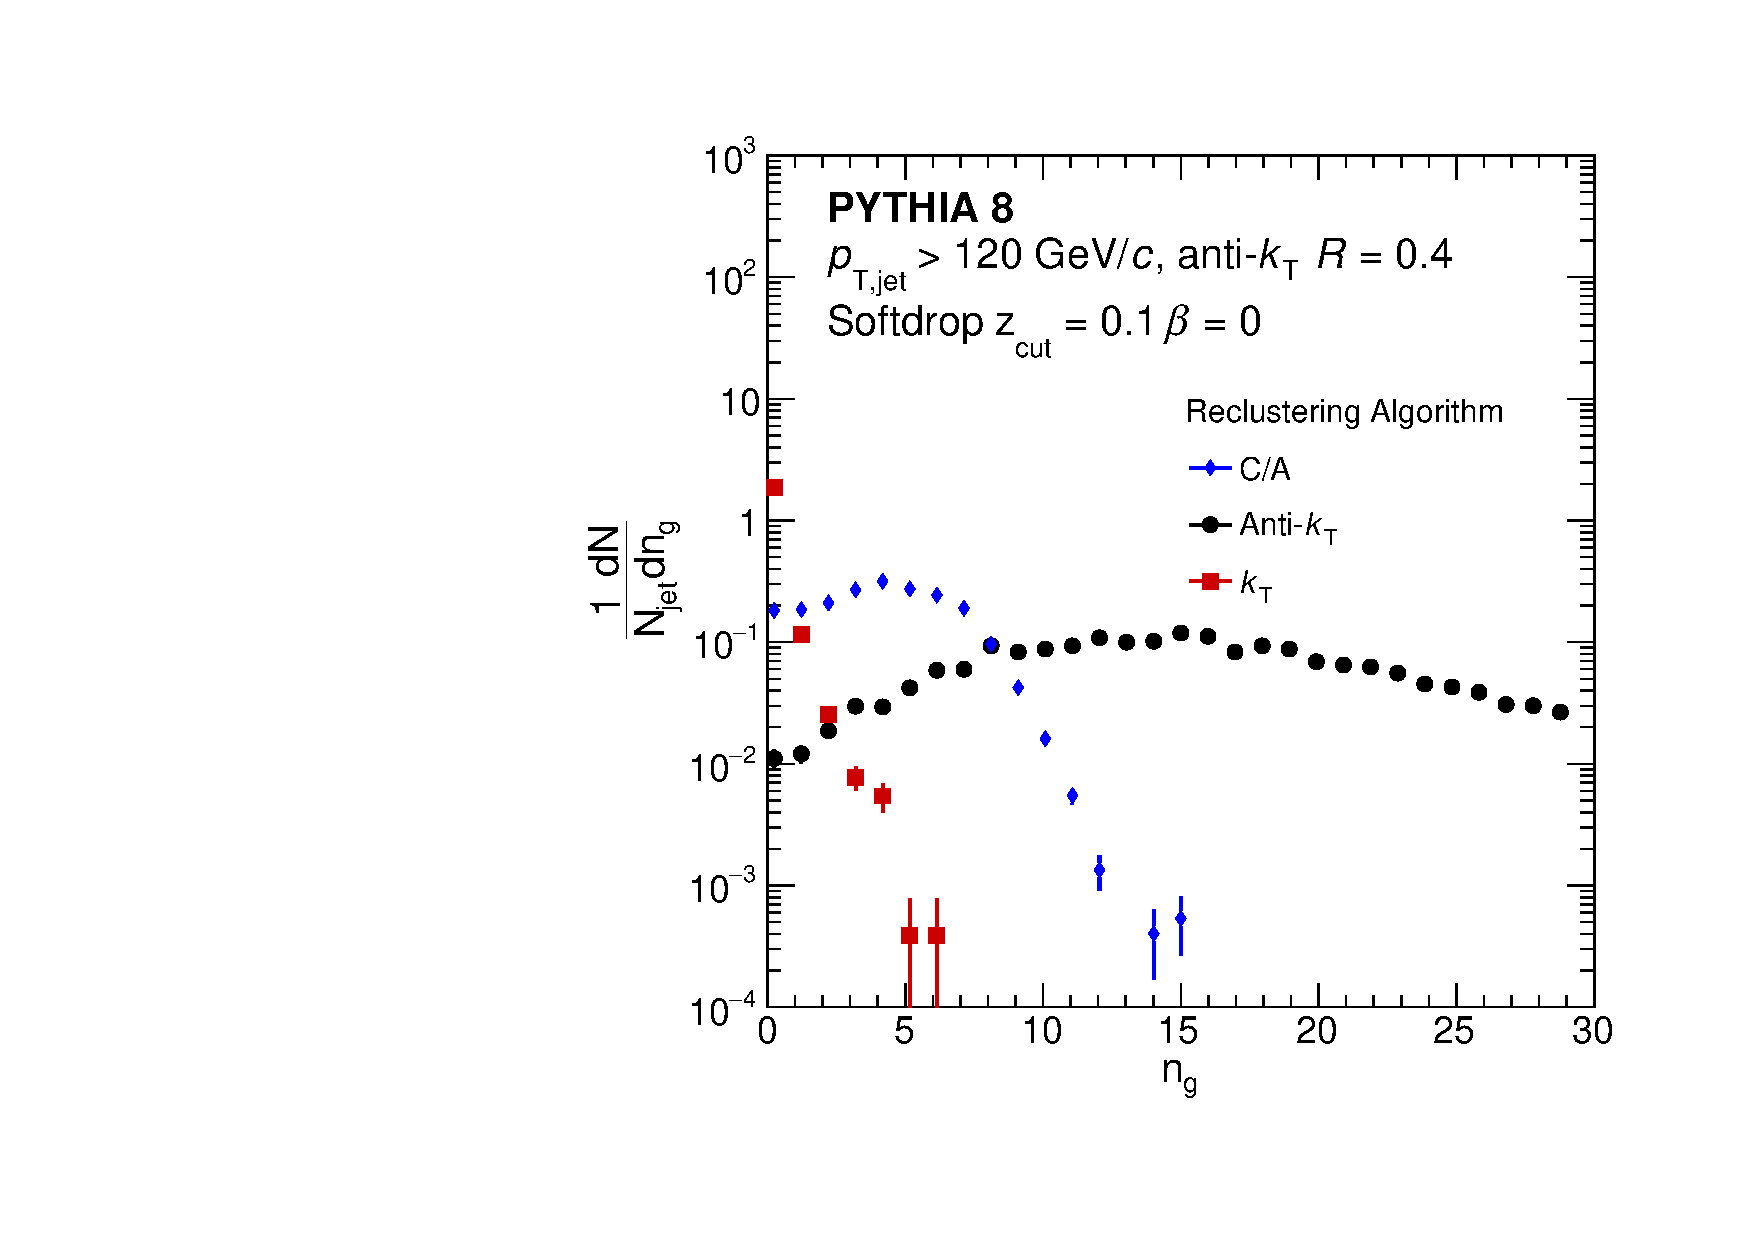
\includegraphics[width=0.4\textwidth]{figures/SDAlgorithms/ndropClusteringComp.pdf}%
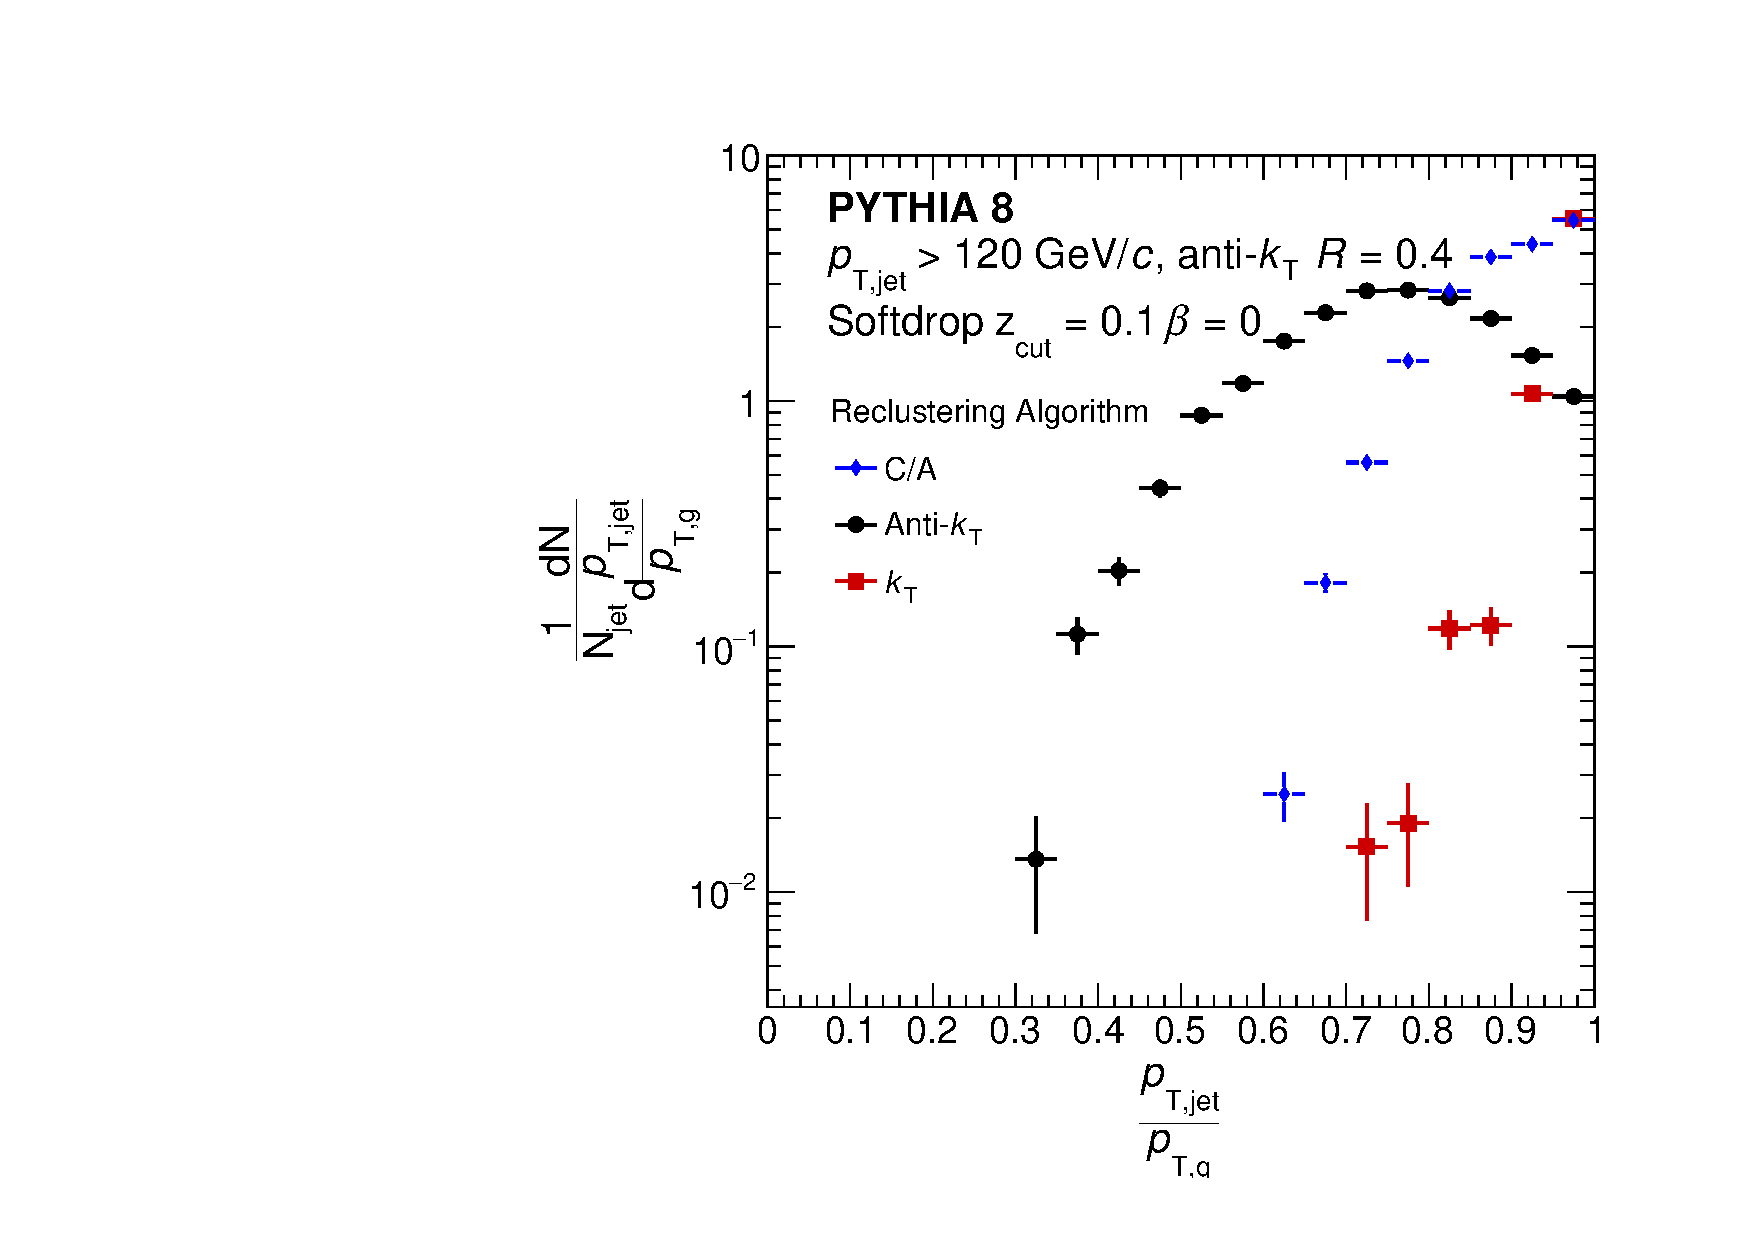
\includegraphics[width=0.4\textwidth]{figures/SDAlgorithms/ptratioClusteringComp.pdf}%
\caption{Effects of grooming on trees that are built up using different reclustering algorithms. Left plot: number of grooming steps. Right plot: ratio of jet $\pT$ before and after grooming.
}
\label{fig:PS2Vac_2}
\end{figure}
%%%%%%%%%%%%%%%%%%%%%%%%%%%%%%%%%%%%%
The change of algorithm also strongly affects what happens to the jet after grooming. In \autoref{fig:PS2Vac_2} (left), we show the distribution of the number of grooming steps for the three reconstruction algorithms discussed above. In particular, we note that the $k_\perp$ and the anti-$k_\perp$ algorithms result in completely different grooming. While the jet reconstructed with the former algorithm are mainly unaffected by grooming, in the latter case of the order of $\sim 10-20$ branches are groomed away. This also strongly affects the $\pT$ of the groomed jet, as seen in \autoref{fig:PS2Vac_2} (right), where the groomed jets in the anti-$\kT$ sample on average lose $\sim 20$\% of their energy. The C/A algorithm falls in between the two extremes, and is the only algorithm that maps the phase space with an approximately constant density, see \autoref{fig:PS2Vac} (left). Of the order of $\sim 5$ branches are removed by the grooming procedure on average, which slightly reduces the jet $\pT$ by $\lesssim 10$\%.

%%%%%%%%%%%%%%%%%%%%%%%%%%%%%%%%%%%%%
\begin{figure}[th]
\centering
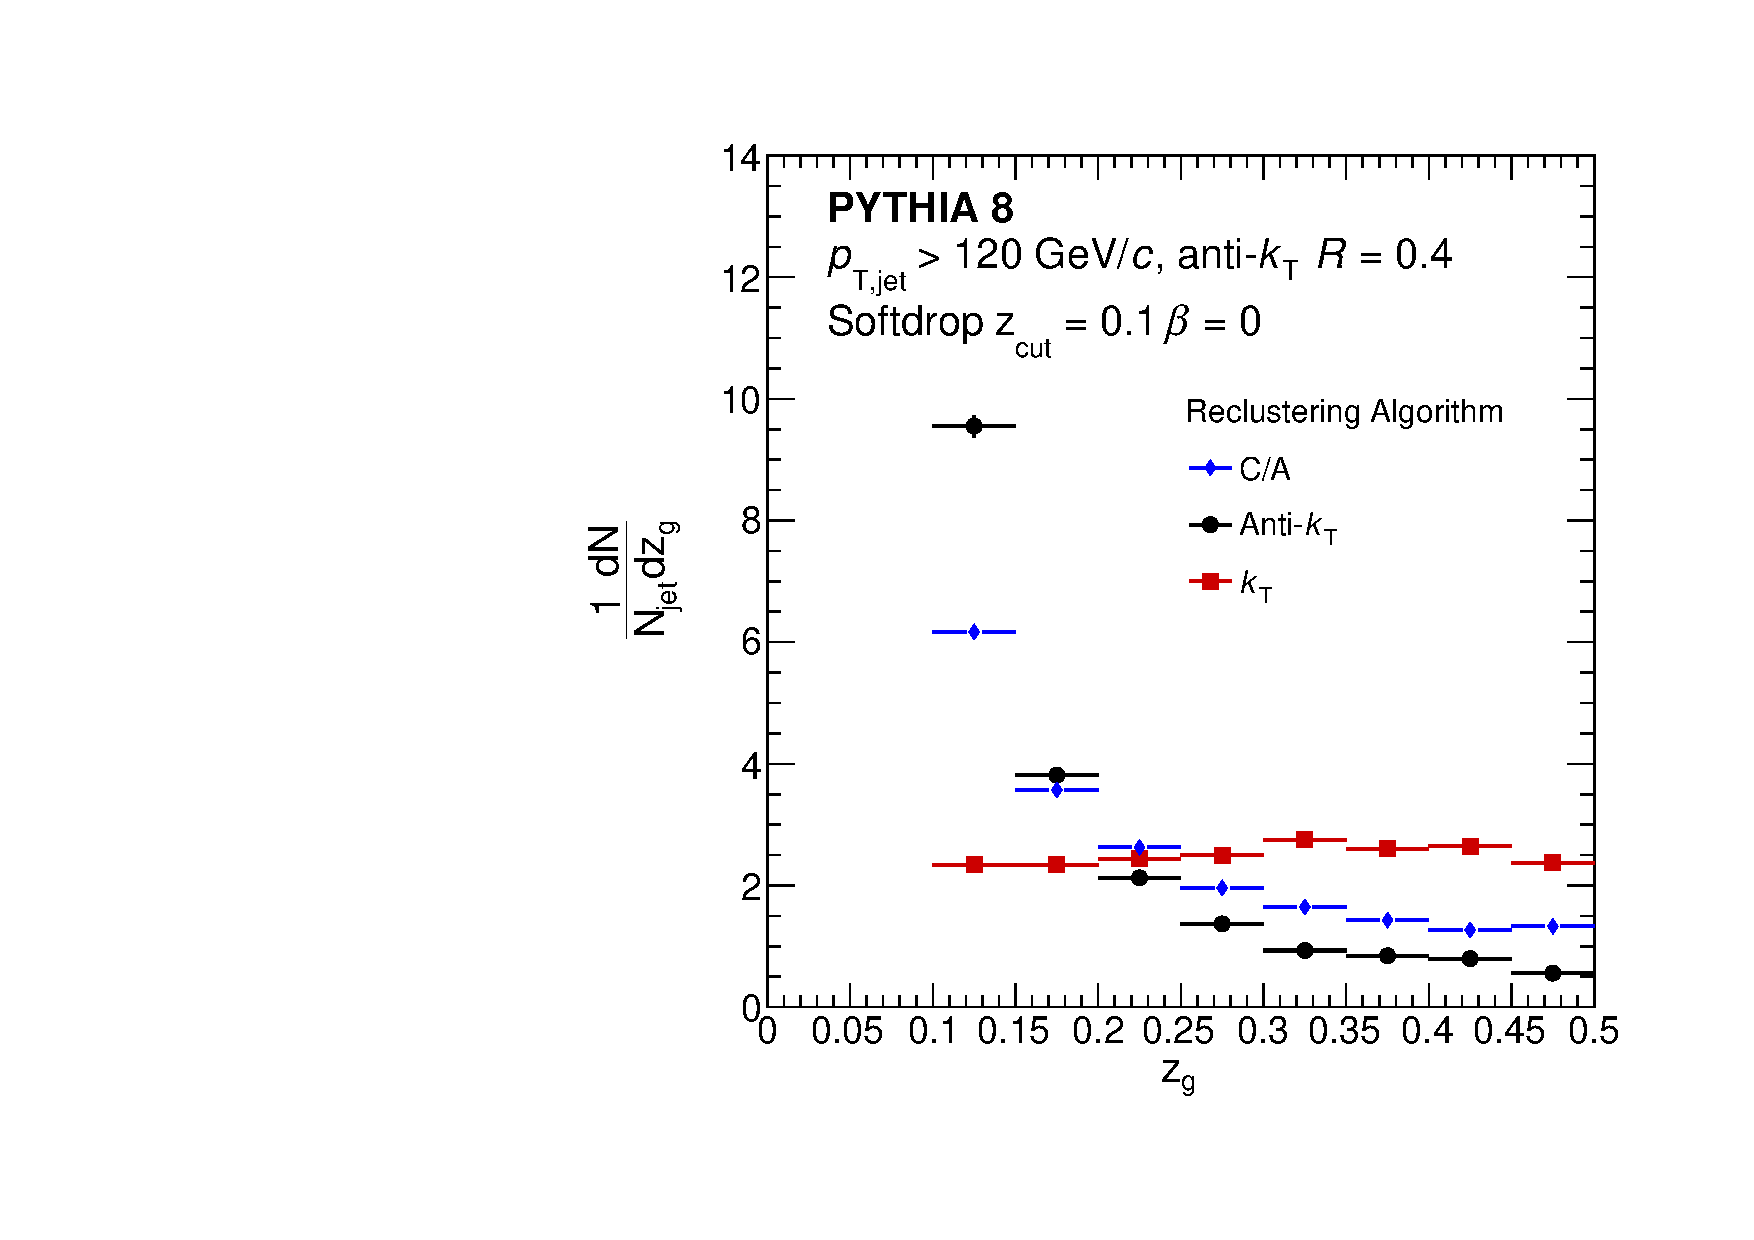
\includegraphics[width=0.32\textwidth]
{figures/SDAlgorithms/zgClusteringComp.pdf}
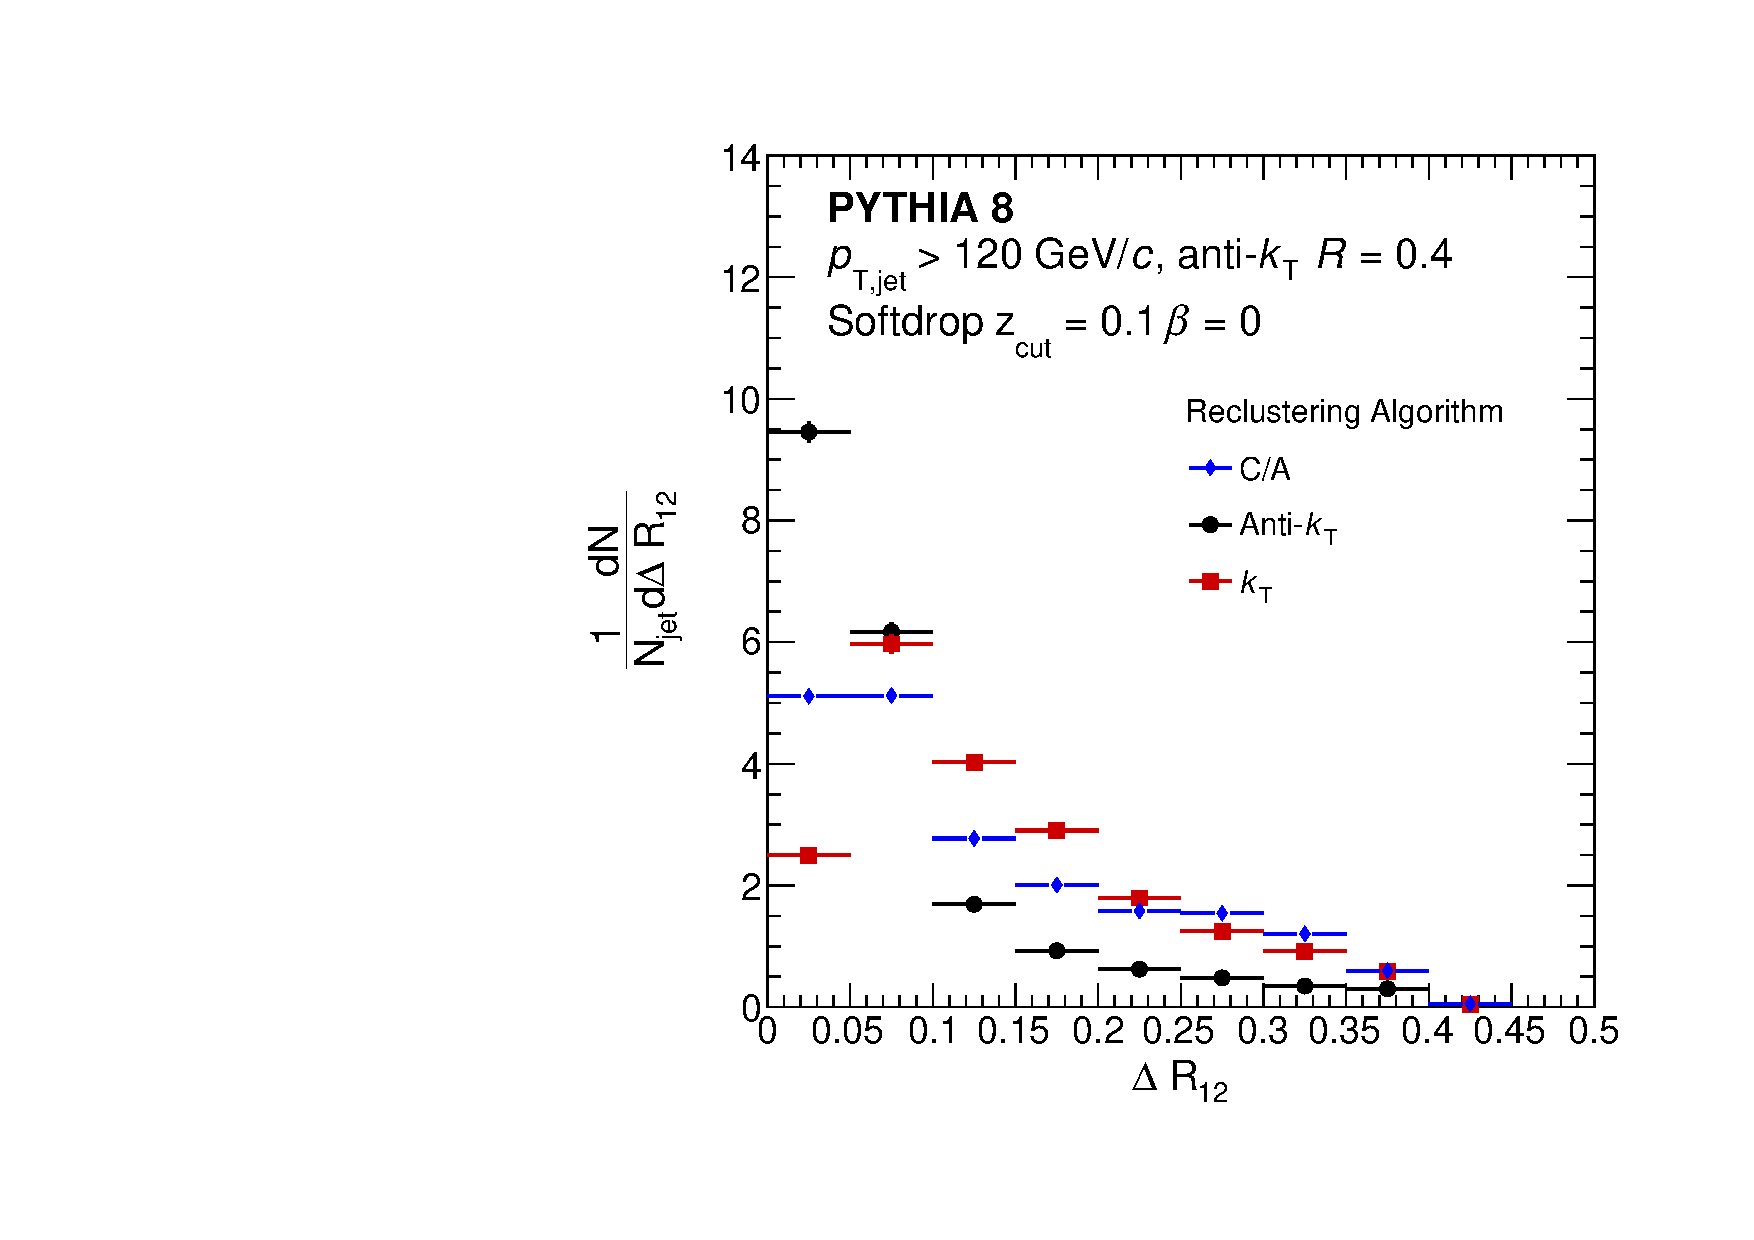
\includegraphics[width=0.32\textwidth]
{figures/SDAlgorithms/rgClusteringComp.pdf}
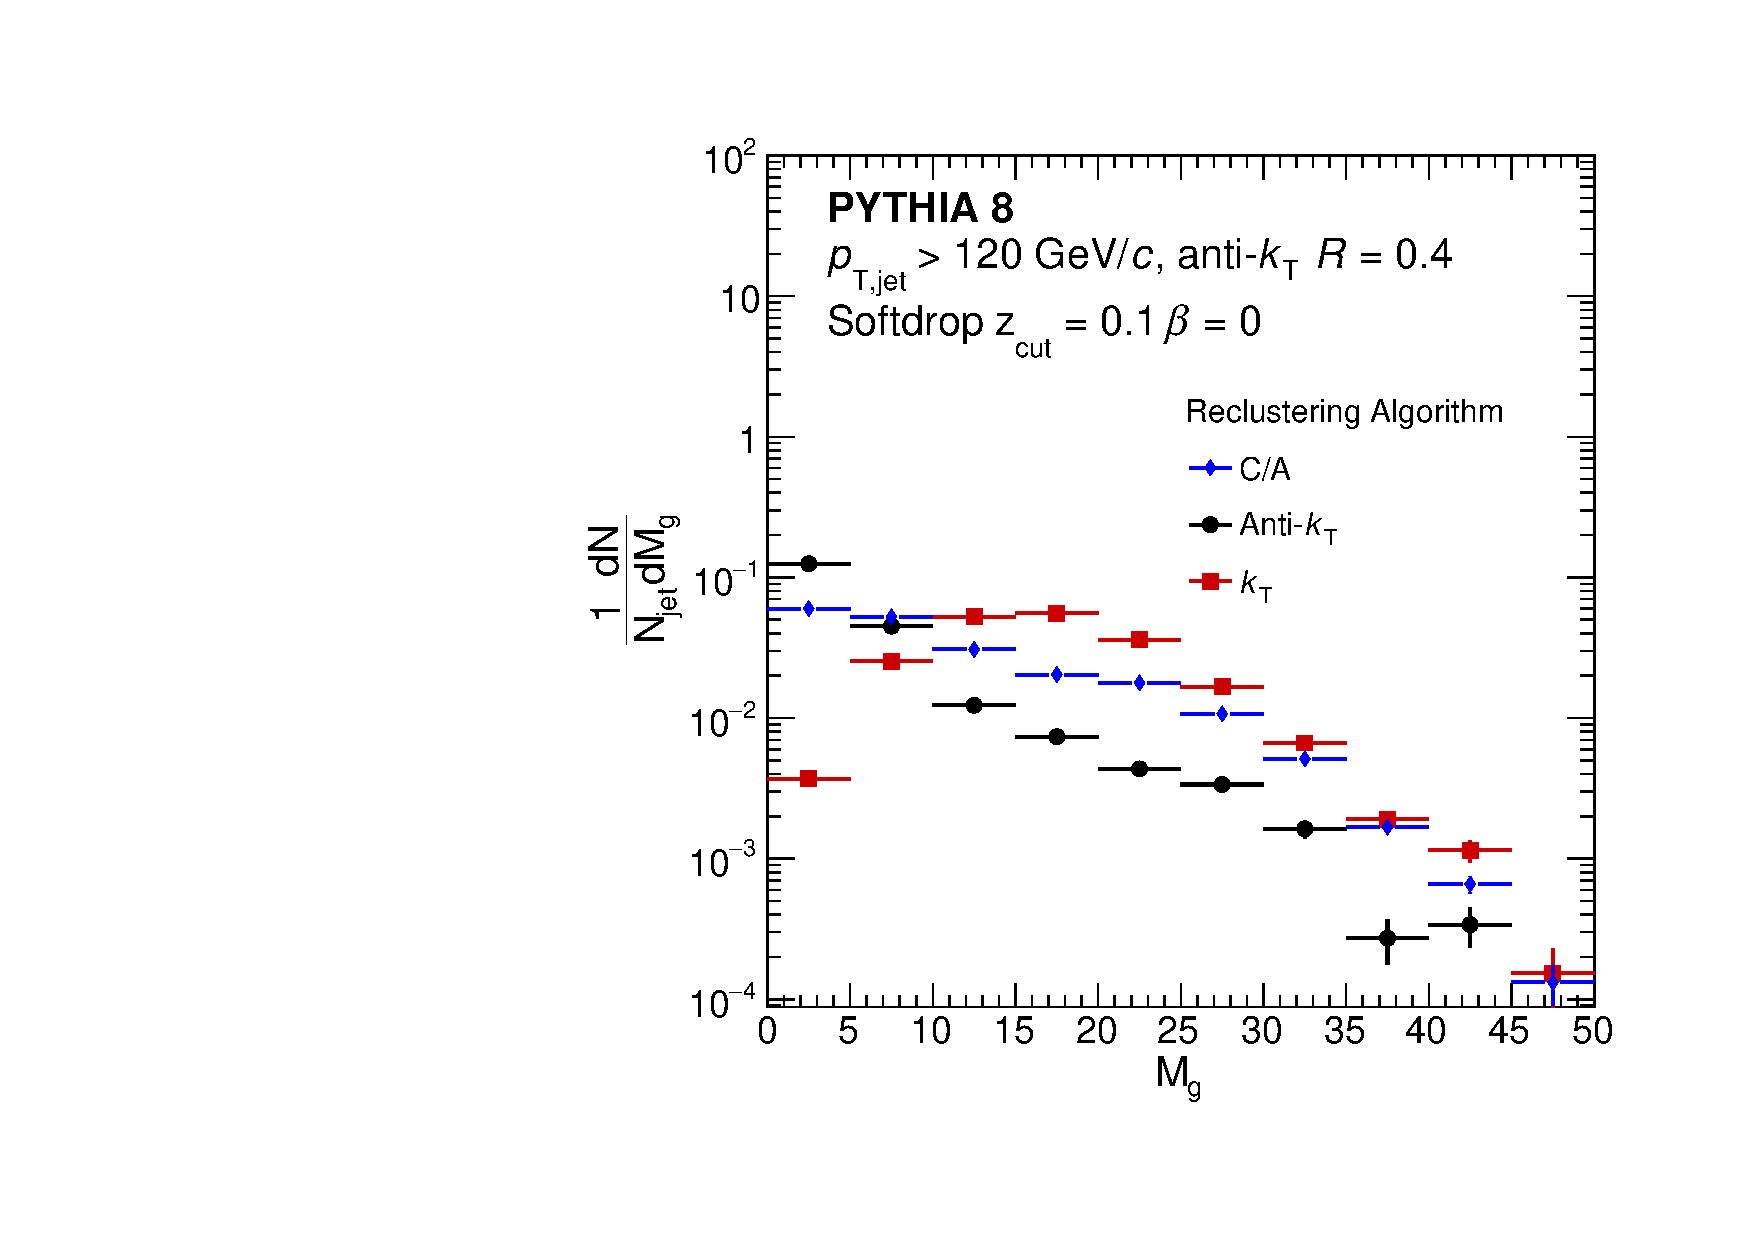
\includegraphics[width=0.32\textwidth]
{figures/SDAlgorithms/mgClusteringComp.pdf}%
\caption{Subset of grooming variables, symmetry parameter ($z_{g}$), groomed mass ($M_{g}$) and groomed radius ($\Delta R_{12}$) for three different jet reclustering algorithms.}
\label{fig:SDClusteringComp}
\end{figure}
%%%%%%%%%%%%%%%%%%%%%%%%%%%%%%%%%%%%%
Finally, we studied the behavior of the three observables subject to different reclustering algorithms applied, see \autoref{fig:SDClusteringComp}. In this particular case, we limit ourselves only to looking at the PYTHIA8 (vacuum) samples.
In case of a grooming prescription that requires a semi-hard splitting, for instance like in the SD1 setting,
%$z_{cut}$=0.1, $\beta=0$, 
the number of groomed branches will be large for anti-$k_{\rm \tiny T}$ reclustering ($\lesssim 30$) and very small for $k_{\rm \tiny T}$, for which the grooming conditions will be satisfied at the first iteration in most of the cases. Consistently, the groomed momentum fraction \zg\, probes very asymmetric splittings in the case of anti-$k_{\rm \tiny T}$ reclustering as can be seen in \autoref{fig:SDClusteringComp} (left). In contrast, $k_{\rm \tiny T}$-reclustered \zg\, picks exclusively up symmetric splittings, resulting in an almost featureless distribution. Similar conclusions can be made for the $\Delta R_{12}$ distribution, \autoref{fig:SDClusteringComp} (center), and $M_g$, \autoref{fig:SDClusteringComp} (right), as well. These artifacts are hard to reconcile with the expected behavior from QCD theory, and will therefore generally not be pursued further.


%%%%%%%%%%%%%%%%%%%%%%%%%%%%%%%%%%%%%%%%
\subsection{Enhancing jet quenching observables using grooming}
\label{sec:dissecting}
%%%%%%%%%%%%%%%%%%%%%%%%%%%%%%%%%%%%%%%%

Many jet quenching observables, such as the nuclear modification factor $R_{AA}$ and the momentum imbalance in photon-jet events, are considered benchmark measurements that quantify the amount of in-medium energy-loss and broadening. For reviews, see e.g. \cite{dEnterria:2009xfs,Majumder:2010qh}. However, their constraining power to discriminate between models have also been questioned. In some cases, the influence of background fluctuations can further obscure their constraining power.

In this section we present studies of conventional jet quenching observables that are enhanced by using grooming techniques.  As a first step, we apply SD grooming on the inclusive jet sample, extracting from each jet the grooming variables $z_g$ and $\Delta R_{12}$. 
This allows to further sub-divide the sample according to a measure involving these variables. 
For the purposes of this report, we have simply binned the fully inclusive sample according to the angle separating the two hardest subjets of a particular jet. This is motivated by the studies using splitting maps and the results obtained for the substructure observables previously. Another motivation is to differentiate between the modifications of the ``soft'' and the ``hard'' structure of the jet. The former is more dominant for inclusive observables and for non-restrictive SD settings, e.g. SD1 and SD2 in \autoref{fig:TheorySD} (left and central panels), while the latter would be more pronounced for conservative SD parameter choices, such as SD3 in \autoref{fig:TheorySD} (right panel).

Due to the limited scope of the workshop, we have not attempted to study this in any systematic way. Here, we only report on the two following studies at LHC energies:
\begin{itemize} 

\item the nuclear modification factor $R_{AA}$ binned in the angular separation $\Delta R_{12}$ as found with SD2.

\item the $x_{J\gamma}$ distribution binned in the angular separation $\Delta R_{12}$ as found with SD1. 
\end{itemize}
For both grooming settings, comparing small- and large-angle substructure configurations also gives an additional handle on the formation time of that particular splitting, see \autoref{fig:PS0} (right).

In both cases, jets were reclustered and groomed, and only jets that had a candidate subjet pair that fulfilled the Soft Drop condition were further analyzed.
More importantly, all results in this section have been computed by embedding the MC jet samples into a realistic, centrality-dependent heavy-ion background, for details see \kmt{where?}. Therefore, these result reflect more realistically the magnitude of effects that should be expected to arise in heavy-ion collisions at the LHC.
%{\color{red} Are the curves for $\Delta R>0.3$ consistent with the expected effect of uncorrelated background at large angles...? Was additional pile-up mitigation employed?}

The well-known nuclear modification factor $R_{AA}$ compares the yields of equivalent hard processes in heavy-ions and proton-proton collisions, and is given schematically as
\beq
\label{eq:RAA}
R_{AA} = \frac{\dd N_{AA}/\dd \pT^2 \dd y}{\langle N_\text{coll} \rangle \dd N_{pp}/\dd \pT^2 \dd y} \,,
\eeq
where $\langle N_\text{coll} \rangle$ counts the number of nucleon-nucleon collisions in a given centrality range,
is a standard benchmark for estimating/tuning medium parameters in theoretical calculations and Monte Carlo jet quenching models. By dividing the sample of inclusive high-$\pT$ jets into small- and large-angle configurations, we obtain more differential information regarding the accompanying modifications of the intra-jet structure. Similar studies, albeit using another method to dissect the jet sample into two-prong structures, was already presented in \cite{Zhang:2015trf,Apolinario:2017qay}.
Note, however, that the suggested ``binning'' procedure could be sensitive to different physical mechanisms separately in the proton-proton and heavy-ion events. Disentangling this would demand further studies.

%%%%%%%%%%%%%%%%%%%%%%%%%%%%%%%%%%%%%
\begin{figure}[th]
\centering
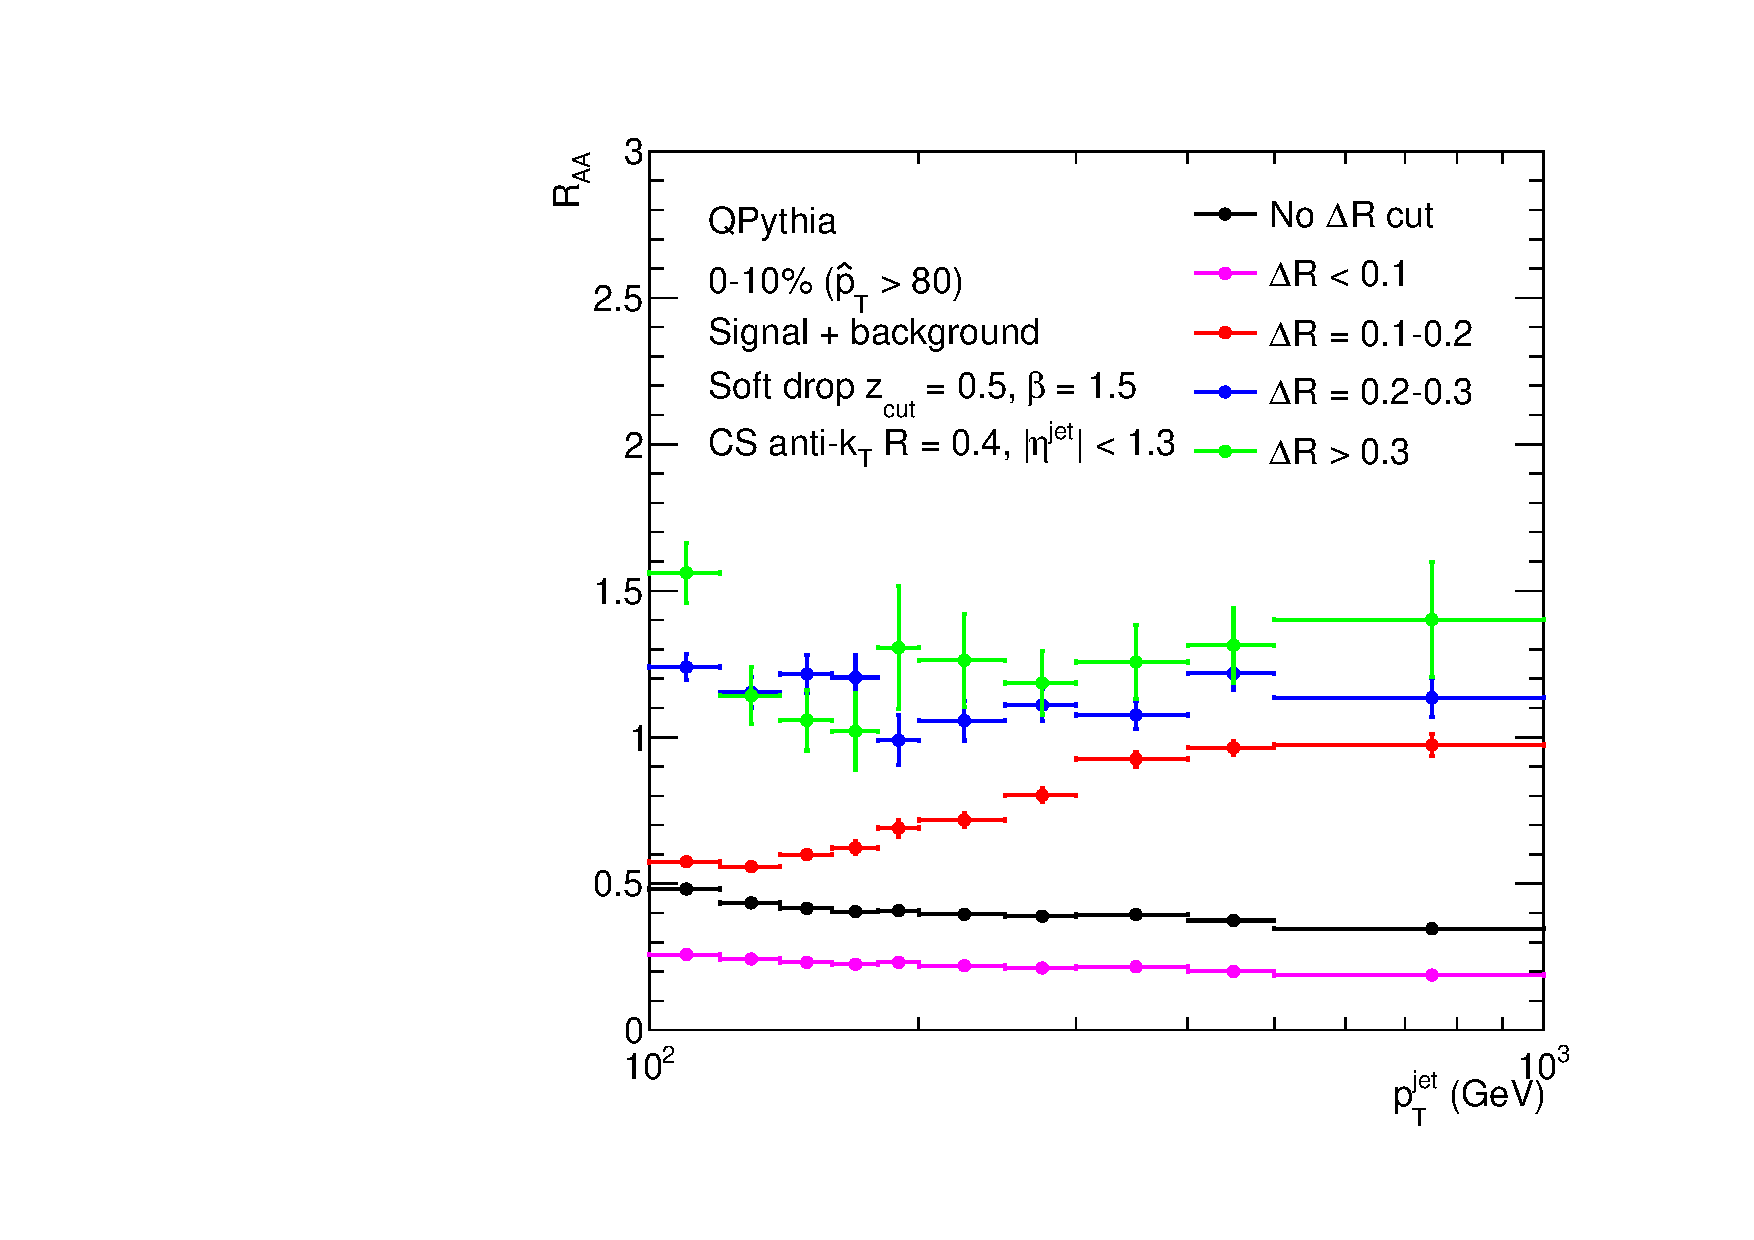
\includegraphics[width=0.32\textwidth]{figures/Observables_RAA/Plot9}
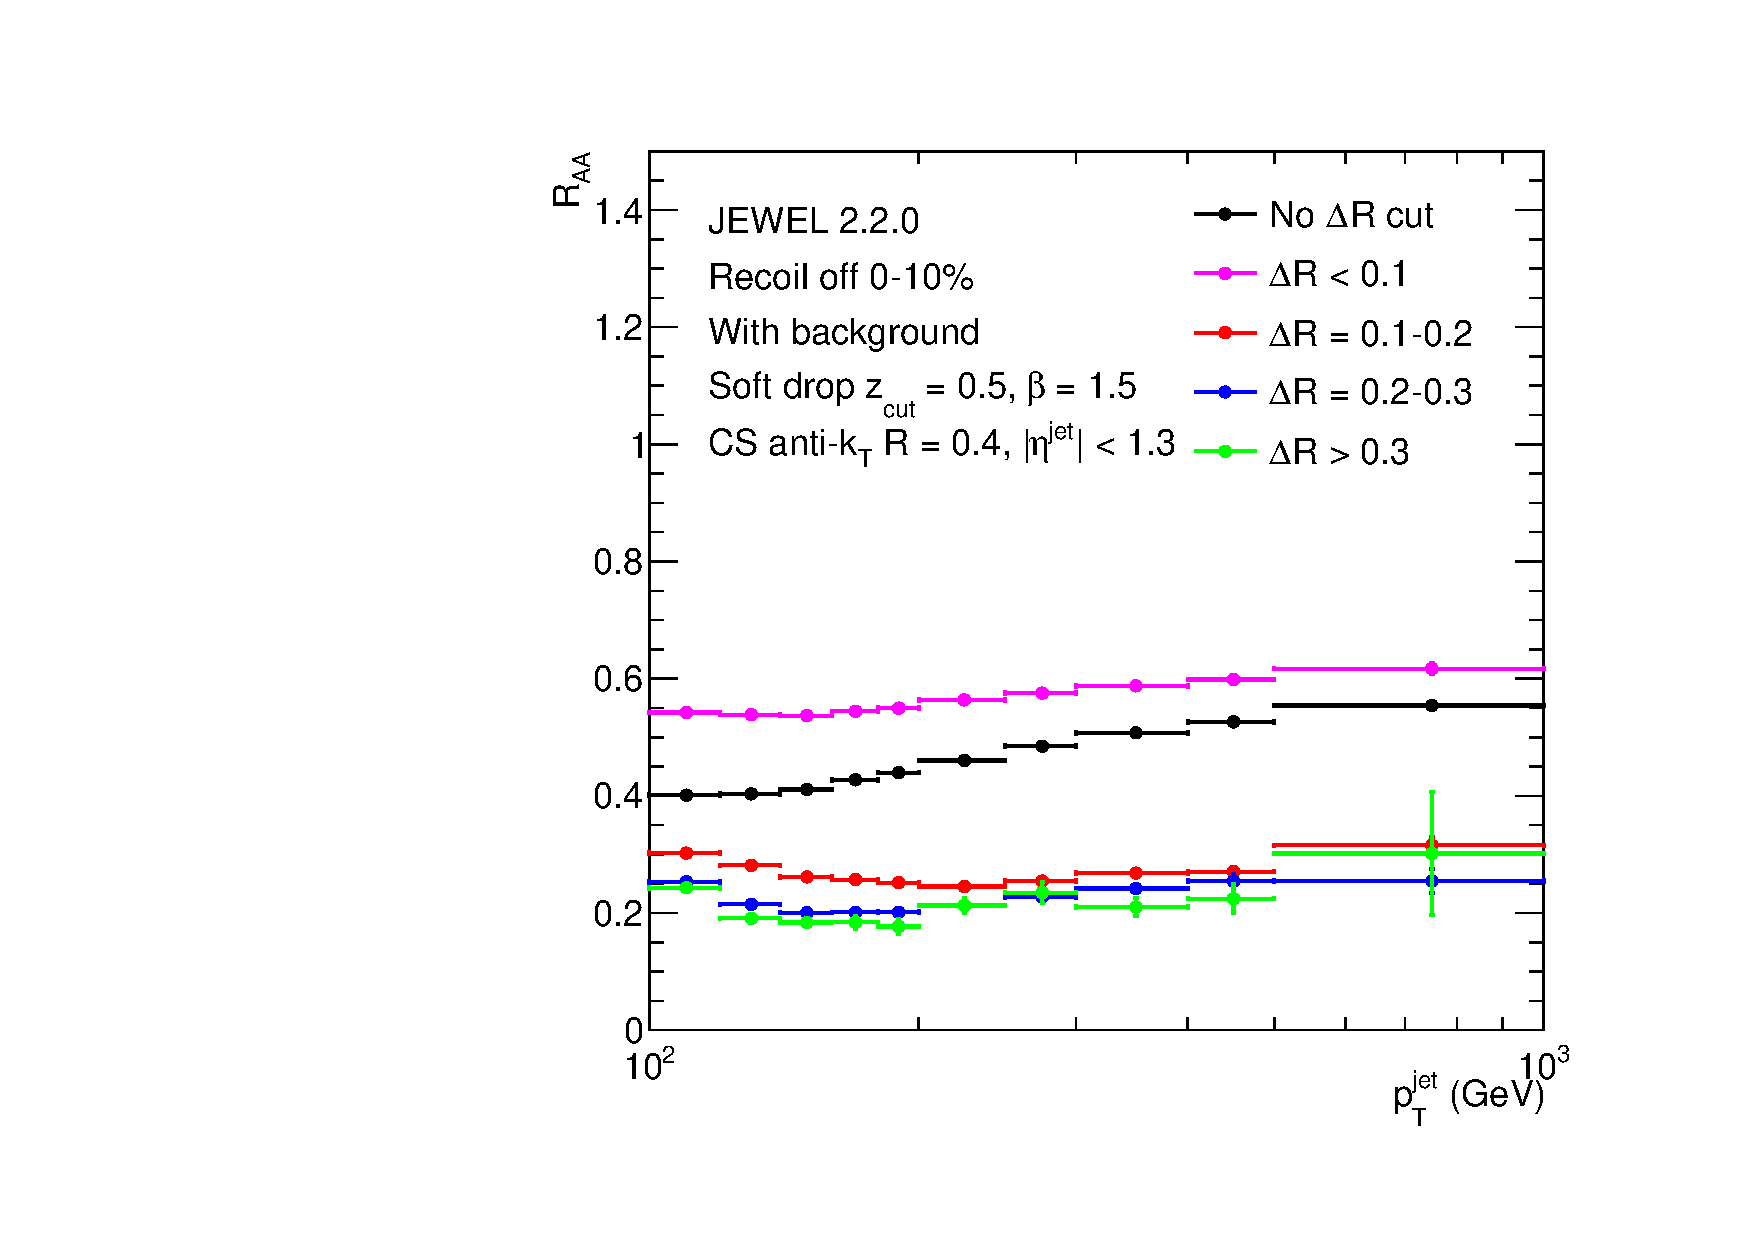
\includegraphics[width=0.32\textwidth]{figures/Observables_RAA/Plot3}
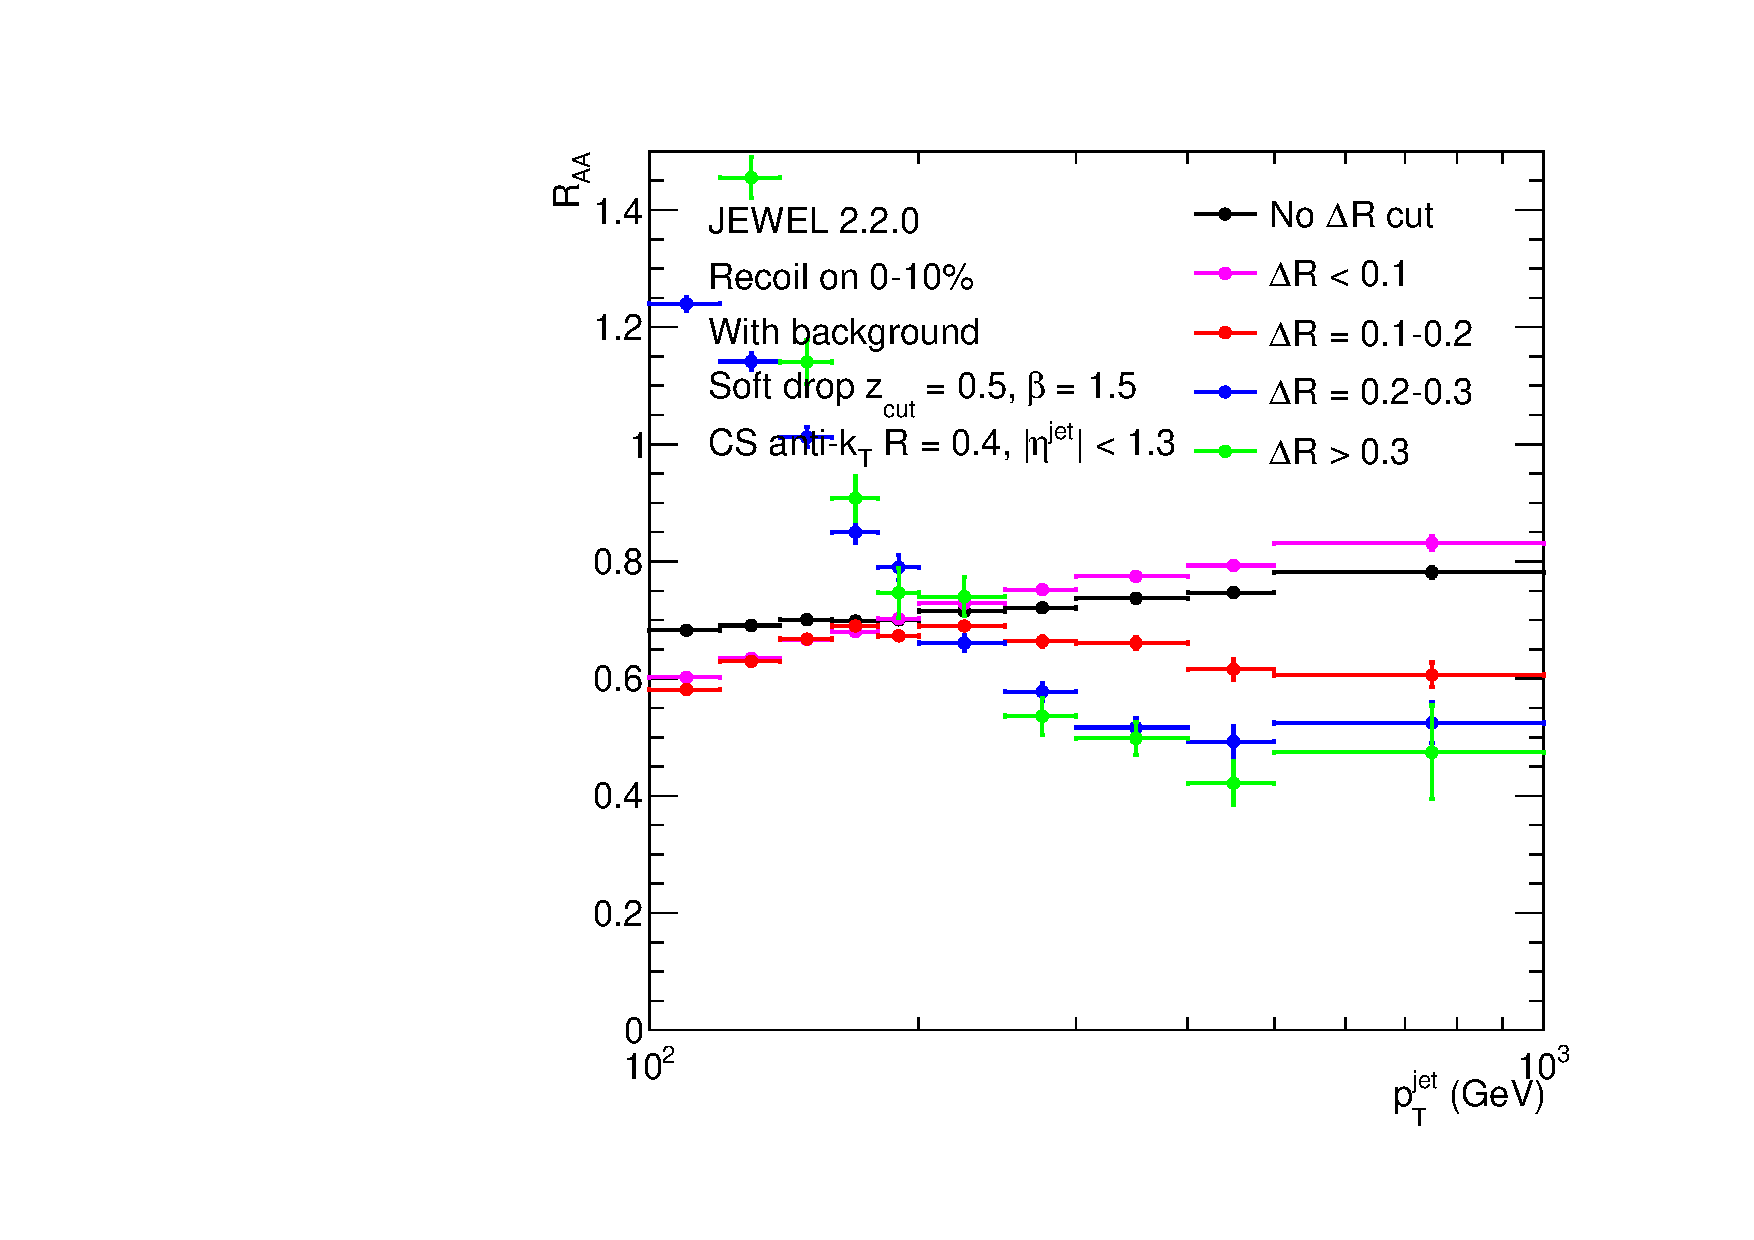
\includegraphics[width=0.32\textwidth]{figures/Observables_RAA/Plot4}
%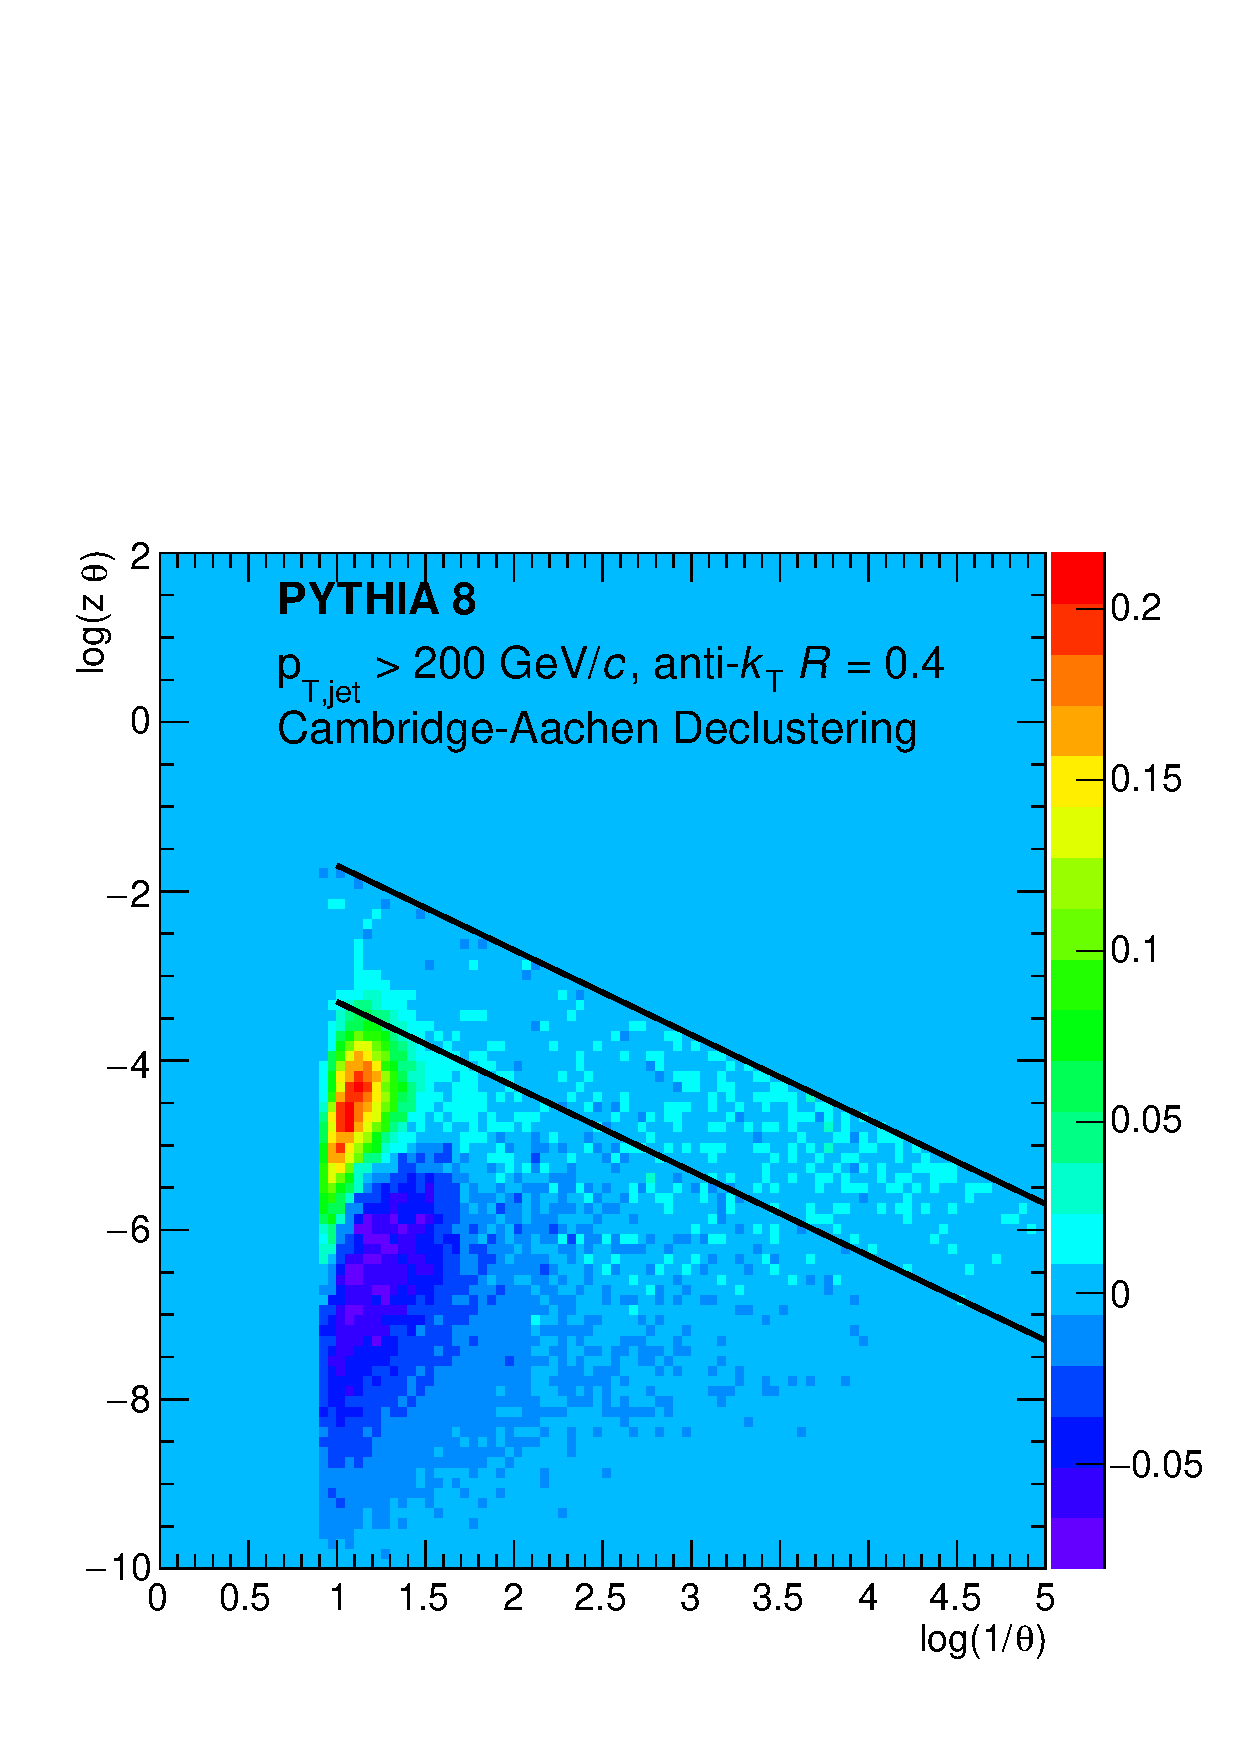
\includegraphics[width=0.33\textwidth]{figures/LundMC/PythiaDiffCA_wLines200.pdf}%
%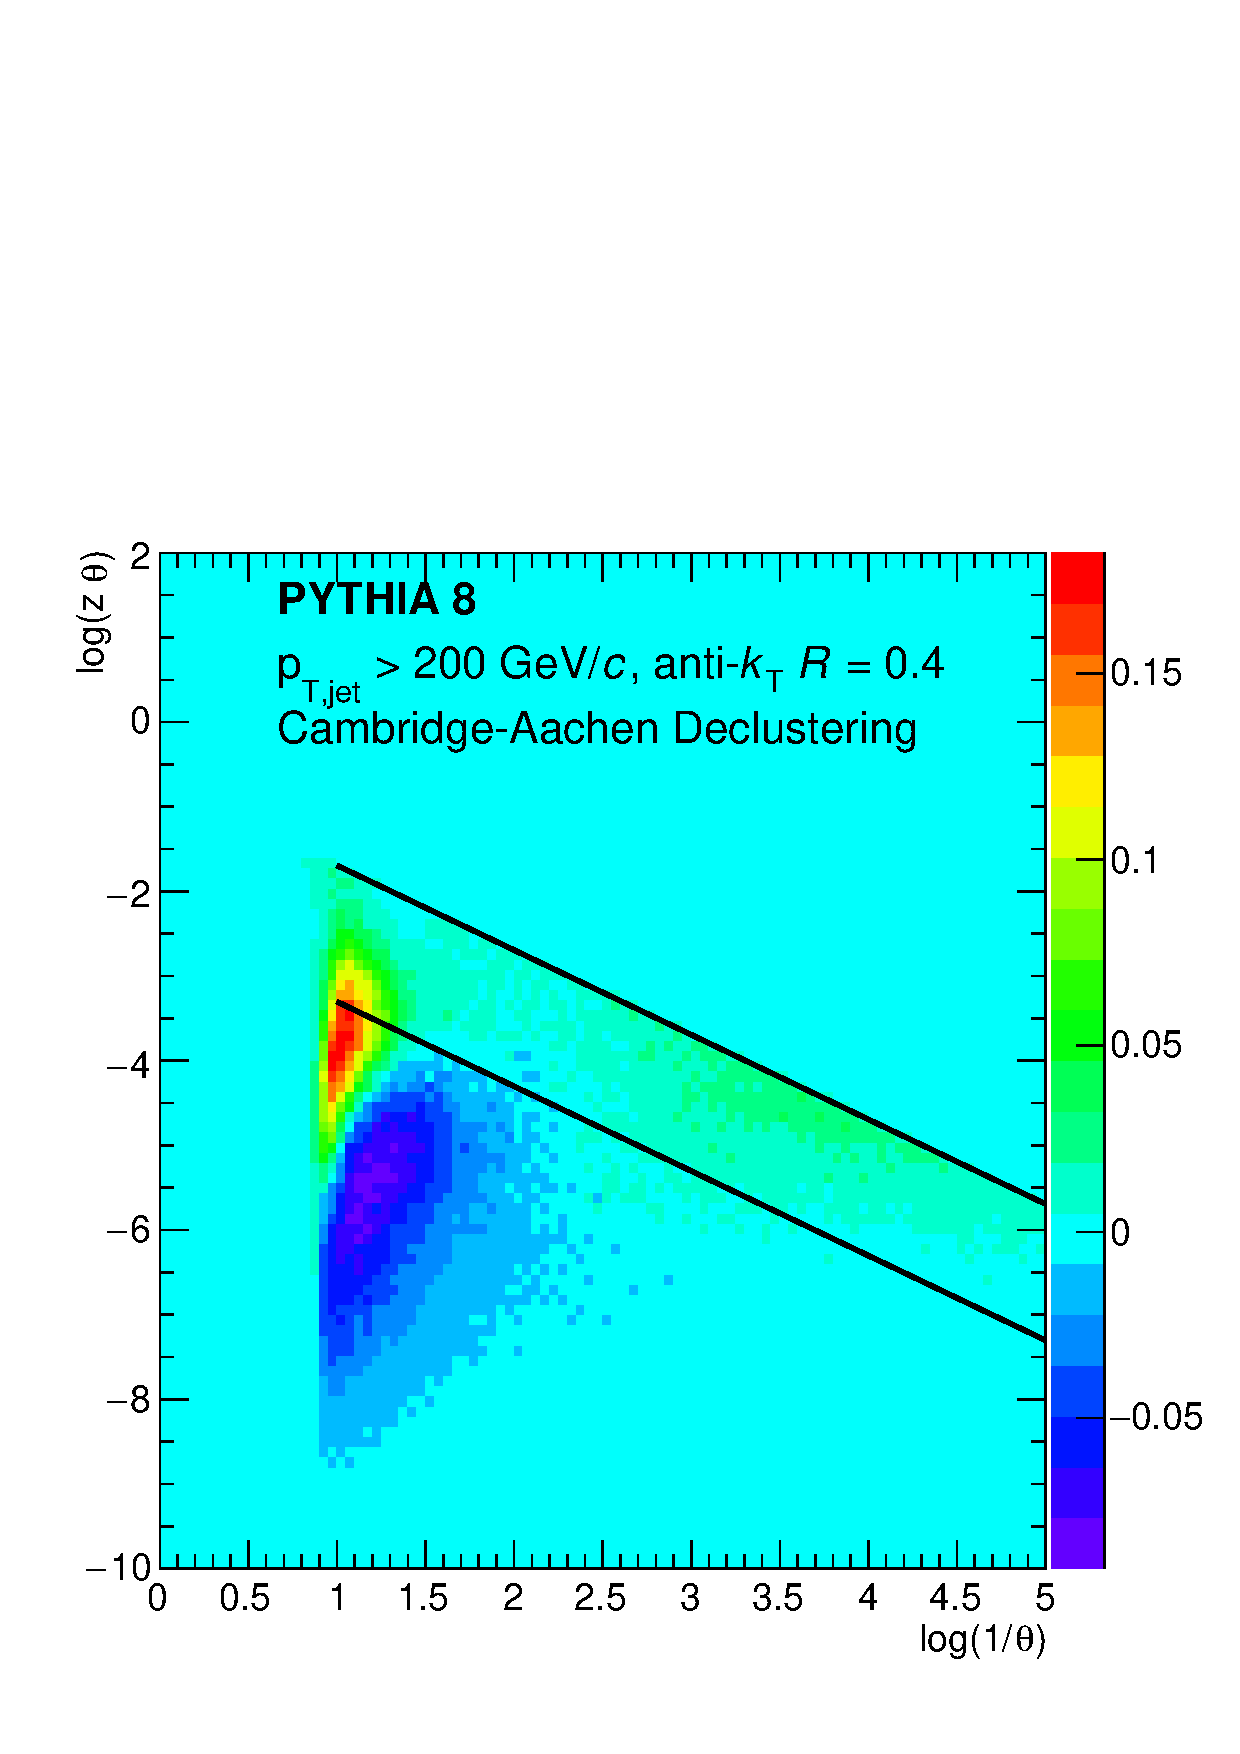
\includegraphics[width=0.33\textwidth]{figures/LundMC/PythiaDiffCA_wLines80120.pdf}%
\caption{The nuclear modification factor for subsamples of jets that have been unrolled as a function of $\Delta R$ of the leading sub-jets identified using SD1. 
}
\label{fig:GroomedRAA}
\end{figure}
%%%%%%%%%%%%%%%%%%%%%%%%%%%%%%%%%%%%%
The jet samples generated from QPYTHIA, JEWEL ``Recoil off'' and JEWEL ``Recoil on'' that goes into calculating $R_{AA}$ in \autoref{fig:GroomedRAA}, has been binned according to the angular separation of the subjets identified using SD3 grooming, $\Delta R_{12}$. While all three models show a similar transverse momentum dependence of $R_{AA}$ for the fully inclusive sample (see black points in \autoref{fig:GroomedRAA}), large differences are seen for the more differential  results.\footnote{The overall magnitude of the inclusive $R_{AA}$ does not play an important role for the point we are trying to make here.} 

In QPYTHIA, the core of the jet is quenched stronger than the periphery, as expected from previous studies above, see \autoref{fig:GroomedRAA} (left). It is basically related to the enhanced splitting of collinear modes. For the JEWEL ``Recoils off'' sample, see \autoref{fig:GroomedRAA} (center), the effect is completely opposite: the jet core is quenched much less than large-angle configurations. This also comes as no surprise in light  of other substructure observables that were analyzed above, see e.g. \autoref{sec:groomedobservables}, and reflects stronger energy-loss effects for large-angle substructure fluctuations which implies that more partons are quenched \cite{Milhano:2015mng}. Finally including recoil effects, the JEWEL ``Recoils on'' sample, see \autoref{fig:GroomedRAA} (right), reveal a strong $\pT$-dependence of large-angle jets, leading to a big enhancement of $R_{AA}$ at relatively low transverse momenta. This implies of an enhanced constraining power to details of medium recoil modeling in this observable.

Other benchmark observable in heavy-ion collisions include the $Z$-jet or photon-jet momentum asymmetry. Here, we will only focus on the latter.
We recall that the variable $x_{J\gamma}$ is defined as the ratio of jet to photon momentum, 
\beq
x_{J\gamma} = \frac{p_\text{{\tiny T},jet}}{p_{\text{\tiny T},\gamma}} \,.
\eeq
In contrast to the nuclear modification factor \eqref{eq:RAA}, this observable does not immediately involve a comparison to a proton-proton baseline. The direct access to the photon energy in the measurement also would help constrain the effect of energy-loss or migration of jets between $\pT$-bins.

%%%%%%%%%%%%%%%%%%%%%%%%%%%%%%%%%%%%%
\begin{figure}[th]
\centering
%\includegraphics[width=0.5\textwidth]
%{figures/Observables_GammaJet/GammaJet_groomed}%
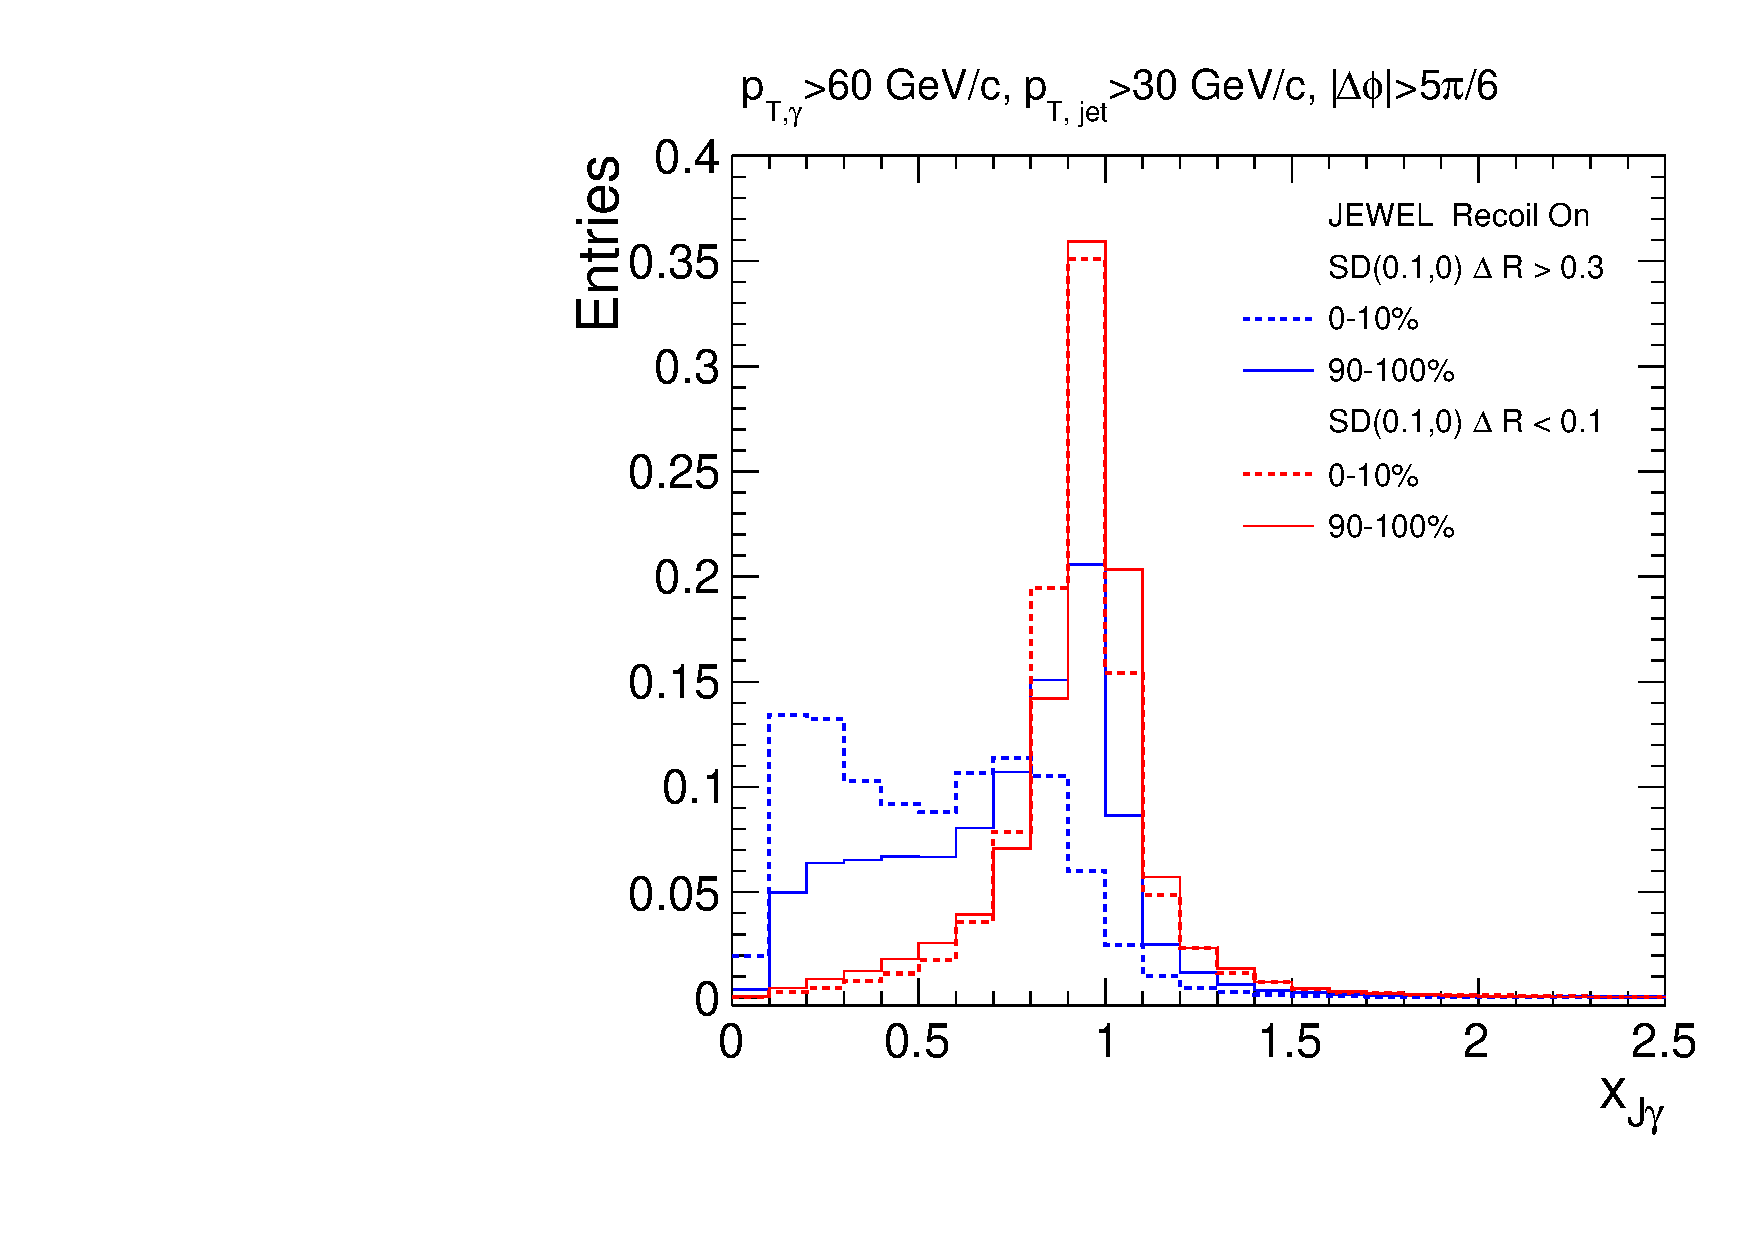
\includegraphics[width=0.5\textwidth]
{figures/Observables_GammaJet/JEWEL-photon-jet-recoilOn-linear}%
\caption{The $x_{J\gamma}$ distribution for subsamples of jets that have been unrolled as a function of the angle found between the leading sub-jets using SD. }
\label{fig:GroomedGammaJet}
\end{figure}
%%%%%%%%%%%%%%%%%%%%%%%%%%%%%%%%%%%%%
In \autoref{fig:GroomedGammaJet} we present the resulting $x_{J\gamma}$ distribution for the JEWEL ``Recoils on'' samples in two centrality bins (corresponding to $0-10$\% and $90-100$\% centrality). This sample has been binned in subjet angular separation, as described above, this time using SD2 grooming. The same features that have been pointed out multiple times, also show up here as a function of collision centrality. Notably, the small-angle sample shows very little dependence of centrality, and is closely peaked around 1. The large-angle sample, on the other hand, which also corresponds to jets formed earlier in the medium, is strongly distorted. While the distribution for  90-100\% centrality is broader for the large-angle sample, we observe that the peak structure, which is clearly visible in \autoref{fig:GroomedGammaJet}), is completely removed when going to the most central collisions. 
%\kmt{Features: groomed substructure gives us access to binning in formation time of that splitting of substructures; large angle sample is strongly modified! Very constraining for recoil modeling..? No need for pp baseline (often binning in ``heavy-ion-modified'' variables sample completely different processes in pp and AA. }
\kmt{Can we get a result for QPYTHIA?}

These proof-of-principle studies illustrate the enhanced sensitivity to more than one variable that can be obtained by differentiating the inclusive jet sample using a well-controlled procedures. 
In this section, we have analyzed medium-modified jet samples embedded in a heavy-ion background and utilized the angular separation between the leading subjets, as extracted Soft Drop procedure, in order to bin the jets into small- and large-angle configurations. While this should not come as a surprise in light of the previous results on the groomed substructure observables $z_g$, $\Delta R_{12}$ and $M_g/\pT$, we observe very different modification patters between the employed models and potentially large effects. Measurements of jets recoiling from $Z$-bosons or photons could prove as especially valuable in tracking how jets are modified in all variables, including the overall $\pT$ shift.
However, the results presented in this section are only exploratory and more systematic studies are left for the future.
